\documentclass[12pt]{report}

\usepackage{setspace}
\renewcommand{\baselinestretch}{1.5}
\usepackage{float}
\usepackage{lipsum}
\usepackage{multirow}
\usepackage{graphicx}
\usepackage{subcaption}
\usepackage[table,xcdraw,dvipsnames]{xcolor}
\usepackage{lscape}
\usepackage{titlesec}
\usepackage{titletoc}
\usepackage{titling}
\usepackage[T1]{fontenc}
\usepackage[utf8x]{inputenc}
\usepackage{amsmath}
\usepackage{caption}
\usepackage{adjustbox}
%\usepackage[a4paper,margin=0.5in]{geometry}
\usepackage[a4paper,%
            left=2cm,right=2cm,top=1cm,bottom=2cm,%
            footskip=-1cm]{geometry}
\usepackage[normalem]{ulem}
\usepackage[none]{hyphenat}
\usepackage[hidelinks]{hyperref}
\PassOptionsToPackage{hyphens}{url}\usepackage{hyperref}
\useunder{\uline}{\ul}{}

% No hyphenation (word wrapping) with text justification
\tolerance=1
\emergencystretch=\maxdimen
\hyphenpenalty=10000
\hbadness=10000

% Replace table caption name
\usepackage{caption}
% \captionsetup[table]{name=Table}

% For toc, lot and lof
\usepackage[titles]{tocloft}

% For liste of figures and tables!
\graphicspath{{./images/}}
\usepackage{array}

% Font options
\usepackage{mathptmx}
%\usepackage{tgtermes}
%\usepackage{tgpagella}
%\usepackage{helvet}
%\usepackage{tgbonum}

% fancy logo for page numbers!
\usepackage{fancyhdr,blindtext,tikz}
\usepackage{lastpage,refcount}

% Box frame for figures #\fbox{}
\setlength{\fboxsep}{0pt}
\setlength{\fboxrule}{0.69pt}

% Options: Sonny, Lenny, Glenn, Conny, Rejne, Bjarne, Bjornstrup
\usepackage[Conny]{fncychap}

%package for inserting raw text files
\usepackage{verbatim}
\usepackage{listings}

% Redifining from 0.1 to 1 ... 2 ... and so on
\renewcommand{\thesection}{\arabic{section}}

% Renaming Bibliography name
\renewcommand\bibname{References}

% Bibliography styling
\bibliographystyle{plain}

% Redifining from 1.1 to 1.a ... 1.b ... and so on
%\renewcommand{\thesubsection}{\alph{subsection}}

% Part rules
\titlecontents{part}[1em]
{\vskip 0.5ex}%
{}% numbered sections formatting
{\itshape\scshape}% unnumbered sections formatting
{}%

% Chapter rules
\titlecontents{chapter}[1em]
{\vskip 0.5ex}%
{}% numbered sections formatting
{\itshape\scshape}% unnumbered sections formatting
{\titlerule*[0.3pc]{.}\contentspage}%

% Section rules
\titlecontents{section}[1em]
{\vskip 0.2ex}%
{\hspace{0.15in}\contentslabel{0.13in}.\hspace{0.1in}}% numbered sections formatting
{\itshape}% unnumbered sections formatting
{\titlerule*[0.3pc]{.}\contentspage}%

% Subsection rules
\titlecontents{subsection}[3.5em]
{}%
{\contentslabel{0.10in}\hspace{0.25in}}% numbered sections formatting
{}% unnumbered sections formatting
{\titlerule*[0.3pc]{.}\contentspage}%

% Custom colors!
\definecolor{MYCOL}{HTML}{00318A}

% List of Figures settings:
\renewcommand{\listfigurename}{Liste Of Figures}
\renewcommand{\cftloftitlefont}{\vspace*{-0.6in}\hfill\color{Black}\fontsize{35}{43}\bfseries}
\renewcommand{\cftafterloftitle}{\hfill}
\setlength{\cftfigindent}{0pt} % left aligned Fig entries
\renewcommand{\cftfigpresnum}{Figure } % put before the number
\renewcommand{\cftfigaftersnum}{:} % put before the number
\addtolength{\cftfignumwidth}{2.5em} % extra space for \cftpresnum

% List of Tables settings:
\renewcommand{\listtablename}{Liste Of Tables}
\renewcommand{\cftlottitlefont}{\vspace*{-0.6in}\hfill\color{Black}\fontsize{35}{43}\bfseries}
\renewcommand{\cftafterlottitle}{\hfill}
\setlength{\cfttabindent}{0pt} % left aligned Tab entries
\renewcommand{\cfttabpresnum}{Table } % put before the number
\renewcommand{\cfttabaftersnum}{:} % put before the number
\addtolength{\cfttabnumwidth}{2.5em} % extra space for \cftpresnum

% Table of contents settings:
\renewcommand{\contentsname}{Table Des Matières}

\usepackage[framemethod=TikZ]{mdframed}

% My custom page style
\fancypagestyle{myfancy}{%   
   \fancyhf{}%
   \fancyfoot[C]{\tikz[baseline={(0,0)},anchor=center] \node[label={center:\thepage}]{\includegraphics[scale=.037]{../images/cloud.png}};}%
   \renewcommand{\headrulewidth}{0pt}%
   \renewcommand{\footrulewidth}{0pt}%
   \fancyhead{}
   \fancyfoot{}
   \fancyfoot[C]{\vspace{-0.42in}\textcolor{Gray}{\Large{Page}}\hspace{0.04in} \large{\thepage}\hspace{0.07in}\large{|}\hspace{0.07in}\large{\pageref{LastPage}}}
}%
\pagestyle{empty}

% Custom environment
\newenvironment{changemargin}[2]{%
\begin{list}{}{%
\setlength{\topsep}{0pt}%
\setlength{\leftmargin}{#1}%
\setlength{\rightmargin}{#2}%
\setlength{\listparindent}{\parindent}%
\setlength{\itemindent}{\parindent}%
\setlength{\parsep}{\parskip}%
}%
\item[]}{\end{list}}

% 'myfancy' page styling is also applied on chapters!
\usepackage{etoolbox}
\patchcmd{\chapter}{\thispagestyle{empty}}{\thispagestyle{myfancy}}{}{}

\titleformat{\chapter}
{\centering\fontsize{40}{50}\bfseries\color{Black}\scshape}
{}
{}
{\vspace{-1.7in}{\color{Black} \rule{\linewidth}{1.2mm} }}[\vspace{-0.35in}{\color{Black} \rule{\linewidth}{1.2mm} }\vspace{-1in}]

\titleformat{\section}
{\Large\bfseries\color{Black}}
{\thesection.\hspace{0.08in}}
{0em}
{}[\titlerule]

\titleformat{\subsection}
{\large\bfseries\color{Black}}
{\hspace{0.25in}\thesubsection\hspace{0.08in}}
{0em}
{}[]

%\titleformat{\subsubsection}
%{\bfseries\large}
%{\hspace{0.40in}}
%{0em}
%{}[]

\newenvironment{myindentpar}[1]%
  {\begin{list}{}%
          {\setlength{\leftmargin}{#1}}%
          \item[]%
  }
  {\end{list}}

\usepackage{tikz}
\usetikzlibrary{calc}

\usepackage{fullwidth}


\begin{document}

% For the box (theme)
\mdfdefinestyle{MyFrame}{%
    linecolor=black,
    outerlinewidth=2pt,
    roundcorner=0pt,
    innertopmargin=13pt,
    innerbottommargin=13pt,
    innerrightmargin=20pt,
    innerleftmargin=20pt,
    backgroundcolor=gray!10!white}

\begin{titlepage}

   \begin{tikzpicture}[remember picture, overlay]
      \draw[line width = 2pt] ($(current page.north west) + (0.25in,-0.25in)$) rectangle ($(current page.south east) + (-0.25in,0.25in)$);
   \end{tikzpicture}

   \begin{center}
       \vspace*{-0.4in}

       \begin{large}

           République Algérienne Démocratique et Populaire

           Ministère de l'Enseignement Supérieur et de la Recherche Scientifique

           Université M'Hamed Bougara de Boumerdès

       \end{large}

       \vspace{0.1in}

    \begin{figure}[h]
    \centering
        
\includegraphics[width = 1.5in, height = 1in]{../images/UnivUMBB.jpg}
    \end{figure}
     \vspace*{-0.1in}
    \large{Faculté des Sciences}
    \\
    \vspace*{-0.1in}
    \large{Département d'informatique}
   \end{center}

    \hspace{0.2in}
    \large{\textbf{Domaine \,\; :}  Mathématiques Informatique}
    \kern 1in
    \large{\textbf{Année universitaire :}}

    \hspace{0.2in}
    \large{\textbf{Filière \quad\,\,\, :}  Informatique}
    \kern 2.65in
    2021 / 2022

    \hspace{0.2in}
    \large{\textbf{Spécialité \, :}  Technologie de l'information 
    % Ingénierie du Logiciel et Traitement de l'Information}

    \begin{center}
        \begin{large}

            \vspace{0.1in}

            \textit{\textbf{\uline{Projet fin d'étude}}}
        
        \end{large}

        \vspace{0.3in}

        \textit{\Huge{\textbf{\uline{Thème}}}}

        \vspace{0.2in}

        \begin{mdframed}[style=MyFrame]
            \begin{center}
            \color{Black}
              \Large{\textbf{La segmentation et Comptage des cellules biologiques}}

              \Large{\textbf{dans images de microscope par apprentissage profond}}
            \end{center}
        \end{mdframed}
    \end{center}

    \vspace{0.4in}

    \hspace{0.2in}
    \textit{\textbf{Présenté par :}}

    \hspace{0.2in}
    Gharbi Aghiles

    \hspace{0.2in}
    Neggazi Mohamed Lamine

\end{titlepage}


\newpage

\vspace*{0.1in}

\thispagestyle{empty}

\let\clearpage\relax
\newgeometry{left=2.4cm,right=1.7cm,top=1cm,bottom=1cm,nohead}

\begin{center}
    \textit{\fontsize{34}{46}{\bfseries{\color{Black}{Dedication}}}}
    \\
    \vspace{0.2in}
    \itshape
    \Large{\underline{I dedicate this work to:}}\\          \textbf{\large{To my dear mother Fatma,}}\\\vspace{-0.1in}
    \textbf{\large{And to my dear father Khelifa,}}\\
    \large{Who have stood by me every step of the way\\\vspace{-0.1in}And motivated me to achieve many goals.}\\
    \textbf{\large{To my dear sister Maria,}}\\
    \large{For her advices throughout my journey.}\\
    \textbf{\large{To all my dear friends and my partner Aghiles,}}\\
    \large{For their help and support.}\\
    \textbf{\large{To my professor Touazi and Yagoubi.}}\\
    \large{For providing all their help needed.}\\
    \hfill\textbf{\Large{Neggazi Mohamed Lamine}}

    \vspace{0.4in}
    \itshape
    \Large{\underline{I dedicate this work to:}}\\          \textbf{\large{To my dear mother Malika,}}\\\vspace{-0.1in}
    \textbf{\large{And to my dear father Mohammed,}}\\
    \large{Who have stood by me every step of the way\\\vspace{-0.1in}And motivated me to achieve many goals.}\\
    \textbf{\large{To my dear sisters Imene and Feriel and my brother sofiane}}\\
    \large{For her advices throughout my journey.}\\
    \textbf{\large{To all my dear friends Meriem and my partner Amine,}}\\
    \large{For their help and support.}\\
    \textbf{\large{To my professor Touazi and Yagoubi.}}\\
    \large{For providing all their help needed.}\\
    \hfill\textbf{\Large{Gharbi Aghiles}}

\end{center}

%\addcontentsline{toc}{chapter}{\vspace{-0.12in}\color{Blue}{Dédicace}}
%\cftaddtitleline{toc}{part}{\vspace{-0.12in}\color{Blue}{Dédicace}}{}



\newpage

\vspace*{0.5in}

\thispagestyle{empty}

\begin{center}
    \textit{\fontsize{34}{46}{\bfseries{\color{Black}{Acknowledgment}}}}
    \vspace{0.7in}
    \textit{
    \\\large{<< First of all, we would like to thank God for giving us the courage and patience to accomplish this work. >>}
    \vspace{0.4in}
    \\\large{<< We would like to express our great thanks to our dear parents for their moral support and encouragement. >>}
    \vspace{0.4in}
    \\\large{<< We address our sincere thanks to Mr. Faycal Touazi who entrusted us with this subject and who assumed the supervision of our project, the interest he showed in our work, his benevolence, his scientific rigor, his high human qualities, constituted a precious help and allowed us to carry out this work. >>}
    \vspace{0.4in}
    \\\large{<< Finally, thank you to Mr. Yagoubi and Mr. Rahmoune for accepting to be our jury, and Thanks are also addressed to all those who participated, directly or indirectly, in the development of this end-of-studies project and in particular to my family and my friends >>}
    \\}
\end{center}
%\cftaddtitleline{toc}{part}{\vspace{-0.12in}\color{Blue}{Remerciement}}{}



\newpage

\vspace*{0.2in}

\thispagestyle{empty}

\begin{center}
    {\color{Black} \rule{3in}{1.4mm} }\\
    \vspace{0.1in}
    \scshape{\fontsize{34}{46}{\bfseries{\color{Black}{Abstract}}}}
    \\
    \vspace{0.6in}
\end{center}
\cftaddtitleline{toc}{part}{\vspace{-0.12in}\color{Black}{Abstract}}{}
\hspace{\parindent}

\begin{changemargin}{0.9cm}{0.9cm}
Cell counting is a tedious task that would benefit greatly from automation. Accurate cell counting CBC (Complete Blood Count) provides essential quantitative information and plays a key role in biological research as well as industrial and biomedical applications. Unfortunately, the commonly used manual counting method is time consuming, poorly standardized and not reproducible. The task is made even more difficult by overlapping cells and poor imaging quality. In this paper we compare between two convolutional neural networks that will segment the cells as a first phase, then count them in the second phase using 3 different algorithms (Watershed, Connected Component Labeling and Circle Hough Transform).
\end{changemargin}

\vspace{1in}

\begin{changemargin}{0.9cm}{0.9cm}
\hspace{-\parindent}
Keywords: CNN, cell segmentation, cell counting, convolutional neural networks
\end{changemargin}


\newpage

\vspace*{0.2in}

\thispagestyle{empty}

\begin{center}
    {\color{Black} \rule{3in}{1.4mm} }\\
    \vspace{0.1in}
    \scshape{\fontsize{34}{46}{\bfseries{\color{Black}{Résumé}}}}
    \\
    \vspace{0.6in}
\end{center}
\cftaddtitleline{toc}{part}{\vspace{-0.12in}\color{Black}{Résumé}}{}
\hspace{\parindent}

\begin{changemargin}{0.9cm}{0.9cm}
Le comptage de cellules est une tâche fastidieuse qui bénéficierait grandement de l'automatisation. Le comptage précis des cellules CBC (Complete Blood Count) fournit des informations quantitatives essentielles et joue un rôle clé dans la recherche biologique ainsi que dans les applications industrielles et biomédicales. Malheureusement, la méthode de comptage manuel couramment utilisée demande beaucoup de temps, mal standardisée et n'est pas reproductible. La tâche est rendue encore plus difficile par le chevauchement des cellules. la mauvaise qualité de l'imagerie ... , nous comparons ici deux réseaux de neurones convolutionnels qui vont segmenter les globules globules (rouges, blancs et plaquettes) comme une première phase, et les compter dans la seconde phase en utilisant 3 algorithmes (Watershed, Connected Component Labeling et Circle Hough Transform).
\end{changemargin}

\vspace{1in}

\begin{changemargin}{0.9cm}{0.9cm}
\hspace{-\parindent}
Mots clés : CNN, Comptage des cellules, segmentation d'image
\end{changemargin}


\newpage

\cftaddtitleline{toc}{part}{\vspace{-0.12in}\color{Black}{Table des matières}}{}
\tableofcontents

\newpage

\cftaddtitleline{toc}{part}{\vspace{-0.12in}\color{Black}{Liste des figures}}{}
\listoffigures

\newpage

\cftaddtitleline{toc}{part}{\vspace{-0.12in}\color{Black}{Liste des tableaux}}{}
\listoftables

\addtocontents{toc}{\protect\renewcommand{\protect\cftsecleader}{\protect\cftdotfill{\protect\cftsecdotsep}}}

\addtocontents{lof}{\protect\thispagestyle{empty}}
\addtocontents{lot}{\protect\thispagestyle{empty}}
\addtocontents{toc}{\protect\thispagestyle{empty}}

% Disable auto indentation globally
\setlength{\parindent}{24pt}

\newpage

\pagestyle{myfancy}

\vspace*{-0.2in}

\setcounter{page}{1}

\begin{center}
    {\color{Black} \rule{6.2in}{1.4mm} }\\
    \vspace{0.1in}
    \scshape{\fontsize{34}{46}{\bfseries{\color{Black}{Introduction}}}}
    \\
    \vspace{0.5in}
\end{center}
\addcontentsline{toc}{chapter}{\vspace{-0.12in}\color{Black}{Introduction}}
\hspace*{0.16in}

Blood carries out many vital functions as it circulates through the body. It transports oxygen from the lungs to other body tissues and carries away carbon dioxide. It carries nutrients from the digestive system to the cells of the body, and carries away wastes for excretion by the kidneys. Blood helps our body fight off infectious agents and inactivates toxins, stops bleeding through its clotting ability, and regulates our body temperature. Doctors rely on many blood tests to diagnose and monitor diseases. Some tests measure the components of blood itself; others examine substances found in the blood to identify abnormal functioning of various organs. Hence, we here propose a software system which will assist pathologists to detect blood cell count and help to find out the diseases. This information can be very helpful to a physician who, for example, is trying to identify the cause of a patient's diseases.

Earlier hematologists were performing microscopic Copied selected text to selection primary: examination and counting of blood cells manually, which  was very time-consuming and tedious process. Also, the accuracy of counting mainly depends on their expertise skill and their physical conditions, and because of cells complex nature, it still remains a challenging task to segment cells from its background and count them automatically.

Our work is to automate the task of cell counting, we will  try to find the best solution to preform the complete blood count (CBC), The solution is devided on two parts.
The first part is the segmentation where we need to segment the image to remove the noise and get a clear mask on which we are going preform the counting.In this phase we are comparing between two convolutional neural networks U-Net and SegNet.
The second part is the counting phase in which we will take  the output mask from the first phase and apply counting algorimths on it. We used 3 algorithms to count the cells Watershed, Connected Component Labeling, Circle Hough transform.\
This thesis is presented in four chapters:\\
In the first chapter we present the medical background of blood cells and the importance of the complete blood count.\\
In the second chapter \textbf{STATE OF THE ART} we studied the diversity of state of the art methods and we preformed a comparative study.\\
In the third chapter \textbf{DATASET COLLECTION} we explored all the available datasets and their annotation.\\
In the fourth chapter \textbf{ARTIFICIAL INTELLIGENCE} we presented artificial intelligence with all of its branches and some image processing methods.\\
In the fifth chapter \textbf{METHODOLOGY} we present the method we used for segmentation and counting.\\
In the last chapter \textbf{EXPERIMENTS AND RESULTS} we present the results of the experiments that we performed.



\newpage

\section{Introduction}
\vspace{0.2in}
\hspace*{0.16in}

\section{Related Work}
\vspace{0.2in}
\hspace*{0.16in}
Blood cell segmentation is the extraction of different blood cells from microscopic images. Blood cell counting is the process of counting the detected blood cells after segmentation. Many researchers have implemented methods for segmentation and counting of blood cells.\\

V.KIMBAHUNE and al \textsuperscript{\cite{V.KIMBAHUNE}} have developed a method for segmenting and counting red blood cells (RBC) and white blood cells (WBC).
segmentation is done using Pulse-Coupled Neural Network (PCNN) and square tracing algorithm for countour tracing after de-noising it with PCNN + median filter, the counting is performed by scaning the image and using edge detection method. this method gave good results compared to state of art methods.

Bhavnani and al \textsuperscript{\cite{bhavnani2016segmentation}} have developed a method for segmenting and counting RBC (red blood cells), WBC (White blood cells) and platelets which is also called complete blood count (CBC), by using Otsu’s thresholding and morphological operations as a segmentation method, and for counting the are preforming a comparison between two methods: the watershed algorithm and Circular Hough Transform. the CHT method is the best in terms of accuracy but it has some weaknesses with overlaping cells and morphological abnormalities.

Carlos X. Hern{\'{a}}ndez et al \textsuperscript{\cite{DBLP:journals/corr/abs-1802-10548}} have implemented a convolutional neural network (CNN) using a feature pyramid network combined with a VGG style neural network for segmenting and counting of cells in a given microscopy image which achieved a relatively good accuracy of 95\% but with some failure cases such as: High cell overlap, Irregular cell shapes and bad focal planes.

K. Sudha and P. Geetha \textsuperscript{\cite{SUDHA2020639}} have developed a two stage framework which will segment the leukocytes (a type of WBC) with an edge strength-based Grabcut method as a first stage, in the second stage will count the cells using the novel gradient circular hough transform (GCHT) method. the new GCHT method can segment touched cells and even overlapped cells.

Overton, Toyah and Tucker, Allan \textsuperscript{\cite{10.1007/978-3-030-44584-3_31}} have developed method about segmentation and counting IDP(Internally Displaced people) and erythrocytes (red blood cells) using DO-U-Net (Dual Output U-Net) which outputs a segmentation mask and an edge mask then they substract them to get rid of the overlapping and the touching problem, the model trains on extremely small datasets (10 images) and gives a high segmentation accuracy, for the IDP they had 98.69\% for fixed resolution images and 94.66\% for scale-invariant satellite images.

\section{Conclusion}
\vspace{0.1in}
\hspace*{0.16in}


\newpage

\thispagestyle{empty}
\vspace*{\fill}
\begin{center}
    {\color{Black} \rule{\linewidth}{1.2mm} }\\
\vspace{0.25in}
 {\centering\fontsize{30}{40}{\bfseries{\color{Black}{\scshape{Chapter II : State of the art}}}}}
\vspace{0.35in}\\
    {\color{Black} \rule{\linewidth}{1.2mm} }
\end{center}
\vspace*{\fill}
\addcontentsline{toc}{chapter}{\color{Black}{Chapter II : State of the art}}
\setcounter{section}{0}

\newpage

\section{Introduction}
\vspace{0.2in}
\hspace{\parindent}
Blood cell segmentation is the extraction of different blood cells from microscopic images. Blood cell counting is the process of counting the detected blood cells after segmentation. Many researchers have implemented methods for segmentation and counting of blood cells using different approaches. In this section we first explore the used databases in their research and then present the methods according to the segmentation approach.

\section{DataSet Collections}
In this section we are comparing between the databases and their annotations that are available to pick the best database that will fit our problem. We can see that there is a lot of datasets which are created to attack a specific sets of problems, we can see below all available datasets:
%we will try to find the best dataset that will help us with our problem, by performing a comparison between all the available datasets and their annotations, we can see that there is a lot of datasets which are created to attack a specific sets of problems, we can see below all available datasets:

\subsection{ALL-IDB}
\hspace{\parindent}
ALL-IDB (Acute Lymphoblastic Leukemia Image Database for Image Processing) \textsuperscript{\cite{labati2011all}} is a public and free dataset, specifically designed for the evaluation and the comparison of algorithms for segmentation and image classification. The database focus on Acute Lymphoblastic Leukemia (ALL), Acute is a type of blood cancer that starts in white blood cells in bone marrow, the soft inner part of bones. It develops from immature lymphocytes, a kind of white blood cell that’s key to immune system.\textsuperscript{\cite{Annie_Stuart_What_2022_webmd}}.\

Each image in the dataset, Contains classification/position of ALL lymphoblasts is provided by expert oncologists. A lymphoblast is a modified naive lymphocyte with altered cell morphology. It occurs when the lymphocyte is activated by an antigen.\

The images of the dataset has been captured with an optical laboratory microscope coupled with a Canon PowerShot G5 camera. All images are in JPG format with 24 bit color depth, resolution 2592 x 1944. the ALL-IDB divides on two Datasets ALL-IDB1 and ALL-IDB2.\

\subsection{Dataset ALL-IDB1}
\hspace{\parindent}
The ALL-IDB1 can be used for segmentation or classification with image processing methods or Artificial intelligence models. The dataset is composed of 108 images collected during September, 2005. It contains about 39000 blood elements, where the lymphocytes has been labeled by expert oncologists.

\begin{figure}[H]
\centering
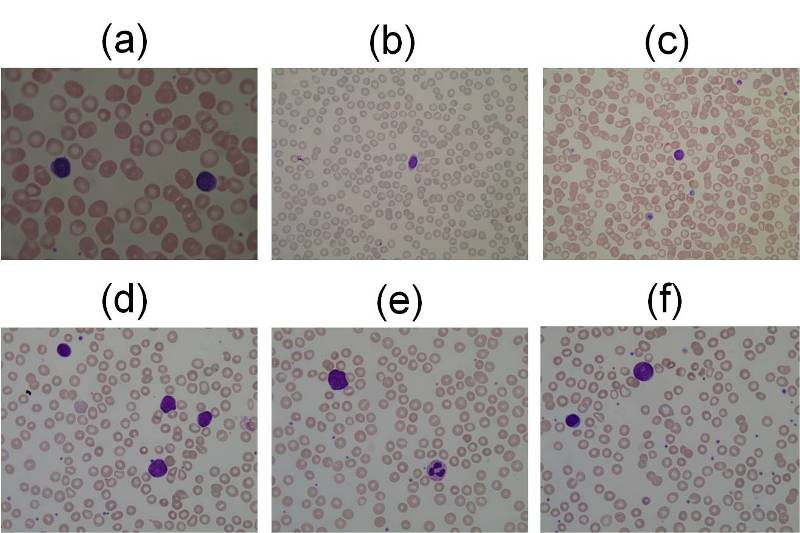
\includegraphics[width=5.8in]{../images/ALLIDB1.jpg}
\caption{Examples of the images contained in ALL-IDB1: healthy cells from non-ALL patients (a,b,c), probable lymphoblasts from ALL patients (d,e,f). }
\end{figure}

\textbf{annotation:} input image ''Im006\_1.jpg'' (a) and the related classification file ''Im006\_1.xyc'' reporting the coordinates of the centroids of probable ALL lymphoblasts (b).

\begin{figure}[H]
\begin{minipage}[b]{0.35\linewidth}
\centering
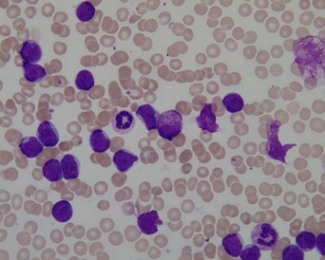
\includegraphics[width=55mm]{../images/Im006_1.jpg}
\subcaption{Im006\_1.jpg}
\label{fig:Im006.jpg}
\end{minipage}
\hfill
\begin{minipage}[b]{0.3\linewidth}
\centering
\lstinputlisting[breaklines]{../images/Im006\_1.xyc}
\subcaption{Im006\_1.xyc}
\label{fig:Im006.xyc}
\end{minipage}

\begin{minipage}[b]{0.35\linewidth}
\centering
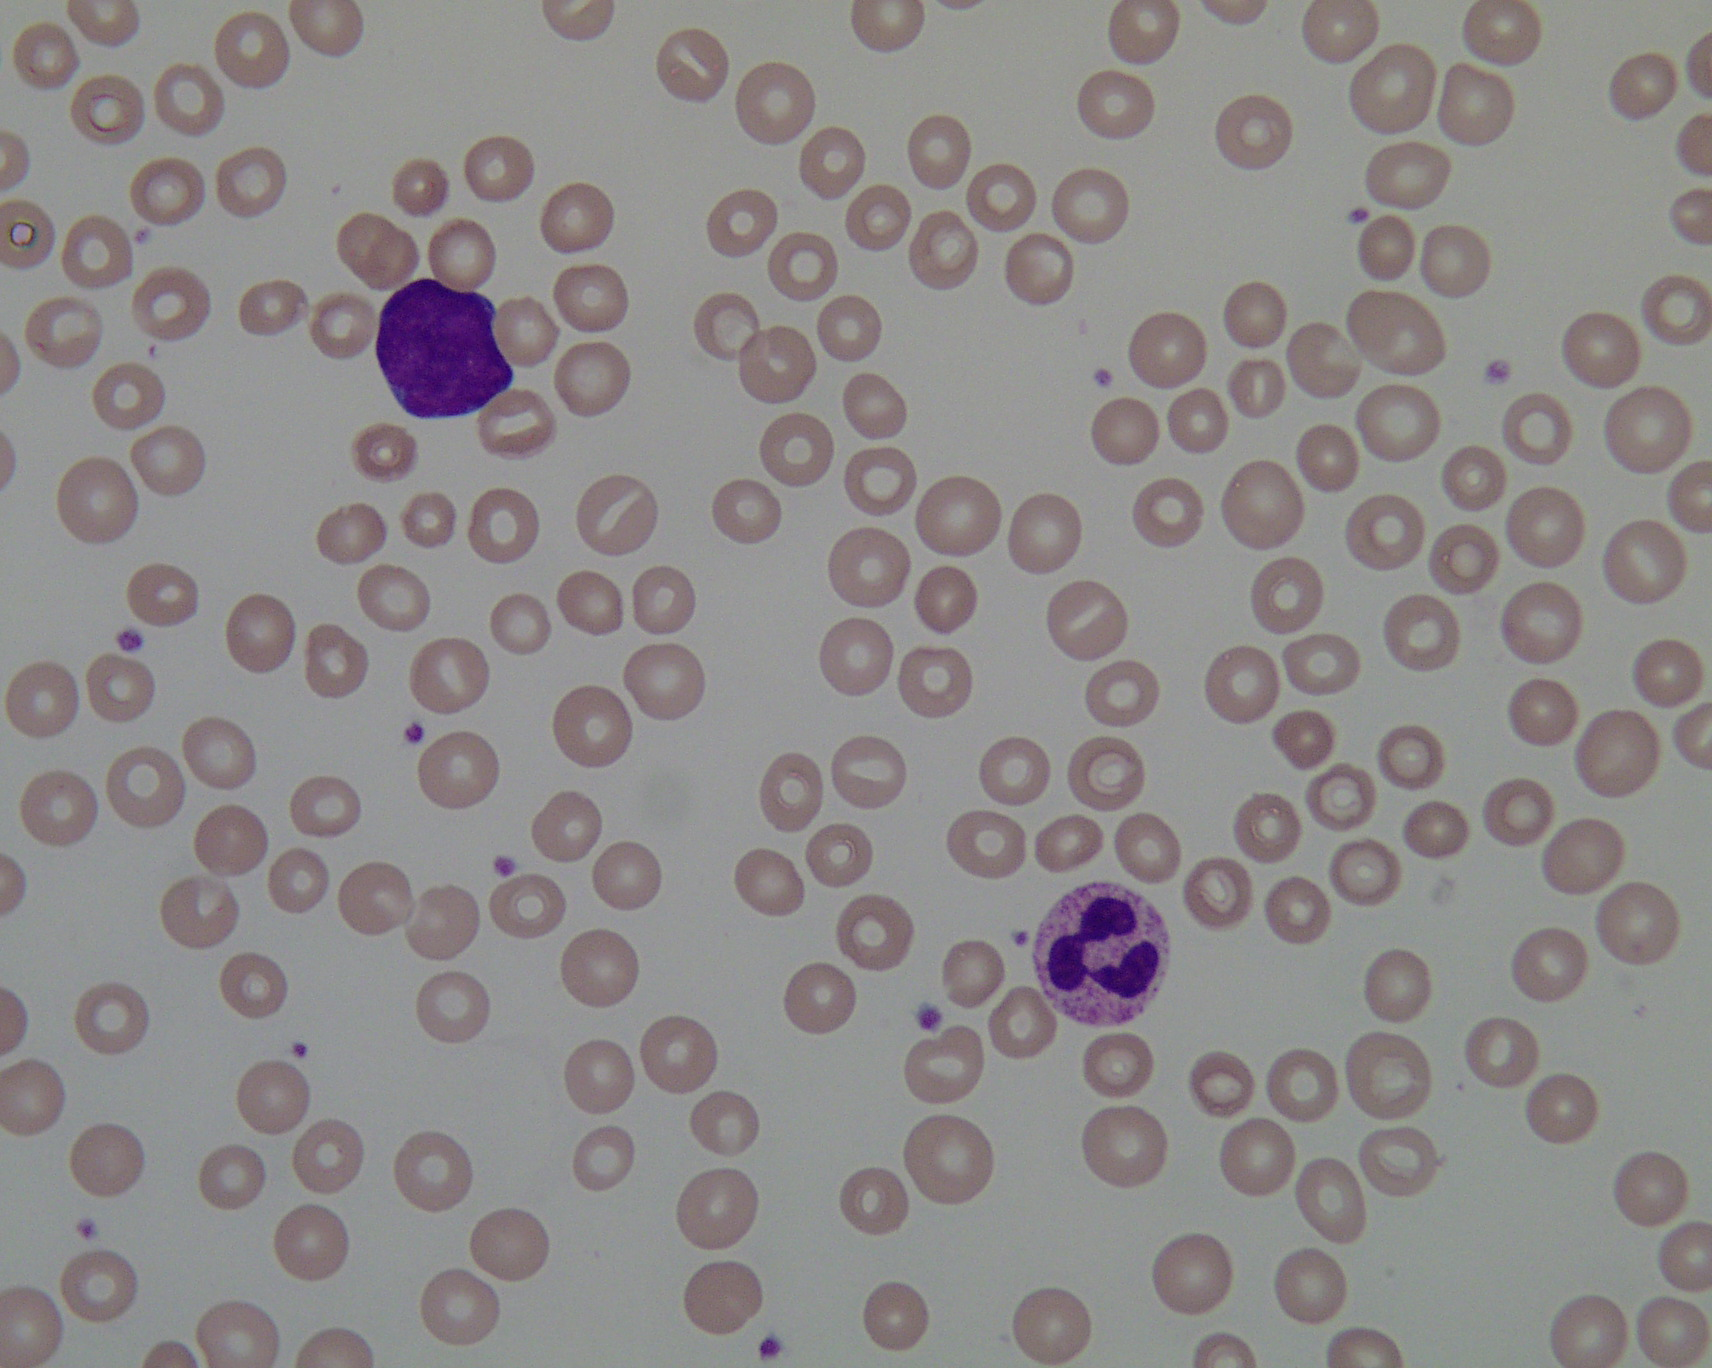
\includegraphics[width=55mm]{../images/Im033_1.jpg}
\subcaption{Im033\_1.jpg}
\label{fig:Im033.jpg}
\end{minipage}
\hfill
\begin{minipage}[b]{0.3\linewidth}
\centering
\lstinputlisting[breaklines]{../images/Im033\_1.xyc}
\subcaption{Im033\_1.xyc}
\label{fig:Im033.xyc}
\end{minipage}
\caption{Sample data from the ALL-IDB1 Database}
\end{figure}

The ALL-IDB1 image files are named with the notation ImXXX\_Y.jpg where XXX is a 3-digit integer counter and Y is a boolean digit equal to 0 if no blast cells are present, and equal to 1 if at least one blast cell is present in the image. All images labeled with Y=0 are from for healthy individuals, and all images labeled with Y=1 are from ALL patients. Each image file ImXXX\_Y.jpg (figure \ref{fig:Im006.jpg}, \ref{fig:Im033.jpg}) is associated with a text file ImXXX\_Y.xyc (figure \ref{fig:Im006.xyc}, \ref{fig:Im033.xyc}) reporting the coordinates of the centroids of the blast cells, if any.\\

If we plot the coordinates in the Img006\_1.xyc (figure \ref{fig:Im006.jpg}) file on the image Im006\_1.jpg (figure \ref{fig:Im006.xyc}) we get the figure \ref{fig:Im006.xyc.jpg}



\begin{figure}[H]
\centering
    \fbox{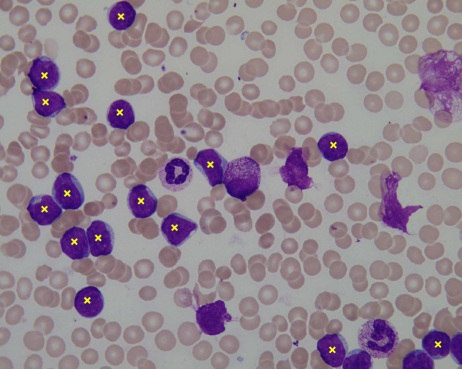
\includegraphics[width = 4in]{../images/img006.xyc.jpg}}
\caption{coordinates from Img006\_1.xyc plotted on Img006\_1.jpg}
\label{fig:Im006.xyc.jpg}
\end{figure}

\subsubsection{Dataset ALL-IDB1}
\hspace{\parindent}
This dataset has been created for testing the performances of classification systems. where the dataset has no segmentation information it contains only one information which is the presence of ALL lymphoblasts, the dataset is a collection of cropped area of interest of normal and blast cells that belongs to the ALL-IDB1 dataset as we can see in figure \ref{fig:ALL-IDB2}

\begin{figure}[H]
\centering
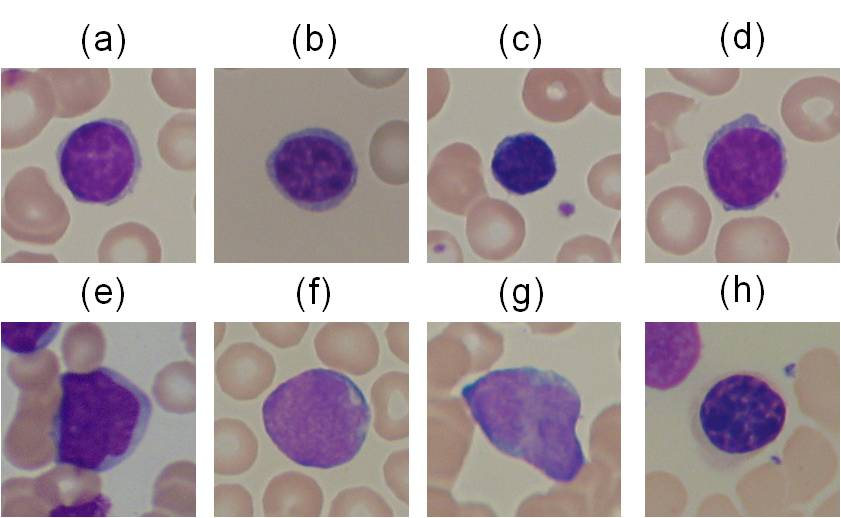
\includegraphics{../images/ALL-IDB2.jpg}
\caption{Examples of the images contained in ALL-IDB2: healthy cells from non-ALL patients (a-d), probable lymphoblasts from ALL patients (e-h).}
\label{fig:ALL-IDB2}
\end{figure}

\vspace{-0.14in}

The annotation of ALL-IDB2 is similar to the ALL-IDB1 but with no centroid coordinates. The ALL-IDB2 image files are named with the notation ImXXX\_Y.jpg where XXX is a progressive 3-digit integer and Y is a Boolean digit equal to 0 if the cell placed in the center of the image is not a blast cell, and equal to 1 if the cell placed in the center of the image is a blast cell. all images labeled with Y=0 are from for healthy individuals, and all images labeled with Y=1 are from ALL patients. 

\subsection{Broad Bio-image Benchmark Collection}
\hspace{\parindent}
The Broad Bio-image Benchmark Collection (BBBC) is a collection of freely downloadable microscopy image sets, cited in 450+ studies. In addition to the images themselves, each set includes a description of the biological application and some type of "ground truth" (expected results) \textsuperscript{\cite{ljosa2012annotated}}. The BBBC is organized by the Broad Institute's Imaging Platform.\

The dataset contains 54 image collections of various cell types, each collection has at least one of 6 ground truth types such as cell count, foreground / background, outlines of objects, biological labels, location and bounding boxes. in the sections below we describe each ground truth:

\subsubsection{Cell counts}
\hspace{\parindent}
In this case, the ground truth consists of the number of cells (or other objects) in each image, as counted by one or more humans. for example in BBBC1(Human HT29 colon-cancer cells) we have an image in figure \ref{fig:BBBC1} with the labels file in figure \ref{fig:BBBC001_Counts}:

\begin{figure}[H]
\begin{minipage}[c]{\linewidth}
\centering

\includegraphics[width = 2.2in]{../images/AS_09125_050118150001_A03f05d0.jpg}
\subcaption{AS\_09125\_050118150001\_A03f05d0.jpg}
\label{fig:BBBC1}
\end{minipage}

\begin{minipage}[c]{\linewidth}
\centering
\lstinputlisting[breaklines]{../images/BBBC001_v1_counts.txt}
\subcaption{BBBC001\_v1\_counts.txt}
\label{fig:BBBC001_Counts}
\end{minipage}
\caption{Sample data from the BBBC1 Database with counts Ground truth}
\end{figure}

in the figure \ref{fig:BBBC001_Counts} we can see the two counts performed by two experts, for the image \ref{fig:BBBC1} the first expert have found 241 cells but the second one found 257 cells.

\subsubsection{Foreground and background}
\hspace{\parindent}
In this case, a human produces a binary (black and white but in some cases thy use other colors) image the same size as the original image. Pixels that belong to the foreground (i.e., the cells or other objects) are white, and pixels that belong to the background are black. in the example below (figure \ref{fig:BBBC004_img} and \ref{fig:BBBC004_F}) we can see the image and the corresponding mask where the cells colored with blue and the background with black.

\begin{figure}[H]
\begin{minipage}[c]{0.4\linewidth}
\centering
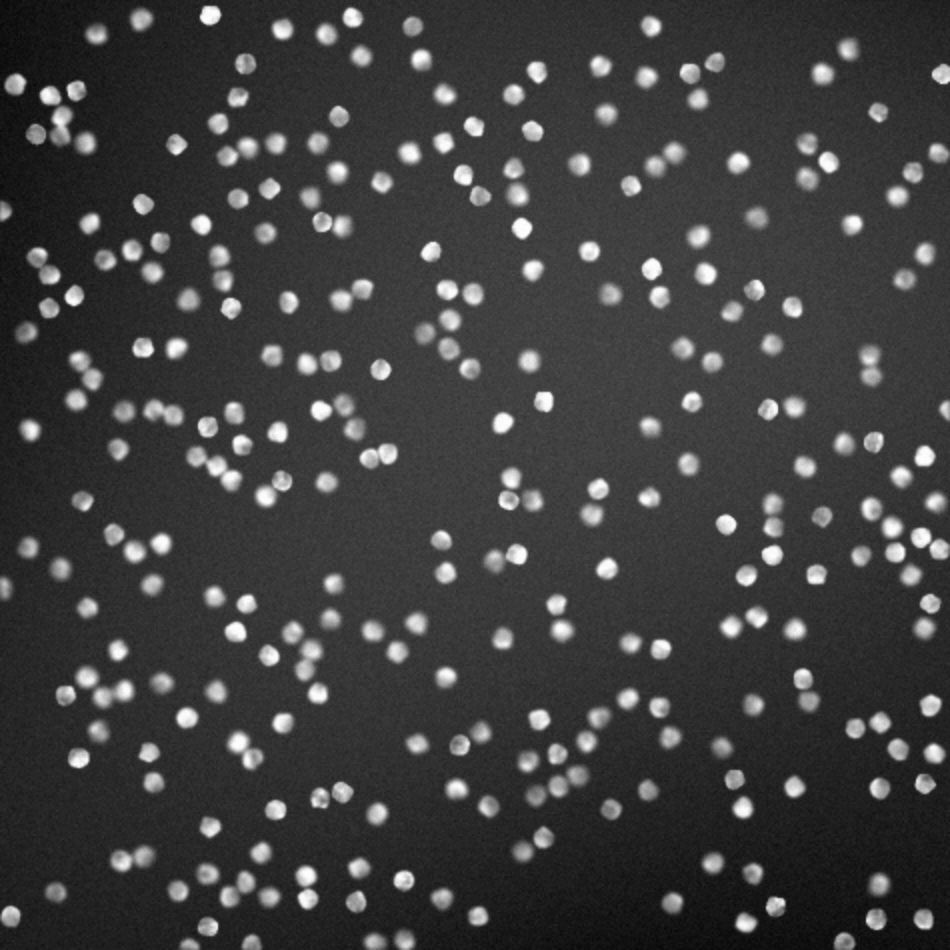
\includegraphics[width=50mm]{../images/BBBC4-1.jpg}
\subcaption{2Gray1.tif (image)}
\label{fig:BBBC004_img}
\end{minipage}
\hfill
\begin{minipage}[c]{0.4\linewidth}
\centering
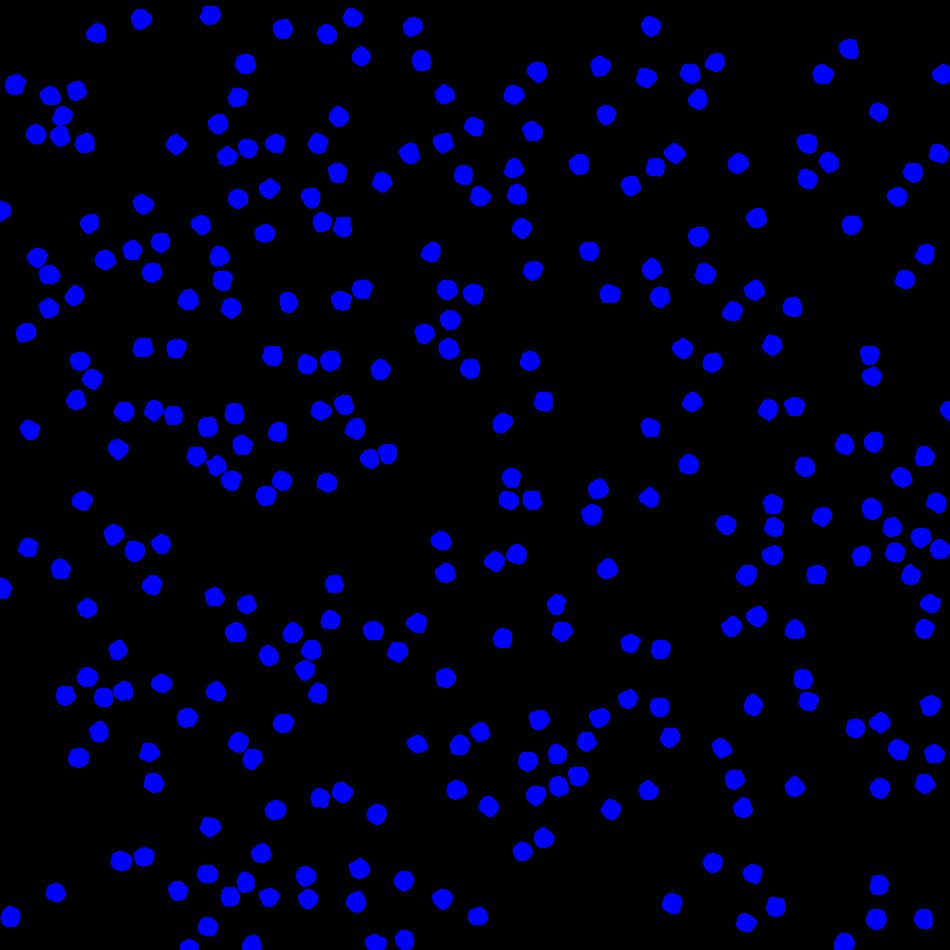
\includegraphics[width=50mm]{../images/BBBC4-1-F.jpg}
\subcaption{1.tif (mask)}
\label{fig:BBBC004_F}
\end{minipage}
\caption{Sample data from the BBBC4 Database with mask as ground truth}
\end{figure}

\subsubsection{Outlines of individual objects}
\hspace{\parindent}
In this case, a human outlines each cell in the image in order to indicate which pixels belong to which cell. The ground truth is provided as binary images, with black outlines on a white background.

\begin{figure}[H]
\begin{minipage}[c]{0.4\linewidth}
\centering
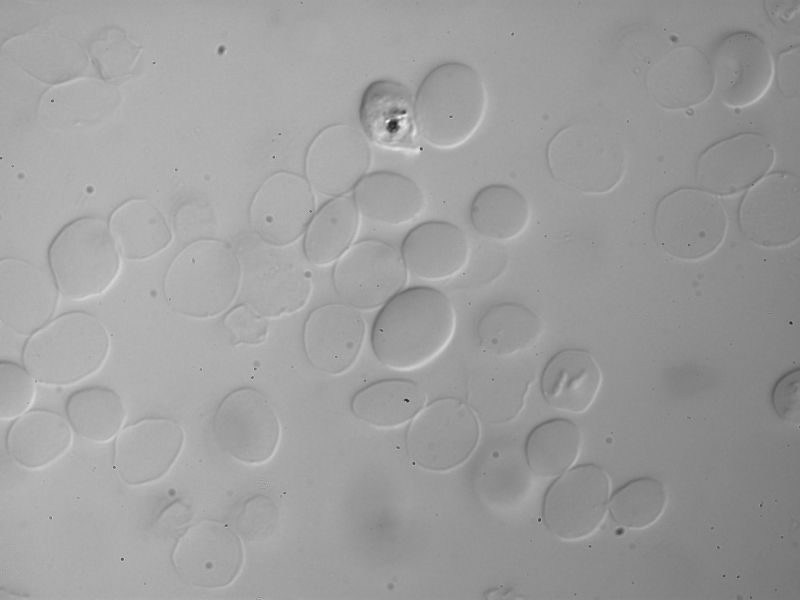
\includegraphics[width=50mm]{../images/48hr-001-DIC.jpg}
\subcaption{48hr-001-DIC.jpg (image)}
\label{fig:BBBC009_img}
\end{minipage}
\hfill
\begin{minipage}[c]{0.4\linewidth}
\centering
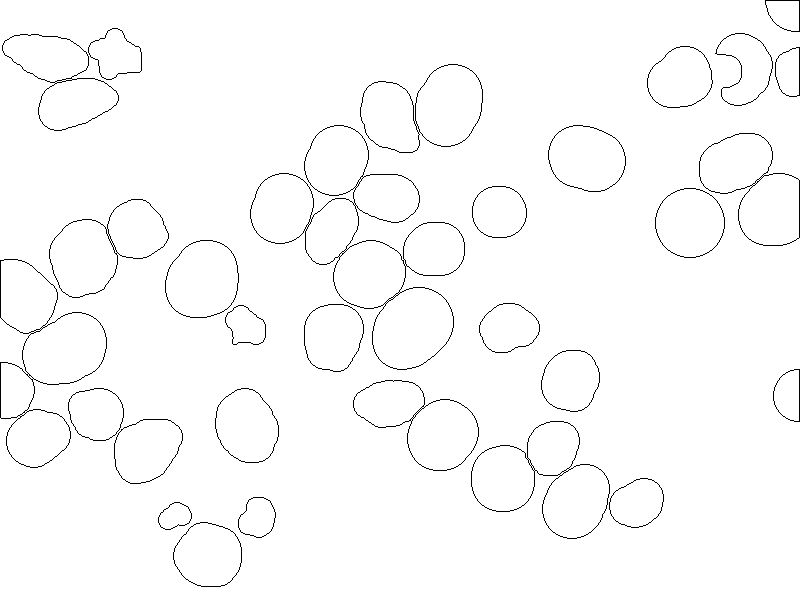
\includegraphics[width=50mm]{../images/48hr-001-DIC_.jpg}
\subcaption{48hr-001-DIC.jpg (edge mask)}
\label{fig:BBBC009_O}
\end{minipage}
\caption{Sample data from the BBBC9 Database with edge mask (outlines) as ground truth}
\end{figure}

\subsubsection{Biological labels}
\hspace{\parindent}
In these cases, the experiments have been prepared with control samples for which we know the expected biological result. The types of controls that are available dictate the type of statistic that can be calculated.

\subsubsection{Location}
\hspace{\parindent}
In this case, the ground truth consists of the X, Y, and optionally Z location of objects (typically their centroids similar to ALL-IDB1 Annotation \ref{fig:Im006.xyc.jpg}) .

\subsubsection{Bounding Boxes}
\hspace{\parindent}
Bounding boxes are rectangles completely enclosing an object.

\vspace{-0.1in}

\subsection{WBC Image Dataset : Fast and Robust Segmentation of White Blood Cell Images by Self-supervised Learning}
\hspace{\parindent}
This is two datasets of white blood cell (WBC) images used for “Fast and Robust Segmentation of White Blood Cell Images by Self-supervised Learning”, which can be used to evaluate cell image segmentation methods \textsuperscript{\cite{Zheng2018}}.\
This collection contains two datasets different from each other in terms of the image color, cell shape, background, etc. The ground truth segmentation results are manually sketched by domain experts, where the nuclei, cytoplasms and background including red blood cells are marked in white, gray and black respectively. 

\subsubsection{Dataset 1}
\hspace{\parindent}
Was obtained from Jiangxi Tecom Science Corporation \textsuperscript{\cite{2022_tecom-cn}}, China. It contains three hundred 120×120 images of WBCs and their color depth is 24 bits. The images were taken by a Motic Moticam Pro 252A optical microscope camera with a N800-D motorized auto-focus microscope.

\begin{figure}[H]
\centering
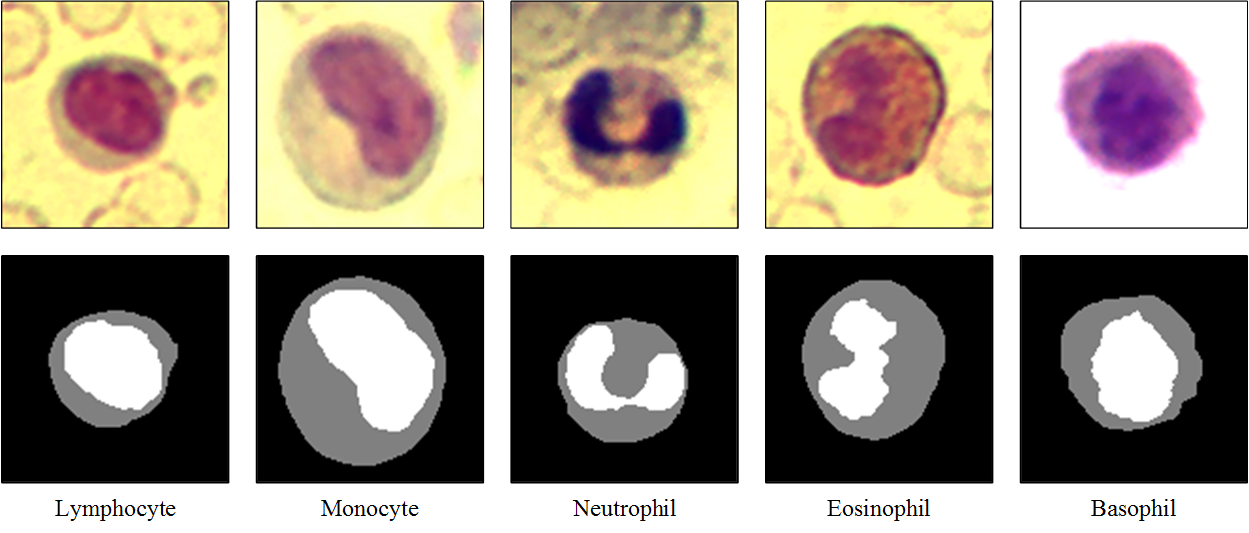
\includegraphics[width=5.2in]{../images/WBC_Dataset1.png}
\caption{Sample data from WBC\_Segmentaion Dataset 1}
\label{fig:WBC_Dataset1_sample}
\end{figure}

\subsubsection{Dataset 2}
Consists of one hundred 300×300 color images, which were collected from the Cella-Vision blog \textsuperscript{\cite{2022_cellavision}}. The cell images are generally purple and may contain many red blood cells around the white blood cells.

\begin{figure}[H]
\centering
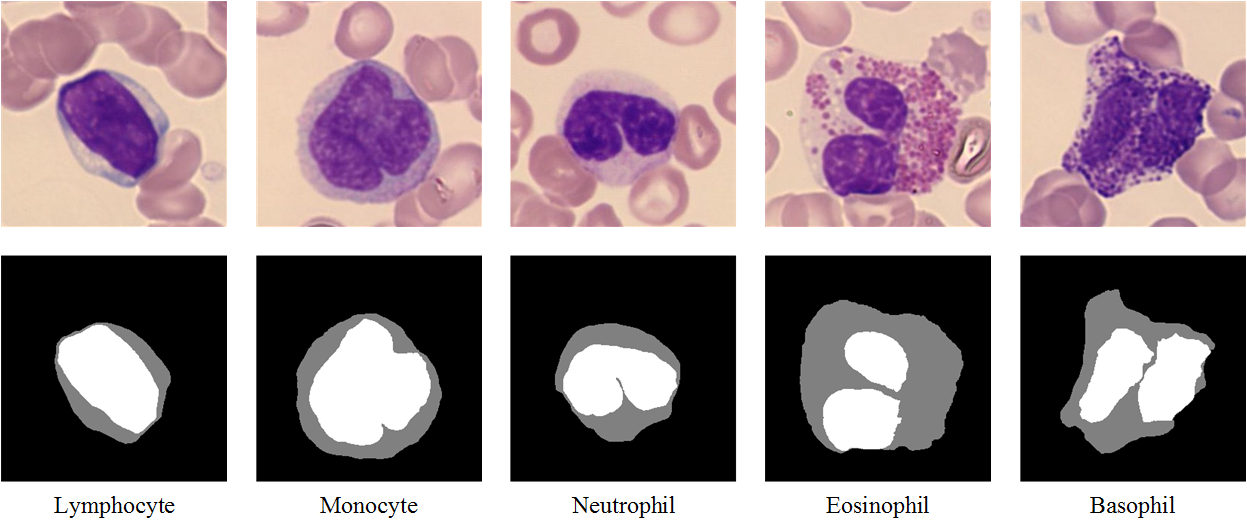
\includegraphics[width=5.2in]{../images/WBC_Dataset2.png}
\caption{Sample data from WBC\_Segmentaion Dataset 2}
\label{fig:WBC_Dataset2_sample}
\end{figure}

\subsection{Annotation}
\hspace{\parindent}
The class labels of each image in Dataset 1 and Dataset 2 are stored in csv files. The labels (1- 5) represent neutrophil, lymphocyte, monocyte, eosinophil and basophil, respectively.


\subsection{A large dataset of white blood cells containing cell locations and types, along with segmented nuclei and cytoplasm}
\hspace{\parindent}
The database is provided by \href{https://raabindata.com/free-data/#double-labeled-cropped-cells}{RabinData} and \textsuperscript{\cite{Kouzehkanan2022}} which divides on two separate datasets:

\subsubsection{Raabin-WBC Data}
\hspace{\parindent}
Contains 4 sub-Datasets:
\begin{itemize}
    \item \textbf{Double-labeled cropped cells} : Double-labeled cropped cells are also provided containing only five main classes including mature neutrophils, lymphocytes (small and large), eosinophils, monocytes, and basophils. 
    \item \textbf{Nucleus\_cytoplasm\_Ground truths} : in this sub-Dataset they prepared the ground truths of the cytoplasm and the nucleus for a proper number of cropped white blood cells. For this purpose, 1145 cropped images including 242 lymphocytes, 242 monocytes, 242 neutrophils, 201 eosinophils, and 218 basophils were randomly selected, and their ground truths were extracted by an expert.
    \item \textbf{Microscopic images were taken by the Olympus CX18 microscope and the Samsung Galaxy S5 camera and the 4th database with contain images taken by Zeiss microscope and the LG G3 camera } : in these two sub-Datasets. Corresponding to each microscopic image, a dictionary (json format) file containing the following information about that image was provided:
    \begin{itemize}
        \item Information about the blood elements in the image including their coordinates and labels.
        \item Information about the blood smears including staining method and the type of the disease.
        \item Information about the microscope includes the type of microscope and its magnification size.
        \item The type of camera used.
    \end{itemize}
\end{itemize}

\subsubsection{Raabin-Leukemia Data}
\hspace{\parindent}
Contains 4 sub-Datasets:
\begin{itemize}
    \item \textbf{Acute Lymphoblastic Leukemia}
    \item \textbf{Acute Myeloblastic Leukemia} 
    \item \textbf{Chronic Lymphocytic Leukemia}
    \item \textbf{Chronic Myelogenous Leukemia}
\end{itemize}
In each of these sub-Dataset, All samples were taken from patients who had referred to our collaborator medical laboratory (Takht-e Tavous Laboratory in Tehran, Iran). It should be notices Zeiss microscope and LG J3 smartphone camera had been used for imaging.

\subsection{BCCD}
\hspace{\parindent}
BCCD (Blood Cell Count and Detection) Dataset is a small-scale dataset for blood cells detection. The dataset contains a total of 364 (640x480) jpeg images with their annotations. The original data and annotations are from \href{https://github.com/cosmicad/dataset}{cosmicad} and \href{https://github.com/akshaylamba/all_CELL_data}{akshaylamba}.\\
In this project, the Faster R-CNN algorithm from keras-frcnn for Object Detection is used. From this dataset, nicolaschen1 developed two Python scripts to make preparation data (CSV file and images) for recognition of abnormalities in blood cells on medical images.

\begin{figure}[H]
\centering
    \fbox{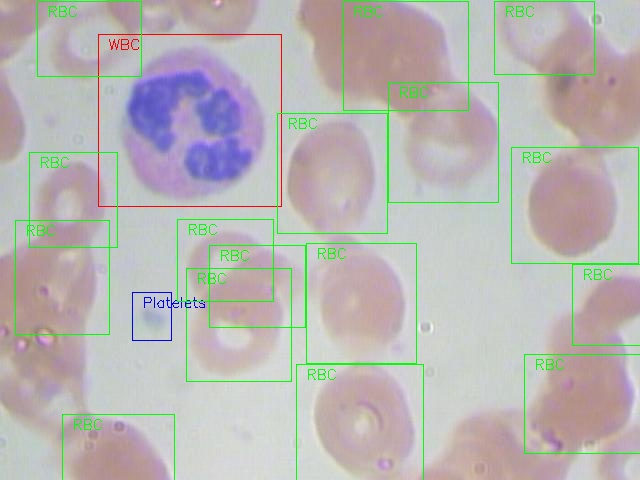
\includegraphics[width=4.2in]{../images/BBCD1.jpg}}
\caption{Sample data from BBCD}
\label{fig:BBCD1}
\end{figure}

In this database they use bounding boxes to locate the cells and each bounding box has the type of cell RBC or WBC and Platelets. they are using the VOC format as a database architecture.

\subsection{Dataset collections resume}
\hspace{\parindent}

\begin{table}[H]
\centering
\resizebox{\textwidth}{!}{%
\begin{tabular}{|c|c|ccc|c|c|}
\hline
\cellcolor[HTML]{FFFFFF}\textbf{\begin{tabular}[c]{@{}c@{}}Dataset\\ Name\end{tabular}} &
  \cellcolor[HTML]{FFFFFF}\textbf{\begin{tabular}[c]{@{}c@{}}Dataset\\ Size\end{tabular}} &
  \multicolumn{3}{c|}{\textbf{\begin{tabular}[c]{@{}c@{}}Type of cells\\ (RBC, WBC, Platelets)\end{tabular}}} &
  \cellcolor[HTML]{FFFFFF}\textbf{Type of annotation} &
  \cellcolor[HTML]{FFFFFF}\textbf{Description} \\ \hline
\cellcolor[HTML]{FFFFFF}ALL-IDB \textsuperscript{\cite{pm77-2n23-20}}&
  \cellcolor[HTML]{FFFFFF}108 &
  \multicolumn{1}{c|}{108 masks / 13 edges} &
  \multicolumn{1}{c|}{108 masks} &
  108 masks&
  \cellcolor[HTML]{FFFFFF}\begin{tabular}[c]{@{}c@{}}Location \\ (Centroid of cells)\end{tabular} &
  \cellcolor[HTML]{FFFFFF}\begin{tabular}[c]{@{}c@{}}Acute Lymphoblastic\\ Leukemia Image Database\\ for Image Processing\end{tabular} \\ \hline
\cellcolor[HTML]{FFFFFF}BBBC \textsuperscript{\cite{ljosa2012annotated}} &
  \cellcolor[HTML]{FFFFFF}Lots of subdatasets &
  \multicolumn{1}{c|}{X} &
  \multicolumn{1}{c|}{X} &
  X &
  \cellcolor[HTML]{FFFFFF}\begin{tabular}[c]{@{}c@{}}All types of\\ annotations\end{tabular} &
  \cellcolor[HTML]{FFFFFF}\begin{tabular}[c]{@{}c@{}}Broad Bioimage Benchmark\\ Collection\end{tabular} \\ \hline
\cellcolor[HTML]{FFFFFF}WBC Image Dataset &
  \cellcolor[HTML]{FFFFFF}400 &
  \multicolumn{1}{c|}{} &
  \multicolumn{1}{c|}{X} &
   &
  \cellcolor[HTML]{FFFFFF}\begin{tabular}[c]{@{}c@{}}Foreground and\\ Background (mask)\end{tabular} &
  \cellcolor[HTML]{FFFFFF}\begin{tabular}[c]{@{}c@{}}WBC Image Dataset : \\ Fast and Robust Segmentation\\ of White Blood Cell Images\\ by Self-supervized Learning\end{tabular} \\ \hline
    BCCD \textsuperscript{\cite{BCCD_Dataset}} &
  364 &
  \multicolumn{1}{c|}{} &
  \multicolumn{1}{c|}{x} &
   &
  Bounding boxes &
  Blood Cell Count and Detection \\ \hline
\end{tabular}%
}
\caption{Table that resumes datasets mentioned above}
\label{Table that resumes datasets mentioned above}
\end{table}


\section{Computer-assisted blood cell segmentation and counting review}

\subsection{Image Processing Approaches}
\hspace{\parindent}
Bhavnani et al. \textsuperscript{\cite{bhavnani2016segmentation}} have developed a method for segmenting and counting RBC (red blood cells), WBC (White blood cells) and platelets which is also called complete blood count (CBC), by using Otsu’s thresholding and morphological operations as a segmentation method, and for counting the are preforming a comparison between two methods: the watershed algorithm and Circular Hough Transform. The model takes an RGB image as an input apply some processing steps then uses Otsu's thresholding to extract RBC and WBC separately with different threshold values then apply the two algorithm to compare the results, the model has no image size constraint because it's based only on image processing techniques and needs a small database to select the threshold values for RBC and WBC in this article they used 20 images. In the Experiment phase they used ALLIDB Database which contains 108 images with 1712x1368 and 2592x1944 resolution.The CHT method is the best in terms of accuracy with 92.67\% but it has some weaknesses with overlapping cells and morphological abnormalities. In the other side the watershed method which is a little bit adapted with overlapping and touching cells had an accuracy of 91.07\%.\

Guiliang, FENG et al. \textsuperscript{\cite{guiliang2016microscopic}} have a developed an algorithm that segments and counts cell images based on image definition, a Discrete Cosine Transform (DCT) is applied, which is proposed by N. Ahmed and Rao in 1974 \textsuperscript{\cite{ahmed1974discrete}}. Instead of the traditional watershed approach, the DCT method showed better results in comparison.\

However, there is a drawback to this approach, because this algorithm depends on image definition it relies on well focused images, consequently, when the images are out of focus the segmentation and counting is not reliable. But despite that drawback, it achieved a relatively high accuracy of over 90\% which is better that the watershed method.\\

K. Sudha and P. Geetha \textsuperscript{\cite{SUDHA2020639}} have developed a two stage framework which will segment the leukocytes (a type of WBC) with an edge strength-based Grabcut method as a first stage, in the second stage will count the cells using the novel gradient circular hough transform (GCHT) method. the model takes and RGB image convert it to HSV color space to extract the S component where the WBCs are more clear then applies the edge strength-based location detection the results are fed to fine segmentation using Grabcut Algorithm which will output the edge segmentation mask, for the counting the mask will be fed to the proposed GCHT Algorithm. In the experiments phase they used ALL-IDB \textsuperscript{\cite{labati2011all}} and Cellavision \textsuperscript{\cite{Zheng2018}} datasets, after resizing the images to 256x256.\\
After the experiments the proposed method had reached an average segmentation accuracy of 99.32\% and a counting accuracy of 97.3\%.\\
The new GCHT method can segment touched cells and even overlapped cells.

\subsection{Machine Learning Approaches}
\hspace{\parindent}
Kimbahune et al. \textsuperscript{\cite{kimbahune2011blood}} have developed a method for segmenting and counting red blood cells (RBC) and white blood cells (WBC).
segmentation is done using Pulse-Coupled Neural Network (PCNN) and square tracing algorithm for contour tracing after de-noising it with PCNN combined with median filter, the counting is performed by scanning the image and using edge detection methods as square tracing algorithm. this method gave good results compared to state of art methods.\\
%this kimbahune article they didn't give any info about the database or the experimental results 

Carlos X. Hern{\'{a}}ndez et al. \textsuperscript{\cite{DBLP:journals/corr/abs-1802-10548}} have implemented a convolutional neural network (CNN) using a feature pyramid network (FPN) combined with a VGG style neural network for segmenting and counting of cells in a given microscopy image.\
The dataset they used is BBBC005 \textsuperscript{\cite{ljosa2012annotated}} from Broad Institute's Bio-image Benchmark Collection, which consists of 9600 images and each image is 696x520 pixels but they were scaled down to 256x192 for the purposes of their experiment.\

Out of the total 9600 images only 600 of the images which have a corresponding mask were used for the FPN training. And 100 of those were used for fast prototyping and a standard of 80-20 train/test split for the final models.\
On the other hand, the full 9600 images were used for the VGG network.
This approach achieved a relatively good accuracy of 81.75\% but with some failure cases such as:\
%the accuracy is calculated manually from the given results in the article
% 100 - (rmspe = np.sqrt(np.mean(np.square(((y_true - y_pred) / y_true)), axis=0)))

\begin{itemize}
  \item High cell overlap
  \item Irregular cell shapes
  \item bad focal planes.
\end{itemize}

Tran, Thanh and Minh et al. \textsuperscript{\cite{tran2019blood}} have developed a method for segmenting and counting RBC and WBCs by using the SegNet model initialised with weights from a pre-trained VGG-16 model, for the counting they first apply Distance transform with 4 different distance metrics, then they apply binary dilation. At the End, they apply the connected component labeling algorithm to count the number of separated cells in images mask. for the training they used 42 images from ALL-IDB1 \textsuperscript{\cite{labati2011all}} after they cropped them to decrease the computation time and memory usage and reduce the number of RBC compared to WBC the result images have a resolution of 360*480*3 (RGB), they used 29 images for training and 13 for testing ,the model had a segmentation accuracy of 89\% and counting accuracy of 93.3\% on RBC and accuracy of 100\% on WBC with the testing database which has the cropped images of RBC and WBC.\

On the first database with cropped images they had only few WBC but in this second database they have more WBC , the database 2 contains 108 only WBC images with the same size of database 1 360*480*3, they augmented the training dataset from 76 to 380 and used 32 images for testing, this second model focus only on the WBC which will increase the segmentation accuracy to 98.5\%, and have a counting accuracy of 97.29\%. The counting accuracy have decreased because of the clumped cells which is the weakness of this model.\\

Yan Kong et al. \textsuperscript{\cite{Kong:20}} have developed a two-stage framework using parallel modified U-Nets together with seed guided water-mesh algorithm for automatic segmentation and yeast cells counting which is used to observe the living conditions and survival of yeast cells under experimental conditions.\

The cell images used in this study were captured by Olympus IX83 (Olympus Life Sciences, Tokyo, Japan) inverted microscope. They manually selected 20 raw DIC (differential interference contrast) images which contained a number of yeast cells and the annotations were done manually by laboratory technicians, they then obtain 40 images, 20 masked annotation images and the other 20 is center annotation images of yeast cells.\

After splitting images into tiles of size 224x224 with a step stride of 65 and 33 pixels for the horizontal and vertical direction, respectively. They got 4360 raw image tiles and the corresponding center annotation and masked annotation images, from that set 3310 tiles were randomly selected as the training data set and rest was a validation set.

The raw test DIC images used in this study were sized approximately 1002x1998 pixels, but they were resized into 1092x2084 pixels so that each DIC image could be split into a grid of 8x16 image blocks. The image blocks were then fed into modified U-Net.

This method achieved a precision of over 99.74\% and an average recall rate of 99.35\%. however, there is a limitation using this approach, which is the detection of small objects.\\

Shahzad, Muhammad et al. \textsuperscript{\cite{shahzad2020robust}} have developed a custom convolutional encoder-decoder framework along with VGG-16 as the pixel-level feature extraction model to address the problem of whole-slide cell segmentation using the semantic segmentation approach. Their proposed framework works as follows: First, all the original images along with manually generated ground truth masks of each blood cell type are passed through the pre-processing stage. In the pre-processing stage, pixel-level labeling, RGB to gray-scale conversion of masked image and pixel fusing, and unity mask generation are performed. After that, VGG16 is loaded into the system, which acts as a pre-trained pixel-level feature extraction model. Finally, the training process is initiated on the proposed model.

They used ALL-IDB1 as their baseline dataset which consists of 108 whole-slide blood cell images, 59 (2592x1944) images were from healthy individuals and 49 (1712x1368) images from acute lymphoblastic leukemia (ALL) patients.

This approach achieved a class-wise accuracy of 97.45\%, 93.34\%, and 85.11\% for RBCs, WBCs, and platelets, respectively, while global and mean accuracy remain 97.18\% and 91.96\%, respectively.\\

Overton, Toyah and Tucker, Allan \textsuperscript{\cite{10.1007/978-3-030-44584-3_31}} have developed a method which segments and counts IDP (Internally Displaced people) and erythrocytes (red blood cells) using DO-U-Net (Dual Output U-Net) which outputs a segmentation mask and an edge mask then they subtract them to get rid of the overlapping and the touching problem, the model trains on extremely small datasets (10 images) and gives a high segmentation accuracy, They selected 10 images of 108 from ALL-IDB dataset for training the model, the model takes images with a resolution of 188x188 and outputs a segmentation mask and edge mask of lower resolution 100x100, the experiments results have given an accuracy of 98.31\% on a 5 randomly selected images from ALL-IDB, for the IDP they had 98.69\% for fixed resolution images and 94.66\% for scale-invariant satellite images.\\

Li, Dongming et al. \textsuperscript{\cite{li2021robust}} have developed a method for segmenting blood cells by combining neural ordinary differential equations (NODEs) with U-Net networks to improve the accuracy of image segmentation. In order to study the effect of ODE-solve on the speed and accuracy of the network, the ODE-block module was added to the nine convolutional layers in the U-Net network. Firstly, blood cell images are pre-processed to enhance the contrast between the regions to be segmented; secondly, the same dataset was used for the training set and testing set to test segmentation results. Then they select the location where the ordinary differential equation block (ODE-block) module is added, select the appropriate error tolerance, and balance the calculation time and the segmentation accuracy, in order to exert the best performance.\

Finally, the error tolerance of the ODE-block is adjusted to increase the network depth, and the training NODEs-UNet network model is used for cell image segmentation. 

The experiment dataset for this model was provided by the Center for Medical Image and Signal Processing (MISP) and the Department of Pathology, Isfahan University of Medical Sciences \textsuperscript{\cite{sarrafzadeh2014selection}}. MISP.rar contains 148 clear blood cell smear images with a size of 775x519 pixels. They picked up appropriate areas for convenient network training, then cropped 100 blood cell images with a size of 256x256 pixels by selecting a suitable area. To ensure the accuracy of the training model, they retained 20 images as the testing set and used the remaining 80 images to increase the dataset to 800 by data augmentation. Besides, they used a ratio of 3 : 1 as the training set and the validation set.

Using this approach to segment blood cell images in the testing set, it can achieve 95.3\% pixel accuracy and 90.61\% mean intersection over union. By comparing the U-Net and ResNet networks, the pixel accuracy of this network model is increased by 0.88\% and 0.46\%, respectively, and the mean intersection over union is increased by 2.18\% and 1.13\%, respectively.

\section{Comparative study}

\begin{table}[H]
\centering
\resizebox{\textwidth}{!}{%
\begin{tabular}{|l|cc|c|cc|c|c|}
\hline
\rowcolor[HTML]{FFFFFF} 
\multicolumn{1}{|c|}{\cellcolor[HTML]{FFFFFF}\textbf{Reference}} &
  \multicolumn{1}{c|}{\cellcolor[HTML]{FFFFFF}\textbf{\begin{tabular}[c]{@{}c@{}}Segmentation\\ Approach\end{tabular}}} &
  \textbf{\begin{tabular}[c]{@{}c@{}}Counting\\ Approach\end{tabular}} &
  \textbf{\begin{tabular}[c]{@{}c@{}}Image\\ Size\end{tabular}} &
  \multicolumn{1}{c|}{\cellcolor[HTML]{FFFFFF}\textbf{\begin{tabular}[c]{@{}c@{}}Segmentation\\ Accuracy\end{tabular}}} &
  \textbf{\begin{tabular}[c]{@{}c@{}}Counting\\ Accuracy\end{tabular}} &
  \textbf{\begin{tabular}[c]{@{}c@{}}Database\\ Size\end{tabular}} &
  \textbf{\begin{tabular}[c]{@{}c@{}}Database\\ Name\end{tabular}} \\ \hline
\rowcolor[HTML]{FFFFFF} 
  \textbf{\begin{tabular}[c]{@{}l@{}}Kimbahune\\ et al. \textsuperscript{\cite{kimbahune2011blood}} \end{tabular}} &
  \multicolumn{1}{c|}{\cellcolor[HTML]{FFFFFF}PCNN} &
  Square tracing method &
  N/A &
  \multicolumn{1}{c|}{\cellcolor[HTML]{FFFFFF}N/A} &
  N/A &
  N/A &
  N/A \\ \hline
\rowcolor[HTML]{FFFFFF} 
  \textbf{\begin{tabular}[c]{@{}l@{}}Guiliang, FENG\\ et al. \textsuperscript{\cite{guiliang2016microscopic}} \end{tabular}} &
  \multicolumn{2}{c|}{\cellcolor[HTML]{FFFFFF}Discrete Cosine Transform (DCT)} &
  N/A &
  \multicolumn{2}{c|}{\cellcolor[HTML]{FFFFFF}90\%} &
  N/A &
  N/A \\ \hline
\rowcolor[HTML]{FFFFFF} 
  \textbf{\begin{tabular}[c]{@{}l@{}}Bhavnani\\ et al \textsuperscript{\cite{bhavnani2016segmentation}} \end{tabular}} &
  \multicolumn{1}{c|}{\cellcolor[HTML]{FFFFFF}\begin{tabular}[c]{@{}c@{}}OTsu's thresholding \\ and morphological\\ operations\end{tabular}} &
  \begin{tabular}[c]{@{}c@{}}1-Circular Hough\\ Transfer\\ 2-Watershed Algorithm\end{tabular} &
  \begin{tabular}[c]{@{}c@{}}2594x1944\\ 1712x1368\end{tabular} &
  \multicolumn{2}{c|}{\cellcolor[HTML]{FFFFFF}\begin{tabular}[c]{@{}c@{}}1- 92.67\%\\ 2- 91.07\%\end{tabular}} &
  20 / 108 &
  ALLIDB \\ \hline
\rowcolor[HTML]{FFFFFF} 
  \textbf{\begin{tabular}[c]{@{}l@{}}Carlos\\ et al. \textsuperscript{\cite{DBLP:journals/corr/abs-1802-10548}} \end{tabular}} &
  \multicolumn{2}{c|}{\cellcolor[HTML]{FFFFFF}\begin{tabular}[c]{@{}c@{}}FPN combined with VGG style\\ neural network\end{tabular}} &
  256x196 &
  \multicolumn{1}{c|}{\cellcolor[HTML]{FFFFFF}95\%} &
   &
  80 / 20 &
  BBBC005 \\ \hline
\rowcolor[HTML]{FFFFFF} 
  \textbf{\begin{tabular}[c]{@{}l@{}}Tran, Thanh \\ and\\ Minh et al. \textsuperscript{\cite{tran2019blood}} \end{tabular}} &
  \multicolumn{1}{c|}{\cellcolor[HTML]{FFFFFF}\begin{tabular}[c]{@{}c@{}}SegNet with weights\\ from a pre-trained\\ VGG-16\end{tabular}} &
  \begin{tabular}[c]{@{}c@{}}Distance Transform\\ and connected\\ component labeling\\ algorithm\end{tabular} &
  \begin{tabular}[c]{@{}c@{}}360x480x3\\ (RGB)\end{tabular} &
  \multicolumn{1}{c|}{\cellcolor[HTML]{FFFFFF}98.5\%} &
  97.29\% &
  380 / 32 &
  ALL-IDB1 \\ \hline
\rowcolor[HTML]{FFFFFF} 
  \textbf{\begin{tabular}[c]{@{}l@{}}K. Sudha and\\ P. Geetha \textsuperscript{\cite{SUDHA2020639}} \end{tabular}} &
  \multicolumn{1}{c|}{\cellcolor[HTML]{FFFFFF}\begin{tabular}[c]{@{}c@{}}Edge strength-based\\ Grabcut\end{tabular}} &
  \begin{tabular}[c]{@{}c@{}}Gradient Circular\\ Hough Transform\end{tabular} &
  256x256 &
  \multicolumn{1}{c|}{\cellcolor[HTML]{FFFFFF}99.32\%} &
  97.3\% &
   &
  ALL-IDB \\ \hline
\rowcolor[HTML]{FFFFFF} 
\textbf{\begin{tabular}[c]{@{}l@{}}Yan Kong\\ et al. \textsuperscript{\cite{Kong:20}} \end{tabular}} &
  \multicolumn{1}{c|}{\cellcolor[HTML]{FFFFFF}\begin{tabular}[c]{@{}c@{}}Two parallel\\ modified U-Nets\end{tabular}} &
  \begin{tabular}[c]{@{}c@{}}Seed Guided Water-\\ Mesh Algorithm\end{tabular} &
  224x224 &
  \multicolumn{2}{c|}{\cellcolor[HTML]{FFFFFF}96\%} &
  3310 / 1050 &
  Self Annotated \\ \hline
\textbf{\begin{tabular}[c]{@{}l@{}}Shahzad \\ et al. \textsuperscript{\cite{shahzad2020robust}} \end{tabular}} &
  \multicolumn{1}{c|}{\begin{tabular}[c]{@{}c@{}}Custom encoder-decoder\\ framework with VGG-16\end{tabular}} &
  N/A &
  \begin{tabular}[c]{@{}c@{}}2594x1944\\ 1712x1368\end{tabular} &
  \multicolumn{1}{c|}{\begin{tabular}[c]{@{}c@{}}97.45\%\\ 93.34\%\end{tabular}} &
  N/A &
  108 &
  ALL-IDB1 \\ \hline
\rowcolor[HTML]{FFFFFF} 
\textbf{\begin{tabular}[c]{@{}l@{}}Overton, Toyah\\ and\\ Tucker, Allan \textsuperscript{\cite{10.1007/978-3-030-44584-3_31}} \end{tabular}} &
  \multicolumn{1}{c|}{\cellcolor[HTML]{FFFFFF}DO-U-Net} &
  \begin{tabular}[c]{@{}c@{}}Marching Squares\\ Algorithm\end{tabular} &
  188x188 &
  \multicolumn{1}{c|}{\cellcolor[HTML]{FFFFFF}98.31\%} &
   &
  10 / 5 &
  ALL-IDB1 \\ \hline
\end{tabular}%
}
\caption{Table that represents a comparative study of previous methods}
\label{Table that represents a comparative study of previous methods}
\end{table}


We can see in the table \ref{table:comparative-study-state-of-art} each method with the approach they used, the accuracy that they achieved and the type of cells that they are  targeting.

\section{Conclusion}
\vspace{0.1in}
\hspace{\parindent}
First in this chapter, we explored all the available datasets and their annotations. Later, we saw the diversity of state of the art methods where most approaches have used deep learning as a segmentation method paired with multiple image processing methods for counting blood cells.

%we decided to work with the updated ALL-IDB1 dataset which has 13 RBC edges and masks, 108 WBC, Platelets Masks and 13 RBC images which has the count information, but the WBC and Platelets donthave the count information where we had to use manual count and algorithms to find the count information for these images.

%after we studied these articles we've chosen the article of Overton \textsuperscript{\cite{10.1007/978-3-030-44584-3_31}} because of the performance and optimisation of their segmentation model and we applied the same idea on the SegNet model, and for the counting methods we took the 3 of the most used methods to compare between them.

\newpage

\section{Introduction}
\hspace*{0.16in}

\section{ALL-IDB}

ALL-IDB (Acute Lymphoblastic Leukemia Image Database for Image Processing) \textsuperscript{\cite{labati2011all}} is a public and free dataset, specifically designed for the evaluation and the comparison of algorithms for segmentation and image classification. The database focus on Acute Lymphoblastic Leukemia (ALL), Acute is a type of blood cancer that starts in white blood cells in bone marrow, the soft inner part of bones. It develops from immature lymphocytes, a kind of white blood cell that’s key to immune system.\textsuperscript{\cite{Annie_Stuart_What_2022_webmd}}.\\

Each image in the dataset, Contains classification/position of ALL lymphoblasts is provided by expert oncologists. A lymphoblast is a modified naive lymphocyte with altered cell morphology. It occurs when the lymphocyte is activated by an antigen.\\

The images of the dataset has been captured with an optical laboratory microscope coupled with a Canon PowerShot G5 camera. All images are in JPG format with 24 bit color depth, resolution 2592 x 1944. the ALL-IDB devides on two Datasets ALL-IDB1 and ALL-IDB2.\\

\subsection{Dataset ALL-IDB1}

The ALL-IDB1 can be used for segmentation or classification with image processing methods or Artificial intelligence models. The dataset is composed of 108 images collected during September, 2005. It contains about 39000 blood elements, where the lymphocytes has been labeled by expert oncologists.

\begin{figure}[H]
\centering
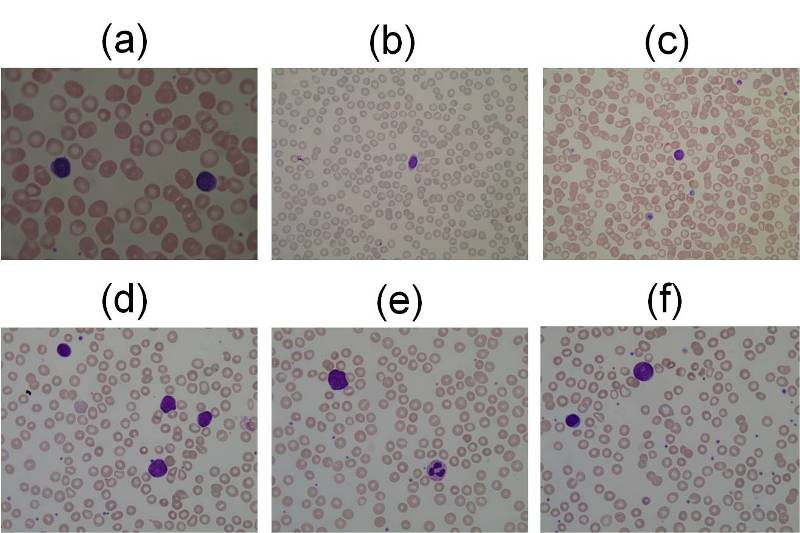
\includegraphics{../images/ALLIDB1.jpg}
\caption{Examples of the images contained in ALL-IDB1: healthy cells from non-ALL patients (a,b,c), probable lymphoblasts from ALL patients (d,e,f). }
\end{figure}


\textbf{annotation:} input image ''Im006\_1.jpg'' (a) and the related classification file ''Im006\_1.xyc'' reporting the coordinates of the centroids of probable ALL lymphoblasts (b).



\begin{figure}[H]
\begin{minipage}[b]{0.35\linewidth}
\centering
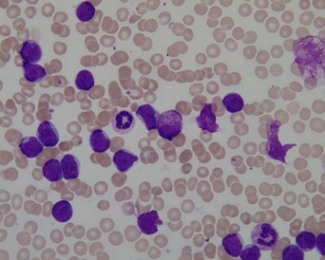
\includegraphics{../images/Im006_1.jpg}
\subcaption{Im006\_1.jpg}
\label{fig:Im006.jpg}
\end{minipage}
\hfill
\begin{minipage}[b]{0.3\linewidth}
\centering
\lstinputlisting[breaklines]{../images/Im006\_1.xyc}
\subcaption{Im006\_1.xyc}
\label{fig:Im006.xyc}
\end{minipage}

\begin{minipage}[b]{0.35\linewidth}
\centering
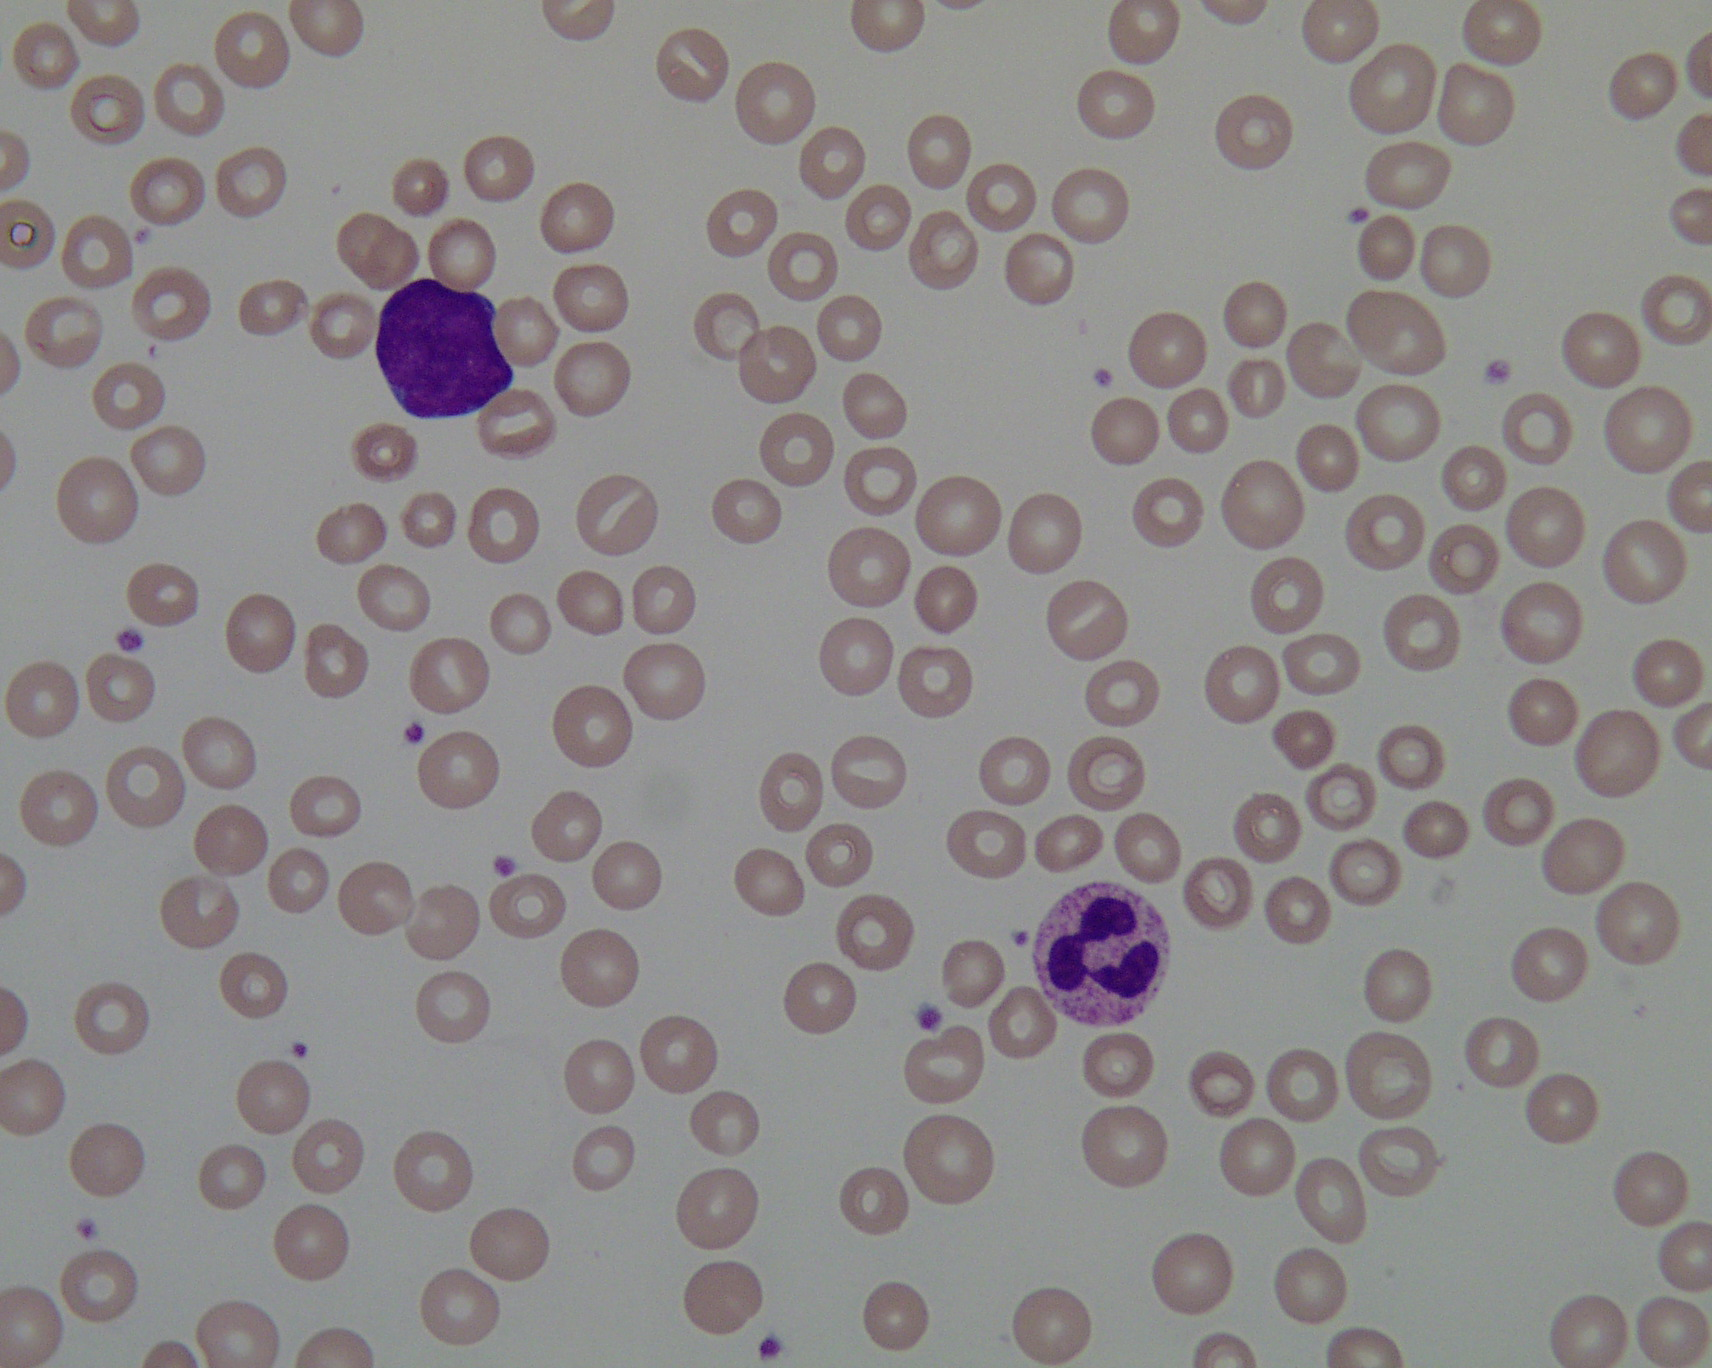
\includegraphics[width=57mm]{../images/Im033_1.jpg}
\subcaption{Im033\_1.jpg}
\label{fig:Im033.jpg}
\end{minipage}
\hfill
\begin{minipage}[b]{0.3\linewidth}
\centering
\lstinputlisting[breaklines]{../images/Im033\_1.xyc}
\subcaption{Im033\_1.xyc}
\label{fig:Im033.xyc}
\end{minipage}
\caption{Sample data from the ALL-IDB1 Database}
\end{figure}

The ALL-IDB1 image files are named with the notation ImXXX\_Y.jpg where XXX is a 3-digit integer counter and Y is a boolean digit equal to 0 if no blast cells are present, and equal to 1 if at least one blast cell is present in the image. All images labeled with Y=0 are from for healthy individuals, and all images labeled with Y=1 are from ALL patients. Each image file ImXXX\_Y.jpg (figure \ref{fig:Im006.jpg}, \ref{fig:Im033.jpg}) is associated with a text file ImXXX\_Y.xyc (figure \ref{fig:Im006.xyc}, \ref{fig:Im033.xyc}) reporting the coordinates of the centroids of the blast cells, if any. \\

if we plot the coordinates in the Img006\_1.xyc (figure \ref{fig:Im006.jpg}) file on the image Im006\_1.jpg (figure \ref{fig:Im006.xyc}) we get the figure \ref{fig:Im006.xyc.jpg}

\begin{figure}[H]
\centering
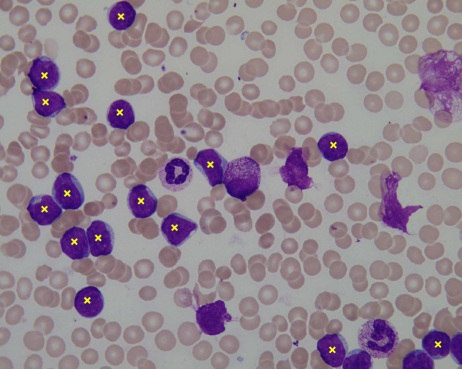
\includegraphics{../images/img006.xyc.jpg}
\caption{coordinates from Img006\_1.xyc ploted on Img006\_1.jpg}
\label{fig:Im006.xyc.jpg}
\end{figure}

\newpage

\subsection{Dataset ALL-IDB1}

This dataset has been created for testing the performances of classification systems. where the dataset has no segmentation information it contains only one information wich is the presence of ALL lymphoblasts, the dataset is a collection of cropped area of interest of normal and blast cells that belongs to the ALL-IDB1 dataset as we can see in figure \ref{fig:ALL-IDB2}


\begin{figure}[H]
\centering
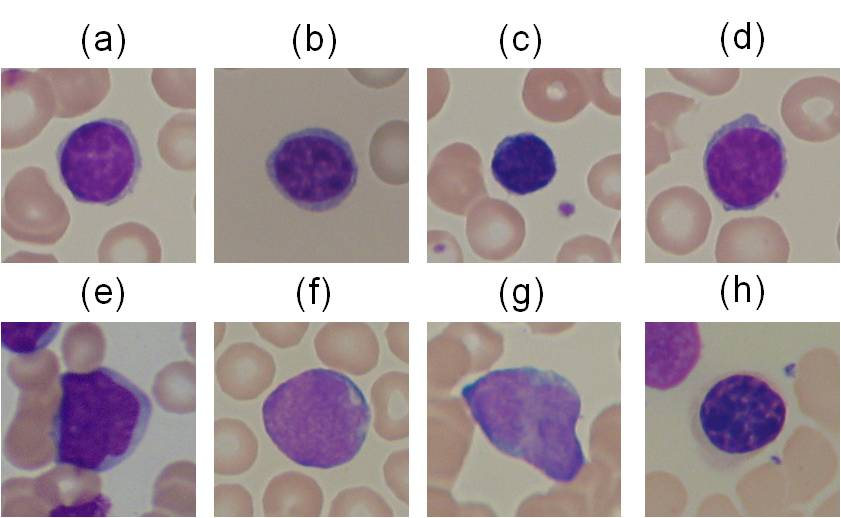
\includegraphics{../images/ALL-IDB2.jpg}
\caption{Examples of the images contained in ALL-IDB2: healthy cells from non-ALL patients (a-d), probable lymphoblasts from ALL patients (e-h).}
\label{fig:ALL-IDB2}
\end{figure}


The annotation of ALL-IDB2 is similar to the ALL-IDB1 but with no centroid coordinates. The ALL-IDB2 image files are named with the notation ImXXX\_Y.jpg where XXX is a progressive 3-digit integer and Y is a boolean digit equal to 0 if the cell placed in the center of the image is not a blast cell, and equal to 1 if the cell placed in the center of the image is a blast cell. all images labeled with Y=0 are from for healthy individuals, and all images labeled with Y=1 are from ALL patients. 

\newpage 

\section{Broad Bioimage Benchmark Collection}

The Broad Bioimage Benchmark Collection (BBBC) is a collection of freely downloadable microscopy image sets, cited in 450+ studies. In addition to the images themselves, each set includes a description of the biological application and some type of "ground truth" (expected results) \textsuperscript{\cite{ljosa2012annotated}}. The BBBC is organized by the Broad Institute's Imaging Platform.\\

The dataset contains 54 image collections of various cell types, each collection has at least one of 6 ground truth types such as cell count, foreground / background, outlines of objects, biological labels, location and bounding boxes. in the sections below we describe each ground truth:
\subsection{Cell counts}
In this case, the ground truth consists of the number of cells (or other objects) in each image, as counted by one or more humans. for example in BBBC1(Human HT29 colon-cancer cells) we have an image in figure \ref{fig:BBBC1} with the labels file in figure \ref{fig:BBBC001_Counts}:

\begin{figure}[H]
\begin{minipage}[c]{\linewidth}
\centering

\includegraphics[width=60mm]{../images/AS_09125_050118150001_A03f05d0.jpg}
\subcaption{AS\_09125\_050118150001\_A03f05d0.jpg}
\label{fig:BBBC1}
\end{minipage}

\begin{minipage}[c]{\linewidth}
\centering
\lstinputlisting[breaklines]{../images/BBBC001_v1_counts.txt}
\subcaption{BBBC001\_v1\_counts.txt}
\label{fig:BBBC001_Counts}
\end{minipage}
\caption{Sample data from the BBBC1 Database with counts Ground truth}
\end{figure}


in the figure \ref{fig:BBBC001_Counts} we can see the two counts performed by two experts, for the image \ref{fig:BBBC1} the first expert have found 241 cells but the second one found 257 cells.

\subsection{Foreground and background}

In this case, a human produces a binary (black and white but in some cases thy use other colors) image the same size as the original image. Pixels that belong to the foreground (i.e., the cells or other objects) are white, and pixels that belong to the background are black. in the example below (figure \ref{fig:BBBC004_img} and \ref{fig:BBBC004_F}) we can see the image and the corresponding mask where the cells colored with blue and the background with black.

\begin{figure}[H]
\begin{minipage}[c]{0.4\linewidth}
\centering
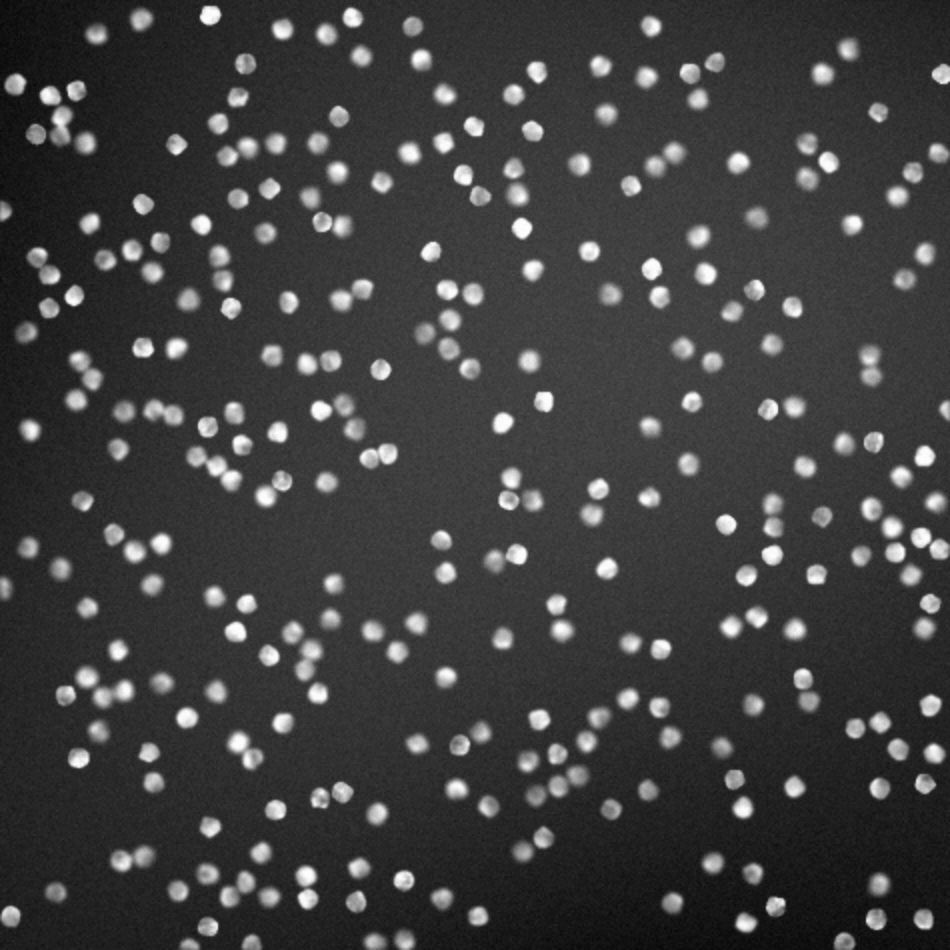
\includegraphics[width=80mm]{../images/BBBC4-1.jpg}
\subcaption{2Gray1.tif (image)}
\label{fig:BBBC004_img}
\end{minipage}
\hfill
\begin{minipage}[c]{0.4\linewidth}
\centering
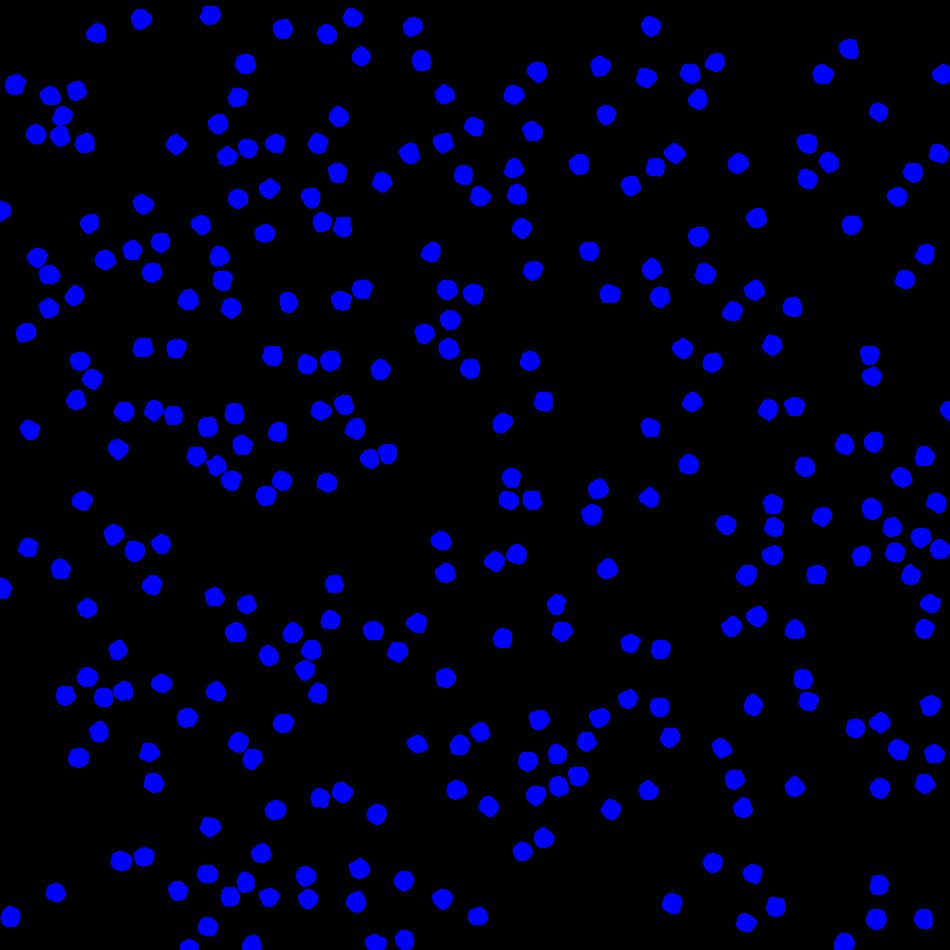
\includegraphics[width=80mm]{../images/BBBC4-1-F.jpg}
\subcaption{1.tif (mask)}
\label{fig:BBBC004_F}
\end{minipage}
\caption{Sample data from the BBBC4 Database with mask as ground truth}
\end{figure}

\subsection{Outlines of individual objects}
In this case, a human outlines each cell in the image in order to indicate which pixels belong to which cell. The ground truth is provided as binary images, with black outlines on a white background.

\begin{figure}[H]
\begin{minipage}[c]{0.4\linewidth}
\centering
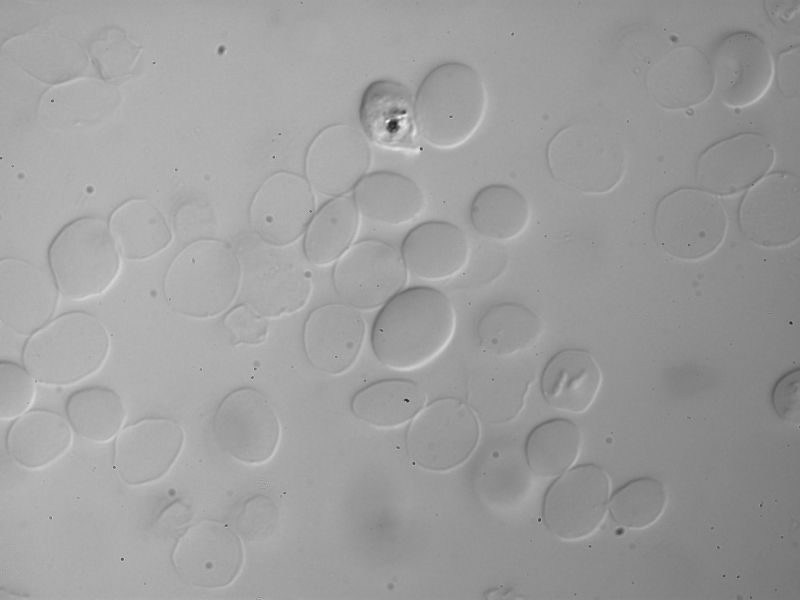
\includegraphics[width=80mm]{../images/48hr-001-DIC.jpg}
\subcaption{48hr-001-DIC.jpg (image)}
\label{fig:BBBC009_img}
\end{minipage}
\hfill
\begin{minipage}[c]{0.4\linewidth}
\centering
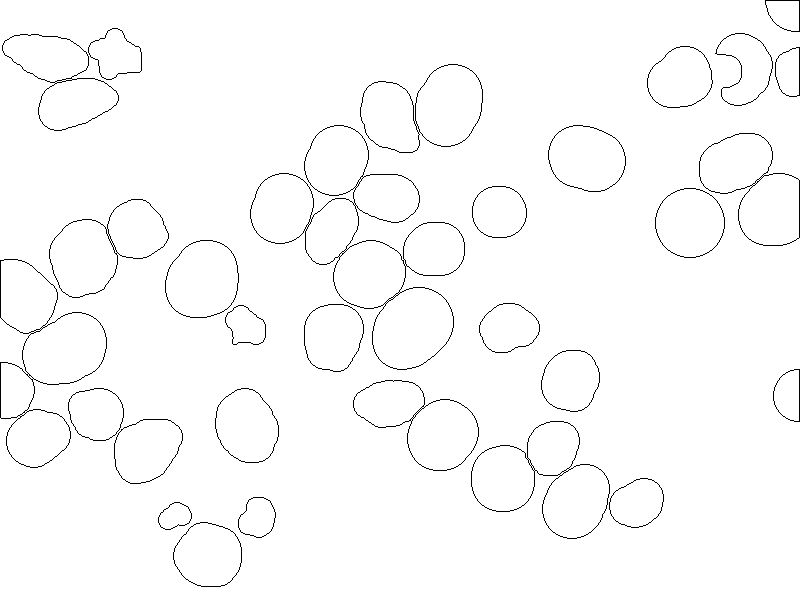
\includegraphics[width=80mm]{../images/48hr-001-DIC_.jpg}
\subcaption{48hr-001-DIC.jpg (edge mask)}
\label{fig:BBBC009_O}
\end{minipage}
\caption{Sample data from the BBBC9 Database with edge mask (outlines) as ground truth}
\end{figure}

\subsection{Biological labels}
In these cases, the experiments have been prepared with control samples for which we know the expected biological result. The types of controls that are available dictate the type of statistic that can be calculated.

\subsection{Location}
In this case, the ground truth consists of the X, Y, and optionally Z location of objects (typically their centroids similar to ALL-IDB1 Annotation \ref{fig:Im006.xyc.jpg}) .

\subsection{Bounding Boxes}
Bounding boxes are rectangles completely enclosing an object.

\newpage

\section{WBC Image Dataset : Fast and Robust Segmentation of White Blood Cell Images by Self-supervised Learning}
This is two datasets of white blood cell (WBC) images used for “Fast and Robust Segmentation of White Blood Cell Images by Self-supervised Learning”, which can be used to evaluate cell image segmentation methods \textsuperscript{\cite{Zheng2018}}.
This collection contains two datasets different from each other in terms of the image color, cell shape, background, etc. The ground truth segmentation results are manually sketched by domain experts, where the nuclei, cytoplasms and background including red blood cells are marked in white, gray and black respectively. 

\subsection{Dataset 1}
was obtained from Jiangxi Tecom Science Corporation \textsuperscript{\cite{2022_tecom-cn}}, China. It contains three hundred 120×120 images of WBCs and their color depth is 24 bits. The images were taken by a Motic Moticam Pro 252A optical microscope camera with a N800-D motorized auto-focus microscope.

\begin{figure}[H]
\centering
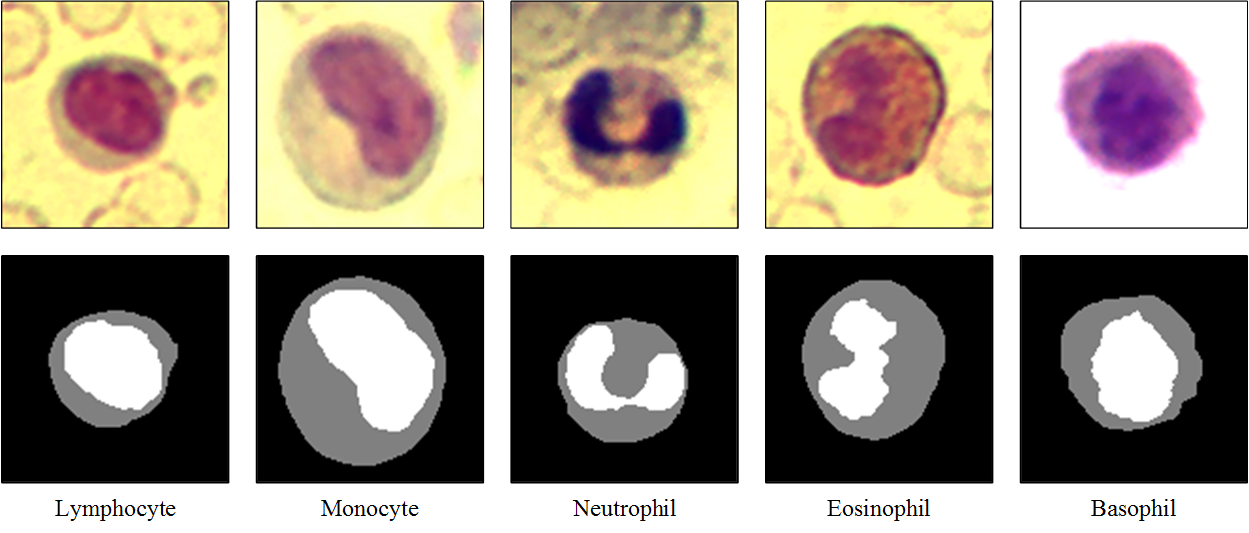
\includegraphics[width=\linewidth]{../images/WBC_Dataset1.png}
\caption{Sample data from WBC\_Segmentaion Dataset 1}
\label{fig:WBC_Dataset1_sample}
\end{figure}

\subsection{Dataset 2}
consists of one hundred 300×300 color images, which were collected from the CellaVision blog \textsuperscript{\cite{2022_cellavision}}. The cell images are generally purple and may contain many red blood cells around the white blood cells.

\begin{figure}[H]
\centering
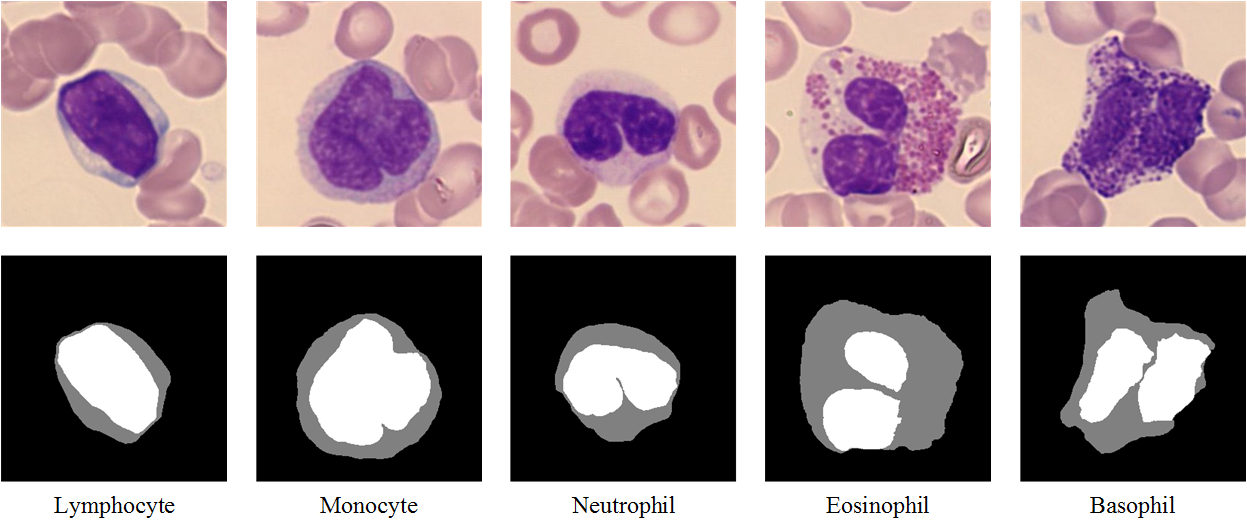
\includegraphics[width=\linewidth]{../images/WBC_Dataset2.png}
\caption{Sample data from WBC\_Segmentaion Dataset 2}
\label{fig:WBC_Dataset2_sample}
\end{figure}


\subsection{Annotation}
The class labels of each image in Dataset 1 and Dataset 2 are stored in csv files. The labels (1- 5) represent neutrophil, lymphocyte, monocyte, eosinophil and basophil, respectively.


\subsection{A large dataset of white blood cells containing cell locations and types, along with segmented nuclei and cytoplasm}

The database is provided by \href{https://raabindata.com/free-data/#double-labeled-cropped-cells}{RabinData} and \textsuperscript{\cite{Kouzehkanan2022}} which devides on two separate datasets:
\subsubsection{Raabin-WBC Data}
Contains 4 sub-Datasets:
\begin{itemize}
    \item \textbf{Double-labeled cropped cells} : Double-labeled cropped cells are also provided containing only five main classes including mature neutrophils, lymphocytes (small and large), eosinophils, monocytes, and basophils. 
    \item \textbf{Nucleus\_cytoplasm\_Ground truths} : in this sub-Dataset they prepared the ground truths of the cytoplasm and the nucleus for a proper number of cropped white blood cells. For this purpose, 1145 cropped images including 242 lymphocytes, 242 monocytes, 242 neutrophils, 201 eosinophils, and 218 basophils were randomly selected, and their ground truths were extracted by an expert.
    \item \textbf{Microscopic images were taken by the Olympus CX18 microscope and the Samsung Galaxy S5 camera and the 4th database with contain images taken by Zeiss microscope and the LG G3 camera } : in these two sub-Datasets. Corresponding to each microscopic image, a dictionary (.json format) file containing the following information about that image was provided:
    \begin{itemize}
        \item Information about the blood elements in the image including their coordinates and labels.
        \item Information about the blood smears including staining method and the type of the disease.
        \item Information about the microscope includes the type of microscope and its magnification size.
        \item The type of camera used.
    \end{itemize}
\end{itemize}

\subsubsection{Raabin-Leukemia Data}
Contains 4 sub-Datasets:
\begin{itemize}
    \item \textbf{Acute Lymphoblastic Leukemia}  
    \item \textbf{Acute Myeloblastic Leukemia} 
    \item \textbf{Chronic Lymphocytic Leukemia}
    \item \textbf{Chronic Myelogenous Leukemia}
\end{itemize}
In each of these sub-Dataset, All samples were taken from patients who had referred to our collaborator medical laboratory (Takht-e Tavous Laboratory in Tehran, Iran). It should be notices Zeiss microscope and LG J3 smartphone camera had been used for imaging.
\subsection{BCCD}
BCCD Dataset is a small-scale dataset for blood cells detection. The original data and annotations are from \href{https://github.com/cosmicad/dataset}{cosmicad}  and \href{https://github.com/akshaylamba/all_CELL_data}{akshaylamba}. \\
In this project, the Faster R-CNN algorithm from keras-frcnn for Object Detection is used. From this dataset, nicolaschen1 developed two Python scripts to make preparation data (CSV file and images) for recognition of abnormalities in blood cells on medical images.

\begin{figure}[H]
\centering
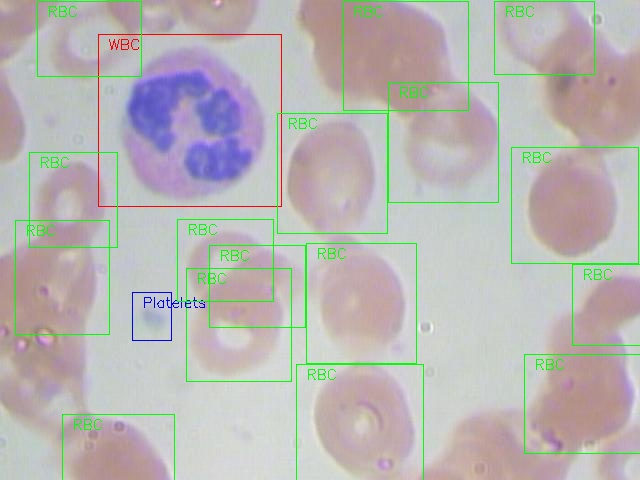
\includegraphics[width=\linewidth]{../images/BBCD1.jpg}
\caption{Sample data from BBCD}
\label{fig:BBCD1}
\end{figure}

In this database they use bounding boxes to locate the cells and each bounding box has the type of cell RBC or WBC and platlets. they are using the VOC format as a database architecture.

\newpage
\section{Conclusion}
\hspace*{0.16in}



\newpage


\newpage

\section{Introduction}
\vspace{0.2in}
\hspace*{0.16in}

\section{Artificial Intelligence}
\subsection{Definition}

\subsection{Machine Learning}

\begin{itemize}
  \item \textbf{Linear Regression:}
  \item \textbf{Support Vector Machines:}
  \item \textbf{Gradient Descent:}
\end{itemize}

\subsection{Deep Learning}
\subsubsection{Neural Networks}
Artificial neural networks (ANNs) are comprised of a node layers, containing an input layer, one or more hidden layers, and an output layer. Each node, or artificial neuron, connects to another and has an associated weight and threshold. If the output of any individual node is above the specified threshold value, that node is activated, sending data to the next layer of the network. Otherwise, no data is passed along to the next layer of the network.


\begin{figure}[H]
\centering
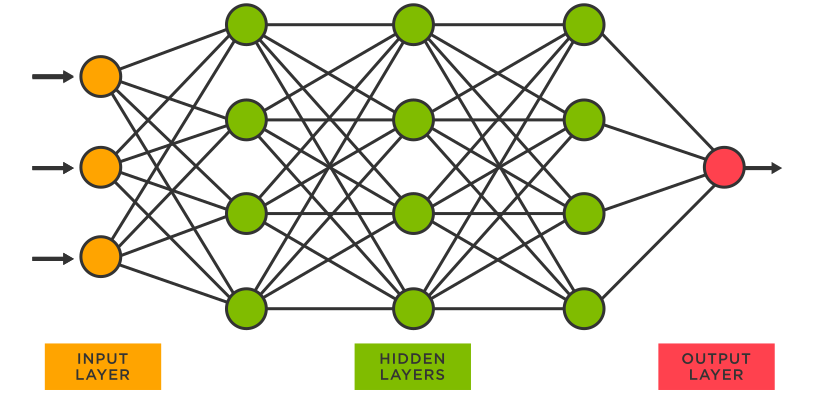
\includegraphics[width=\linewidth]{../images/neural-network-diagram.png}
\caption{Architecture of Neural Network}
\label{fig:NN}
\end{figure}

Neural networks rely on training data to learn and improve their accuracy over time. However, once these learning algorithms are fine-tuned for accuracy, they are powerful tools in computer science and artificial intelligence, allowing us to classify and cluster data at a high velocity. Tasks in speech recognition or image recognition can take minutes versus hours when compared to the manual identification by human experts. One of the most well-known neural networks is Google’s search algorithm.

if we dive into the details, we can consider that each node has it's linear regression model, composed of input data, weights, a bias (or threshold), and an output. The formula would look something like equation \ref{eq:NN-Node-Activation}:

%\begin{figure}[H]
%\centering
%
\includegraphics[width=\linewidth]{../images/NN-Node-equation.png}
%\caption{Architecture of Neural Network}
%\label{fig:NN}
%\end{figure}

\begin{equation}
    \sum_{i=1}^{m} W_{i}X_{i} + bias = W_{1}X_{1} + W_{2}X_{2} + W_{3}X_{3} + bias
    \label{eq:NN-Node-Activation}
\end{equation}

\begin{equation}
    output = f(x) = 
    \begin{cases}
        1 & if \sum_{i=1}^{m} W_{1}X_{1} + b \leq 0 \\
        0 & if \sum_{i=1}^{m} W_{1}X_{1} + b < 0
    \end{cases}
    \label{eq:NN-Node-Activation2}
\end{equation}

Once an input layer is determined, weights are assigned. These weights help determine the importance of any given variable, with larger ones contributing more significantly to the output compared to other inputs. All inputs are then multiplied by their respective weights and then summed (similar to eaquation \ref{eq:NN-Node-Activation}). Afterward, the output is passed through an activation function as we can see in equation \ref{eq:NN-Node-Activation2}, which determines the output. If that output exceeds a given threshold, it “fires” (or activates) the node, passing data to the next layer in the network. This results in the output of one node becoming in the input of the next node. This process of passing data from one layer to the next layer defines this neural network as a feedforward network.




\subsubsection{Convolutional Neural Networks}
CNNs or ConvNets are among the most successful and widely used architectures in the deep learning community, especially for computer vision tasks . CNNs were initially proposed by Fukushima in his seminal paper on the “Neocognitron” \textsuperscript{\cite{fukushima_Neocognitron}}.

\begin{figure}[H]
\centering
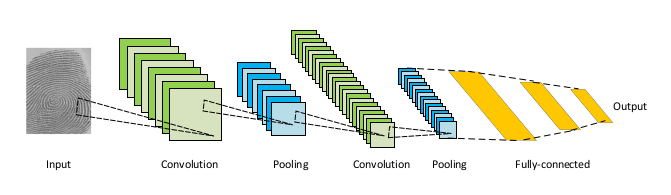
\includegraphics[width=\linewidth]{../images/CNN.png}
\caption{Architecture of convolutional neural networks. From \textsuperscript{\cite{minaee2021image}}}
\label{fig:CNN}
\end{figure}

Convolutional neural networks are distinguished from other neural networks by their superior performance with image, speech, or audio signal inputs. They have three main types of layers, which are:

\begin{itemize}
    \item Convolutional layer
    \item Pooling layer
    \item Fully-connected (FC) layer
\end{itemize}

The convolutional layer is the first layer of a convolutional network. While convolutional layers can chained by additional convolutional layers or pooling layers, the fully-connected layer is the final layer. With each layer, the CNN increases in its complexity, identifying greater portions of the image. Earlier layers focus on simple features, such as colors and edges. As the image data progresses through the layers of the CNN, it starts to recognize larger elements or shapes of the object until it finally identifies the intended object. 
    
    
\begin{enumerate}
    \item \textbf{Convolutional layer} : \\
        The convolutional layer is the core building block of a CNN, and it is where the majority of computation occurs. It requires a few components, which are input data, a filter, and will output a feature map. Let’s assume that the input will be a color image, which is made up of a matrix of pixels in 3D. This means that the input will have three dimensions—a height, width, and depth—which correspond to RGB in an image. We also have a feature detector, also known as a kernel or a filter, which will move across the receptive fields of the image, checking if the feature is present. This process is known as a convolution. \textsuperscript{\cite{CNN-IBM}} \\
        The feature detector is a two-dimensional (2-D) array of weights, which represents part of the image. While they can vary in size, the filter size is typically a 3x3 matrix; this also determines the size of the receptive field. The filter is then applied to an area of the image, and a dot product is calculated between the input pixels and the filter. This dot product is then fed into an output array. Afterwards, the filter shifts by a stride, repeating the process until the kernel has swept across the entire image. The final output from the series of dot products from the input and the filter is known as a feature map, activation map, or a convolved feature.
        \begin{figure}[H]
            \centering
            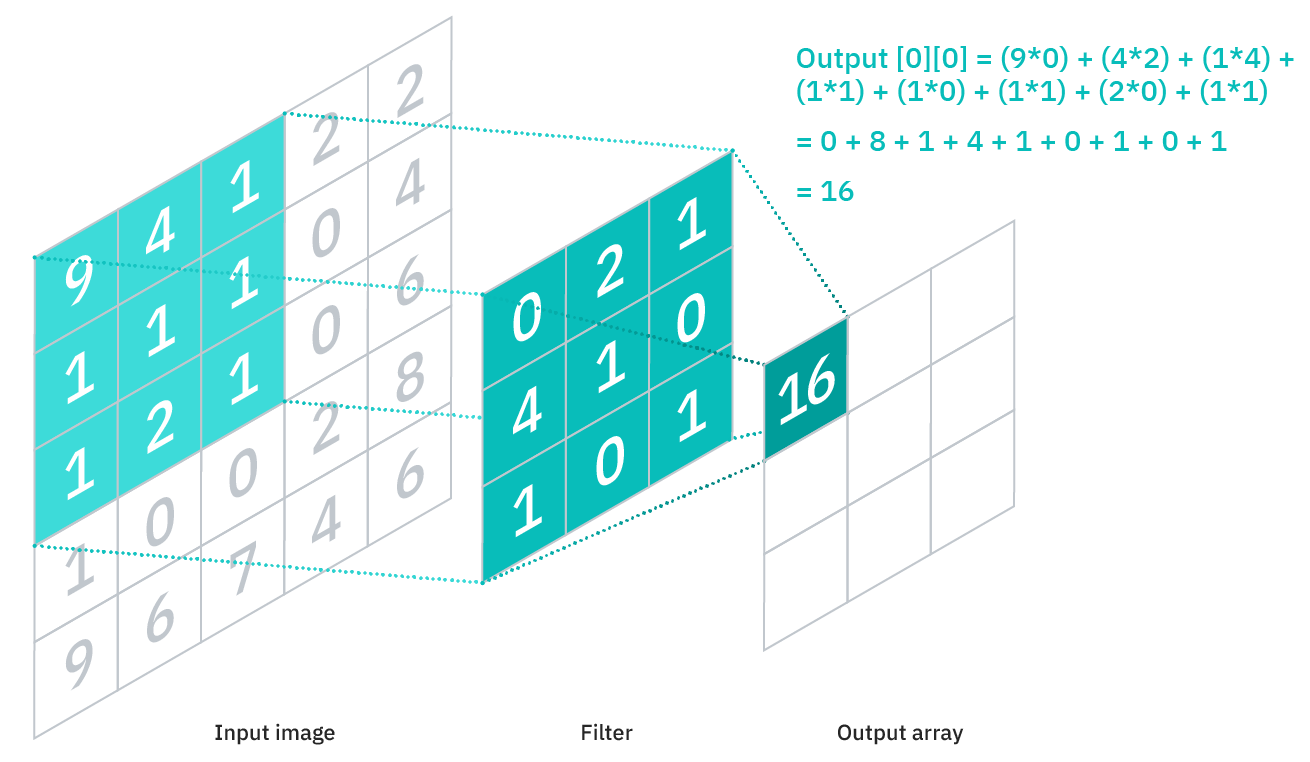
\includegraphics[width=10cm]{../images/CNN-kernel.png}
            \caption{CNN kernel}
            \label{fig:CNN-kernel}
        \end{figure}
        as we can see in the fig \ref{fig:CNN-kernel}, the kernel will browse all the matrix by shifting it's position. where the weights in the kernel will remain fixed as it moves across the image, which is also known as parameter sharing. Some parameters, like the weight values, adjust during training through the process of backpropagation and gradient descent. However, there are three hyperparameters which affect the volume size of the output that need to be set before the training of the neural network begins. These include:
        \begin{itemize}
            \item \textbf{The number of filters} affects the depth of the output. For example, three distinct filters will give us three different feature maps, creating a depth of three.
            \item \textbf{Stride} is the distance, or number of pixels, that the kernel moves over the input matrix. While stride values of two or greater is rare, a larger stride yields a smaller output.
            \item \textbf{Zero-padding }is usually used when the filters do not fit the input image. This sets all elements that fall outside of the input matrix to zero, producing a larger or equally sized output. There are three types of padding:
            \begin{itemize}
                \item \textbf{Valid padding}: This is also known as no padding. In this case, the last convolution is dropped if dimensions do not align.
                \item \textbf{Same padding}: This padding ensures that the output layer has the same size as the input layer
                \item \textbf{Full padding}: This type of padding increases the size of the output by adding zeros to the border of the input.
            \end{itemize}
        \end{itemize}
        
        \begin{figure}[H]
            \centering
            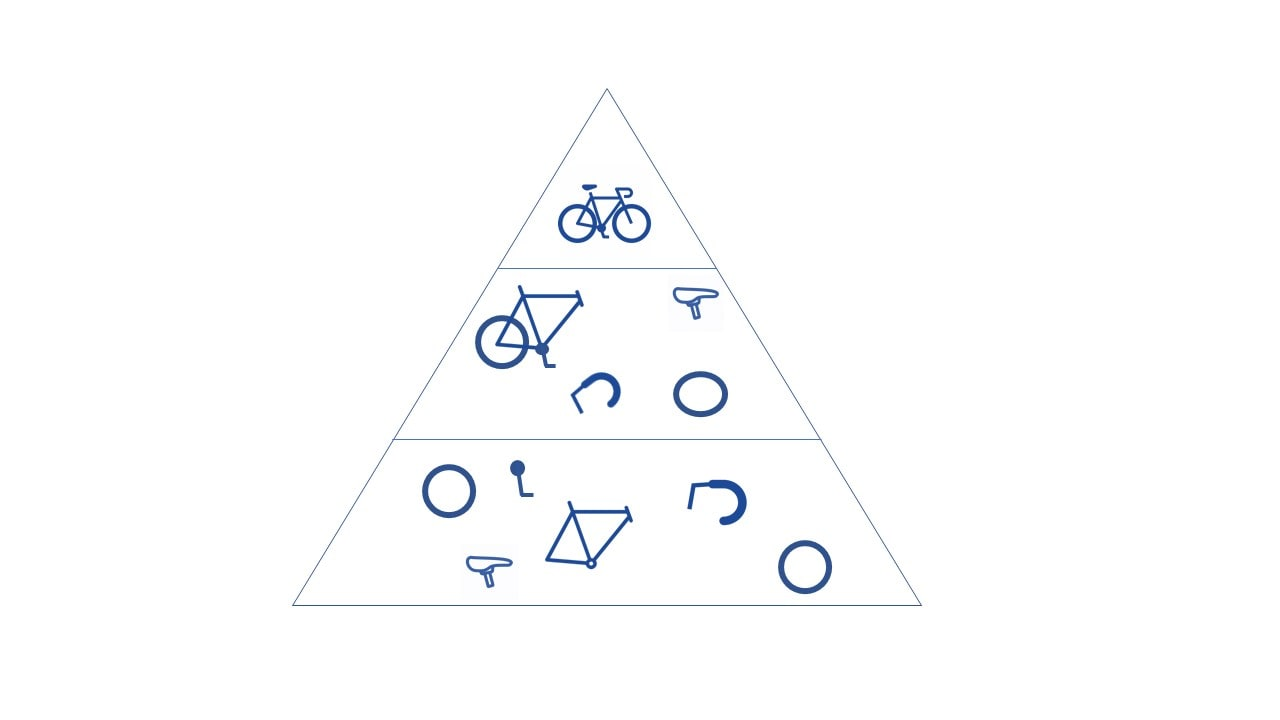
\includegraphics[width=10cm]{../images/CNN-Feature-Hierarchy.jpg}
            \caption{Feature Hierarchy}
            \label{fig:CNN-Feature-Hierarchy}
        \end{figure}
        
        After each convolution operation, a CNN applies an activation function to the feature map, the most used activation function is the Rectified Linear Unit (ReLU).\\
        As we mentioned earlier, when we chain convolutional layers, the structure of the CNN can become hierarchical as the later layers can see the pixels within the receptive fields of prior layers.  As an example, let’s assume that we’re trying to determine if an image contains a bicycle. You can think of the bicycle as a sum of parts. It is comprised of a frame, handlebars, wheels, pedals, et cetera. Each individual part of the bicycle makes up a lower-level pattern in the neural net, and the combination of its parts represents a higher-level pattern, creating a feature hierarchy within the CNN.
    \item \textbf{Pooling Layer}:\\
        Pooling layers, also known as downsampling, conducts dimensionality reduction, reducing the number of parameters in the input. Similar to the convolutional layer, the pooling operation sweeps a filter across the entire input, but the difference is that this filter does not have any weights. Instead, the kernel applies an aggregation function to the values within the receptive field, populating the output array. There are two main types of pooling:
        \begin{itemize}
            \item \textbf{Max pooling}: As the filter moves across the input, it selects the pixel with the maximum value to send to the output array. As an aside, this approach tends to be used more often compared to average pooling.
            \item \textbf{Average pooling}: As the filter moves across the input, it calculates the average value within the receptive field to send to the output array.
        \end{itemize}
        
        While a lot of information is lost in the pooling layer, it also has a number of benefits to the CNN. They help to reduce complexity, improve efficiency, and limit risk of overfitting.
    
    \item \textbf{Fully-Connected Layer}:\\
        The name of the fully-connected layer aptly describes itself. The pixel values of the input image are not directly connected to the output layer in partially connected layers. However, in the fully-connected layer, each node in the output layer connects directly to a node in the previous layer.

        This layer performs the task of classification based on the features extracted through the previous layers and their different filters. While convolutional and pooling layers tend to use ReLu functions or other activation functions, FC layers usually leverage a softmax or sigmoid activation function to classify inputs appropriately, producing a probability from 0 to 1.
        
\end{enumerate}



\section{CNN architectures}
\vspace{0.2in}
\hspace*{0.16in}

\subsection{U-Net}

\subsection{SegNet}

\subsection{VGG}

\section{Image Processing Methods}
\vspace{0.2in}
\hspace*{0.16in}


\newpage

\section{Introduction}
\vspace{0.2in}
\hspace*{0.16in}
As part of our research, we have treated the case of segmenting and counting Red, White blood cells and platelets which also known as CBC (Complete Blood Count), we are using the ALL-IDB\textsuperscript{\cite{pm77-2n23-20}} Dataset to train and evaluate our models.
In our case study, and from multiple articles, we can see that U-Net and Segnet models are dominating the field of cell segmentation and Medical Computer vision in general.
In this chapter, we test out both U-Net and Segnet models, and analyse the results by comparing results of the two architectures.
We will also explore different machine learning algorithms for both preprocessing and postprocessing.

\section{Our approach}
\vspace{0.2in}
\hspace*{0.16in}
From all of the intel we have gathered, and previously read articles, all of cell segmentation (blood cell segmentation in particular) are mostly using U-Net and Segnet archtectures for segmenting blood cell images.
We have implemented both the U-Net and Segnet models.
In the following sections, we will briefly analyze and compare both convolutional neural network (CNN) models with their perspective results.
And explain all the postprocessing methods we used for the counting of blood cells (red, white and platelets)

\section{U-Net}
\subsection{Definition}
The U-Net is a convolutional neural network that was developed for biomedical image segmentation at the Computer Science Department of the University of Freiburg. The network is based on the fully convolutional network and its architecture was modified and extended to work with fewer training images and to yield more precise segmentations. In our case we are using DO-UNet from \textsuperscript{\cite{10.1007/978-3-030-44584-3_31}} which is a modified U-Net to produce dual outputs, which also known as contour aware network was first demonstrated by the DCAN architecture \textsuperscript{\cite{chen2016dcan}}.  Based on a simple FCN, DCAN was trained to use the outer
contours of the areas of interest to guide the training of the segmentation masks. This led to improved semantic and instance segmentation of the model, which in their case, looked at non-overlapping features in biomedical imaging.
With the aim of counting closely co-located and overlapping cells, we are predominantly interested in the correct detection of individual objects as
opposed to the exact precision of the segmentation mask itself. An examination
of the hidden convolutional layers of the classical U-Net showed that the penultimate layer of the network extracts information about the edges of the cells, so the idea is to output the cell mask + edge mask then do a substraction to break the overlapping cells.

\subsection{Architecture}
They Started with the classical U-Net then reduced the number of
convolutional layers and skip connections in the model. Simultaneously, they minimised the complexity of the model by looking at smaller input regions of the images, thus minimising the memory footprint of the model. They follow the approach of Ronneberger et. al. \textsuperscript{\cite{10.1007/978-3-030-44584-3_31}} by using unpadded convolutions throughout the network, resulting in a model with smaller output edge and mask (100 × 100 px) corresponding to a central region of a larger (188 × 188 px) input image region. DO-U-Net uses two, independently trained, output layers of identical size. Figure \ref{fig:DO-UNET} shows the DO-U-Net architecture.

\begin{figure}[H]
\centering
  \vspace{-0.1in}
    \centerline{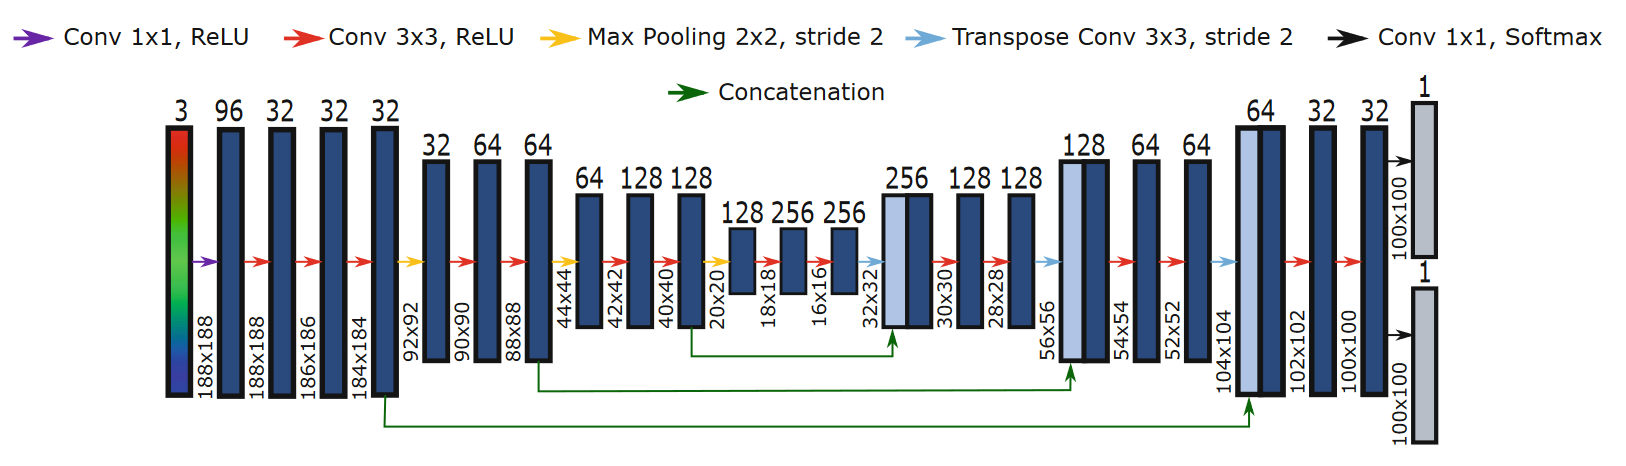
\includegraphics[width = \linewidth]{../images/DO-UNET.png}}
    \caption{DO-UNet architecture}
    \label{fig:DO-UNET}
\end{figure}

\section{Segnet}
\subsection{Definition}
The SegNet neural network, developed by Alex Kendall, Vijay Badrinarayanan, and Roberto Cipolla, all from the University of Cambridge, is a convolutional neural network used for semantic pixel wise labeling. This problem is more commonly called semantic segmentation. \textsuperscript{\cite{badrinarayanan2017segnet}}

\subsection{Architecture}
SegNet has an encoder network and a corresponding decoder network, followed by a final pixelwise classification layer. This architecture is illustrated in the below figure.
With 13 encoder layers obtained from the VGG16 network, and 13 decoder layers to match the same number of encoder layers. The final decoder output is fed to a multi-class soft-max classifier to produce class probabilities for each pixel independently (pixelwise).

Each encoder in the encoder network performs convolution with a filter bank to produce a set of feature maps. These are then batch normalized. Then an element-wise rectified- linear non-linearity (ReLU) max(0, x) is applied. Following that, max-pooling with a 2x2 window and stride 2 (non-overlapping window) is performed and the resulting output is sub-sampled by a factor of 2. Max-pooling is used to achieve translation invariance over small spatial shifts in the input image.

The appropriate decoder in the decoder network upsamples its input feature map(s) using the memorized max-pooling indices from the corresponding encoder feature map(s). This step pro- duces sparse feature map(s). This SegNet decoding technique is illustrated in the below figure.
These feature maps are then convolved with a trainable decoder filter bank to produce dense feature maps. A batch normalization step is then applied to each of these maps. Note that the decoder corresponding to the first encoder (closest to the input image) produces a multi-channel feature map, although its encoder input has 3 channels (RGB).
This is unlike the other decoders in the network which produces feature maps with the same number of size and channels as their encoder inputs. The high dimensional feature representation at the output of the final decoder is fed to a trainable soft-max classifier.
This soft-max classifies each pixel independently. The output of the soft-max classifier is a K channel image of probabilities where K is the number of classes. The predicted segmentation corresponds to the class with maximum probability at each pixel. \textsuperscript{\cite{badrinarayanan2017segnet}}

\vspace{0.2in}

\begin{figure}[H]
\centering
  \vspace{-0.1in}
    \centerline{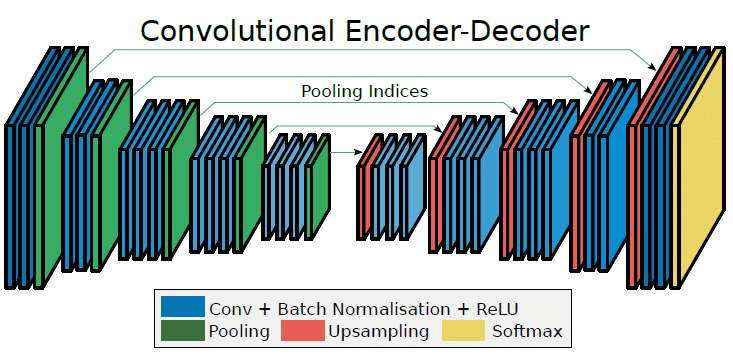
\includegraphics[width = 4in, height = 2.2in]{../images/segnet.png}}
    \caption{SegNet architecture}
\end{figure}

\subsection{Dataset}
For the segnet model, we have decided to test th ALL-IDB1 dataset, which contains 108 blood cell images, of which 10 images with their perspective masks and edge masks were chosen for red blood cell training and 3 as a test dataset, for white blood cells 73 images with their masks, and 33 as a test dataset.
For platelets, we used 71 for training and 31 as a test dataset.
Only red blood cells have edge masks, because we need to get rid of overlapped cells, white blood cells and platelets dont need the edge masks, using masks only can retrieve all the necessary features, because both white blood cells and platelets rarely overlap.
The images will be sliced and rescaled to 128x128 to match the input shape of the Segnet model.
The resulting train dataset will be 3916 image, mask, and edge tiles (a total of 11748 tiles).
For the test dataset 1072 image, mask, and edge tiles (a total of 3216 tiles) for red blood cells.
As for white blood cells, 28126 image and mask tiles were used for training (a total of 56252 tiles), and 15892 image and mask tiles were used as a test dataset for white blood cells (a total of 31784 tiles).
Finally, for platelets we used 27650 image and mask tiles were used for training (a total of 55300), and 14410 image and mask tiles as a test dataset for platelets (a total of 28820).

\vspace{0.1in}

% Please add the following required packages to your document preamble:
% \usepackage{multirow}
% \usepackage{graphicx}
% \usepackage[table,xcdraw]{xcolor}
% If you use beamer only pass "xcolor=table" option, i.e. \documentclass[xcolor=table]{beamer}
\begin{table}[H]
\centering
\resizebox{\textwidth}{!}{%
\begin{tabular}{|cc|c|c|c|c|c|c|}
\hline
\multicolumn{2}{|c|}{{\color[HTML]{000000} \textbf{Dataset}}}                                                                     & {\color[HTML]{000000} \textbf{\begin{tabular}[c]{@{}c@{}}Train\\ images\end{tabular}}} & {\color[HTML]{000000} \textbf{\begin{tabular}[c]{@{}c@{}}Test\\ images\end{tabular}}} & {\color[HTML]{000000} \textbf{\begin{tabular}[c]{@{}c@{}}Train\\ Tiles\end{tabular}}} & {\color[HTML]{000000} \textbf{\begin{tabular}[c]{@{}c@{}}Test\\ Tiles\end{tabular}}} & {\color[HTML]{000000} \textbf{\begin{tabular}[c]{@{}c@{}}Total\\ images\end{tabular}}} & {\color[HTML]{000000} \textbf{\begin{tabular}[c]{@{}c@{}}Total\\ tiles\end{tabular}}} \\ \hline
\multicolumn{1}{|c|}{{\color[HTML]{000000} }}                                             & {\color[HTML]{000000} \textbf{Image}} & {\color[HTML]{000000} 10}                                                              & {\color[HTML]{000000} 3}                                                              & {\color[HTML]{000000} 3916}                                                           & {\color[HTML]{000000} 1072}                                                          & {\color[HTML]{000000} 13}                                                              & {\color[HTML]{000000} \textbf{4988}}                                                  \\ \cline{2-8} 
\multicolumn{1}{|c|}{{\color[HTML]{000000} }}                                             & {\color[HTML]{000000} \textbf{Mask}}  & {\color[HTML]{000000} 10}                                                              & {\color[HTML]{000000} 3}                                                              & {\color[HTML]{000000} 3916}                                                           & {\color[HTML]{000000} 1072}                                                          & {\color[HTML]{000000} 13}                                                              & {\color[HTML]{000000} \textbf{4988}}                                                  \\ \cline{2-8} 
\multicolumn{1}{|c|}{\multirow{-3}{*}{{\color[HTML]{000000} \textbf{Red Blood Cells}}}}   & {\color[HTML]{000000} \textbf{Edge}}  & {\color[HTML]{000000} 10}                                                              & {\color[HTML]{000000} 3}                                                              & {\color[HTML]{000000} 3916}                                                           & {\color[HTML]{000000} 1072}                                                          & {\color[HTML]{000000} 13}                                                              & {\color[HTML]{000000} \textbf{4988}}                                                  \\ \hline
\multicolumn{1}{|c|}{{\color[HTML]{000000} }}                                             & {\color[HTML]{000000} \textbf{Image}} & {\color[HTML]{000000} 73}                                                              & {\color[HTML]{000000} 33}                                                             & {\color[HTML]{000000} 28126}                                                          & {\color[HTML]{000000} 15892}                                                         & {\color[HTML]{000000} 106}                                                             & {\color[HTML]{000000} \textbf{44018}}                                                 \\ \cline{2-8} 
\multicolumn{1}{|c|}{\multirow{-2}{*}{{\color[HTML]{000000} \textbf{White Blood Cells}}}} & {\color[HTML]{000000} \textbf{Mask}}  & {\color[HTML]{000000} 73}                                                              & {\color[HTML]{000000} 33}                                                             & {\color[HTML]{000000} 28126}                                                          & {\color[HTML]{000000} 15892}                                                         & {\color[HTML]{000000} 106}                                                             & {\color[HTML]{000000} \textbf{44018}}                                                 \\ \hline
\multicolumn{1}{|c|}{{\color[HTML]{000000} }}                                             & {\color[HTML]{000000} \textbf{Image}} & {\color[HTML]{000000} 71}                                                              & {\color[HTML]{000000} 31}                                                             & {\color[HTML]{000000} 27650}                                                          & {\color[HTML]{000000} 14410}                                                         & {\color[HTML]{000000} 102}                                                             & {\color[HTML]{000000} \textbf{42060}}                                                 \\ \cline{2-8} 
\multicolumn{1}{|c|}{\multirow{-2}{*}{{\color[HTML]{000000} \textbf{Platelets}}}}         & {\color[HTML]{000000} \textbf{Mask}}  & {\color[HTML]{000000} 71}                                                              & {\color[HTML]{000000} 31}                                                             & {\color[HTML]{000000} 27650}                                                          & {\color[HTML]{000000} 14410}                                                         & {\color[HTML]{000000} 102}                                                             & {\color[HTML]{000000} \textbf{42060}}                                                 \\ \hline
\end{tabular}%
}
\caption{Dataset used for segnet}
\label{Dataset used for segnet}
\end{table}


\subsection{Dataset augmentation}
We used the same dataset augmention on all cells (red, white blood cells, and platelets).
The augmentation we used was custom which involves the following steps:
\begin{enumerate}
    \item Pick a random image from the train dataset.
    \item Get the x and y coordinates randomly from the chosen image.
    \item Rescale the image randomly.
    \item Find the edges of a box around the image chip and the mask chip.
    \item Take a slice of the image and mask accordingly.
    \item Skip empty image chips (masks, and edge chips for red blood cells).
    \item Resize the image and mask chip to 128x128.
    \item Randomly rotate and flip the image chip.
    \item Randomly augment the colors (luminosity and saturation).
    \item Rescale the chip back to normal.
\end{enumerate}

\section{Counting}
\vspace{0.2in}
\hspace*{0.16in}
After having segmented blood cell images (red, white blood cells and platelets), we use many postprocessing methods (machine learning algorithms) to get the coordinates of circles and count them.
Here are all the algorithms we used to get an relatively accurate blood cell count:

\subsection{Circle Hough Transform}
Circle Hough Transform (CHT) is machine learning algorithm used to extract features (circles) from imperfect images.
We modified its parameters (Minimum distribution, Minimum and Maximum radius...) for each type of blood cells (red, white and platelets).\\
Note that we do not rely on this approach to count white blood cells, because most white blood cells have different shapes.
Therefore, this method is useless when it comes to white blood cells counting.

\subsection{Connected Component Labeling}
Connected Component Labeling (CCL) is machine learning algorithm used to detect connected regions in a binary image.
Before applying the connected component labeling, we convert the images to grayscale. Then, a binary threshold is applied to the images to get binary values.
Finally, we apply the connected component labeling to get the labels and map component labels to the resulting image.

\subsection{Watershed}
Watershed algorithms (also called drainage divide) are used in image processing primarily for object segmentation purposes, that is, for separating different objects in an image. the main purpose of using watershed in this phase is to segment the touching and overlapping cells, the watershed takes two inputs, first i takes an image with different intensity levels in our-case the distance transform of our mask where the intensity levels represents reliefs. the second input is the water sources in our-case we extracted local maxima from the distance transform image. we can see below the steps we used to count the cells.

\begin{enumerate}
    \item \textbf{Compute the Euclidean distance}: we compute euclidean distance from every binary pixel to the nearest zero pixel, this map will be used as our relief map in the watershed algorithm.
    \item \textbf{We find peaks in the distance map}: we search for peaks in our euclidean distance map which is the local maxima in each region, which are the highest points in the map (higher intensity levels), which we will use as water sources in the watershed algorithm.
    \item \textbf{apply connected component labeling on the peak map}: we apply CCL algorithm which is also called 8-connectivity algorithm to label the peaks (label each water source).
    \item \textbf{apply the Watershed algorithm on the reversed distance map using the labeled peaks}: at the end we feed the reversed distance map and the water sources map (local maxima) to the watershed algorithm to get the segmented image. 
\end{enumerate}

\section{Metrics And Loss Functions}
Loss functions are one of the important ingredients in deep learning-based medical image segmentation methods. In the past four years, more than 20 loss functions have been proposed for various segmentation tasks. Most of them can be used in any segmentation tasks in a plug-and-play way, we can see in (fig \ref{fig:LossFunctions}) the relations between the most used  Loss Functions, we will present below the used Loss Functions in our paper.

\begin{figure}[H]
\centering
  \vspace{-0.1in}
    \centerline{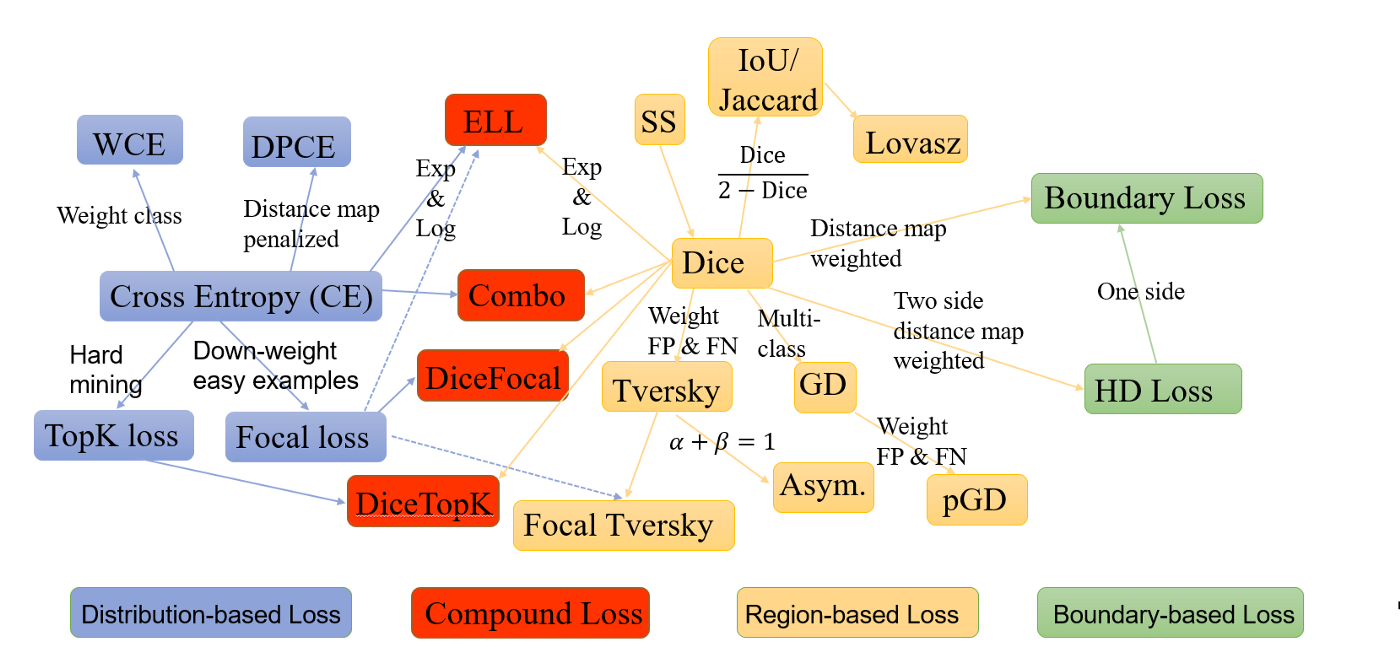
\includegraphics[width = \linewidth]{../images/LossFunctions.png}}
    \caption{Loss Functions}
    \label{fig:LossFunctions}
\end{figure}

In this section, we will discuss the loss functions and metrics that we used to train and evaluate our models.

When performing classification predictions (pixel-wise classification in our case) there's four types of outcomes that could occur.

\begin{enumerate}
    \item \textbf{True positives} are when you predict an observation belongs to a class and it actually does belong to that class.
    \item \textbf{True negatives} are when you predict an observation does not belong to a class and it actually does not belong to that class.
    \item \textbf{False positives} occur when you predict an observation belongs to a class when in reality it does not.
    \item \textbf{False negatives} occur when you predict an observation does not belong to a class when in fact it does.
\end{enumerate}

These four outcomes are often plotted on a confusion matrix. The following confusion matrix is an example for the case of binary classification. This matrix should be generated making predictions on the test data and then identifying each prediction as one of the four possible outcomes described above.

\vspace{0.1in}

\begin{table}[H]
\centering
\begin{tabular}{cc|cc|}
\cline{3-4}
\multicolumn{2}{c|}{\multirow{2}{*}{}}                                                                                        & \multicolumn{2}{c|}{\textbf{Actual Values}}             \\ \cline{3-4} 
\multicolumn{2}{c|}{}                                                                                                         & \multicolumn{1}{c|}{\textbf{Yes (1)}} & \textbf{No (0)} \\ \hline
\multicolumn{1}{|c|}{\multirow{2}{*}{\textbf{\begin{tabular}[c]{@{}c@{}}Predicted\\ Values\end{tabular}}}} & \textbf{Yes (1)} & \multicolumn{1}{c|}{\textbf{TP}}      & \textbf{FP}     \\ \cline{2-4} 
\multicolumn{1}{|c|}{}                                                                                     & \textbf{No (0)}  & \multicolumn{1}{c|}{\textbf{FN}}      & \textbf{TN}     \\ \hline
\end{tabular}
\caption{Confusion Matrix}
\label{Confusion Matrix}
\end{table}


The three main metrics used to evaluate a classification model are accuracy, precision, and recall.

Accuracy is defined as the percentage of correct predictions for the test data. It can be calculated easily by dividing the number of correct predictions by the number of total predictions.

\begin{equation}
    Accuracy = \frac{Correct\; Predictions}{All\; Predictions}
\end{equation}

Precision is defined as the fraction of relevant examples (true positives) among all of the examples which were predicted to belong in a certain class.

\begin{equation}
    Precision = \frac{True\; Positives}{True\; Positives + False\; Positives}
\end{equation}

Recall is defined as the fraction of examples which were predicted to belong to a class with respect to all of the examples that truly belong in the class.

\begin{equation}
    Recall = \frac{True\; Positives}{True\; Positives + False\; Negatives}
\end{equation}

We have a semantic segmentation problem. Therefore, we use the following metrics:

\subsection{Pixel Accuracy}
Pixel accuracy is perhaps the easiest to understand conceptually. It is the percent of pixels in the input image that are classified correctly.\\

We don't rely on this metric because it is susceptible to class-imbalance, which is when the classes are extremely imbalanced, it means that a class or some classes dominate the image, while some other classes make up only a small portion of the image. Unfortunately, class imbalance is prevalent in many real world data sets, so it can’t be ignored.\\

To further illustrate this, if an input image was 100\% black, the output prediction would be above 90\% accurate, which is a totally false prediction as presented in the figure below.

\vspace{0.1in}

\begin{figure}[H]
\centering
  \vspace{-0.1in}
    \centerline{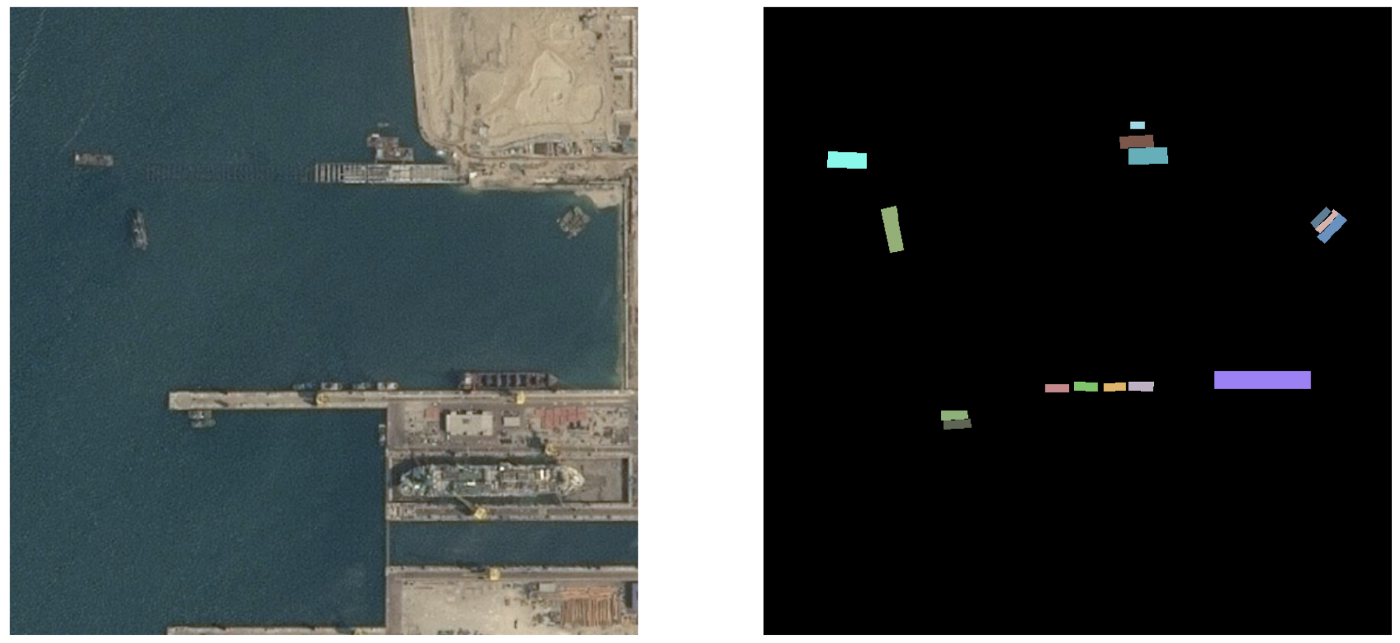
\includegraphics[width = 3.4in, height = 1.6in]{../images/class_imbalance.png}}
    \caption{Example class imbalance}
\end{figure}

\subsection{IOU}
The Jaccard Index or Intersection Over Union, also known as the Jaccard similarity coefficient, is a statistic (metric) used for gauging the similarity and diversity of sample sets. It was developed by Grove Karl Gilbert in 1884 as his ratio of verification (v),\textsuperscript{\cite{murphy1996finley}} and now is frequently referred to as the Critical Success Index in meteorology. It was later developed independently by Paul Jaccard, originally giving the French name coefficient de communauté.\textsuperscript{\cite{jaccard1912distribution}} The Jaccard coefficient measures similarity between finite sample sets, and is defined as the size of the intersection divided by the size of the union of the sample sets, here is the formula:

\begin{equation}
    J(A,B) = \frac{Area\; of\; Overlap}{Area\; of\; Union} = \frac{|A \cap B|}{|A \cup B|}
\end{equation}

Here is an example of using IOU on a stop sign, where the green bounding box is the ground truth (the right prediction) and the red bounding box is what the model predicted.

\vspace{0.1in}

\begin{figure}[H]
\centering
  \vspace{-0.1in}
    \centerline{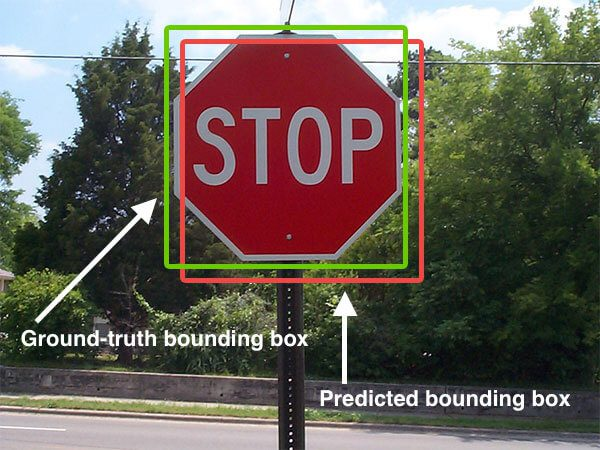
\includegraphics[width = 4in, height = 2.5in]{../images/exampleIOU.jpg}}
    \caption{Example of IOU applied on a stop sign image}
\end{figure}

\subsection{Dice}
The Sørensen–Dice coefficient is a statistic used to measure the similarity of two samples, It was developed by the botanists (scientific study of plants) Thorvald Sørensen and Lee Raymond Dice, who published in 1948 and 1945 respectively.\\
Sørensen's original formula was intended to be applied to discrete data. Given two sets, X and Y, it is defined as :
\begin{equation}
    DSC(X, Y) = \frac{2 | X \cap Y |}{| X |  +  | Y |}
\end{equation}
where |X| and |Y| are the cardinalities of the two sets . The Sørensen index equals twice the number of elements common to both sets divided by the sum of the number of elements in each set as we can see in fig \ref{fig:DSC_EX}. 
When applied to Boolean data, using the definition of true positive (TP), false positive (FP), and false negative (FN), it can be written as :
\begin{equation}
    DSC = \frac{2 TP}{2 TP + FN + FP}
\end{equation}

\begin{figure}[H]
\centering
  \vspace{-0.1in}
    \centerline{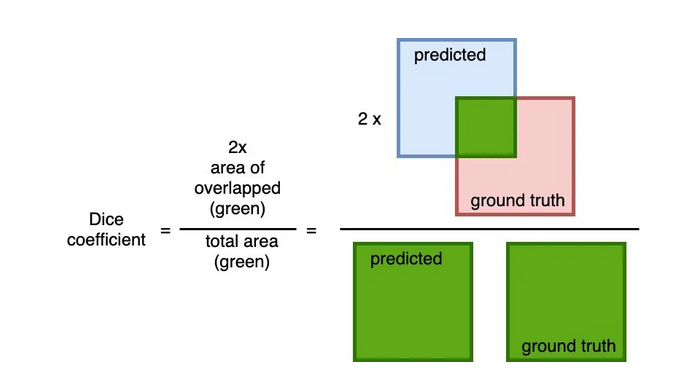
\includegraphics[width = 4in, height = 2.5in]{../images/DSC.png}}
    \caption{Example explaining Dice coefficient}
    \label{fig:DSC_EX}
\end{figure}


This coefficient is not very different in form from the Jaccard index (IOU). In fact, both are equivalent in the sense that given a value for the Sørensen–Dice coefficient $S$ , one can calculate the respective Jaccard index value $J$  and vice versa, using the equations : 
\begin{equation}
    J = \frac{DSC}{( 2 − DSC )}
\end{equation}

and 

\begin{equation}
    DSC = \frac{2 J  }{( 1 + J )}
\end{equation}

The function ranges between zero and one, like Jaccard. the corresponding loss function:
\begin{equation}
    DSC = 1 - \frac{2 TP}{2 TP + FN + FP}
\end{equation}

\subsection{Tversky}






\section{Conclusion}
\vspace{0.2in}
\hspace*{0.16in}

\newpage


\newpage

\vspace*{\fill}
\begin{center}
    {\color{Black} \rule{\linewidth}{1.2mm} }\\
\vspace{0.25in}
{\centering\fontsize{30}{40}{\bfseries{\color{Black}{\scshape{Chapter VI : Experiments And Results}}}}}
\vspace{0.35in}\\
    {\color{Black} \rule{\linewidth}{1.2mm} }
\end{center}
\vspace*{\fill}
\addcontentsline{toc}{chapter}{\color{Black}{Chapter VI : Experiments And Results}}
\setcounter{section}{0}

\newpage

\section{Introduction}
\vspace{0.2in}
\hspace{\parindent}
In this Section we will detail the different experiments and we will discuss the evaluation results obtained from the two segmentation models DO-UNet and DO-SegNet both with the BinaryCrossEnropy Loss Function. And we also discuss the evaluation results of the three counting algorithms Watershed, Circle Hough Transform and Connected Component Labeling for the three blood elements RBCs and WBCs and Platelets.

\section{Used Tools}
\subsection{TensorFlow}
\hspace{\parindent}
In our work we used TensorFlow which is an open source library developed by Google Brain Team for Artificial Intelligence, it contains multiple pre-defined models and algorithms for Deep Learning and Machine Learning, tensorFlow can be used in multiple languages as python, C++, Java and JavaScript.\\
Tensorflow can be used to Create, Train, Deploy Models. And when we talk about complicated models we can use Keras.
Keras is a high level API for Neural Networks which helps with experiments on the models and extensibility.

\begin{figure}[H]
    \centering
      \vspace{-0.1in}
        \centerline{
\includegraphics[width = 2.5in]{../images/tensorflow.png}}
        \caption{Tensorflow}
        \label{Tensorflow}
    \end{figure}

\subsection{Colab}
\hspace{\parindent}
Google Colab or Colaboratory is a free Jupyter notebook environment running on Google's cloud servers for machine learning training and research. This platform allows the user to leverage backend hardware such as GPUs and TPUs and train Machine Learning and Deep Learning models directly in the cloud. Without the need to install anything on our computer at the anything on our computer except a browser.
but it has some disadvantages where we have a limit on the GPU usage
and non presistant storage.

\begin{figure}[H]
\centering
  \vspace{-0.1in}
    \centerline{
\includegraphics[width = 2in]{../images/colab.png}}
    \caption{Google Colab}
    \label{Google Colab}
\end{figure}

\subsection{PaperSpace}
\hspace{\parindent}
Paperspace is a high-performance cloud computing and ML development platform for building, training and deploying machine learning models. It has a complete jupyter notebook environement which has a persistent storage and 6 hours limit for each execution.

\begin{figure}[H]
    \centering
      \vspace{-0.1in}
        \centerline{
\includegraphics[width = 3in]{../images/paperspace.png}}
        \caption{Paperspace}
        \label{Paperspace}
    \end{figure}

\section{do-U-Net Results}
\subsection{Red Blood Cells}
\hspace{\parindent}
The Red Blood Cells are the most difficult to detect because of the overlapping, where in some samples we can't notice the overlapping by eyes, in this experiment we are testing do-U-Net from \textsuperscript{\cite{10.1007/978-3-030-44584-3_31}}.
In the do-U-Net we updated the data augmentation phase. and applied Transfer Learning to get better edge mask. we can see in the dataset that we have only 13 images out of 108 from ALL-IDB1 that contains edge-masks and 108 masks, so the problem here is the lack of the edge label. we ended up with the method below as the best fit to our problem:

\begin{enumerate}
    \item Train the DO-Unet outputs on the big dataset (108 masks) which will output two identical masks.
    \item Continue Training the DO-Unet with the small dataset (13 masks, 13 edges), and Freeze the Mask Output.
\end{enumerate}

% 
% \usepackage{multirow}


\begin{table}[H]
\centering
\resizebox{\textwidth}{!}{\begin{tabular}{|c|l|c|c|c|c|c|c|c|} 
\hline
\textbf{RBC\_Model}  & \textbf{Dataset}                                                                                                                                & \textbf{Epochs}                                                                      & \textbf{Output}      & \textbf{Loss}        & \textbf{Mean IOU}    & \textbf{Dice}        & \textbf{Tversky}     & \textbf{Accuracy}     \\ 
\hline
\multirow{2}{*}{A}   & \multirow{2}{*}{\begin{tabular}[c]{@{}l@{}}small Dataset\\(mask + edge) * (10 + 3)\end{tabular}}                                                & \multirow{2}{*}{800}                                                                 & Mask                 & 0.3615               & 0.6365               & 0.8304               & 0.8232               & 0.8754                \\ 
\cline{4-9}
                     &                                                                                                                                                 &                                                                                      & Edge                 & 0.1816               & 0.0663               & 0.3582               & 0.3475               & 0.9343                \\ 
\hline
\multirow{2}{*}{B}   & \multirow{2}{*}{\begin{tabular}[c]{@{}l@{}}\makecell{Phase 1: big dataset mask*108\\Phase 2: small Dataset (mask + edge)*13}\end{tabular}} & \multirow{2}{*}{\begin{tabular}[c]{@{}l@{}}Phase 1: 120 \\Phase 2: 400\end{tabular}} & Mask                 & 0.0713               & 0.7751               & 0.9528               & 0.9567               & 0.9716                \\ 
\cline{4-9}
                     &                                                                                                                                                 &                                                                                      & Edge                 & 0.1465               & 0.0759               & 0.4127               & 0.4015               & 0.9385                \\ 
\hline
\multicolumn{1}{l}{} & \multicolumn{1}{l}{}                                                                                                                            & \multicolumn{1}{l}{}                                                                 & \multicolumn{1}{l}{} & \multicolumn{1}{l}{} & \multicolumn{1}{l}{} & \multicolumn{1}{l}{} & \multicolumn{1}{l}{} & \multicolumn{1}{l}{} 
\end{tabular}}
\label{table:do-unet-transfer}
\caption{Normal trained modes compared to transfer learning model}
\end{table}

The table \ref{table:do-unet-transfer} compares between the normal trained model A on the small dataset which contains 13 masks and edges and the model be which is trained on two phases, first with the big dataset (108 mask without edge) for 60 epochs, in the second phase we continued training with the small dataset (13 masks + edges) for 400 epochs.
We can see that this method pushed the edge accuracy which is really important to get rid of the overlapping.

After training the dual-output-U-Net model we did a benchmark on the 13 images to calculate the counting accuracy of the three methods, we ended up with the table \ref{table:DOUNET-RBC} below where we can see that the Circle hough transform method is the best for RBC counting with 95.36 accuracy, because all the RBCs have a similar shape and size.

\begin{table}[H]
\centering
\begin{tabular}{|  c | c | c | c | c | c | c | c |}
\hline
\textbf{Image} & \textbf{Real count} & \textbf{Watershed} & \textbf{CCL} & \textbf{CHT} & \textbf{Watershed\_acc} & \textbf{CCL\_acc} & \textbf{CHT\_acc} \\
\hline
Im037\_0 & 105 & 85 & 70 & 102 & 80.95 & 66.67 & 97.14 \\
Im045\_0 & 601 & 517 & 415 & 577 & 86.02 & 69.05 & 96.01 \\
Im053\_1 & 802 & 571 & 320 & 652 & 71.20 & 39.90 & 81.30 \\
Im001\_1 & 215 & 214 & 205 & 216 & 99.53 & 95.35 & 99.53 \\
Im004\_1 & 258 & 280 & 247 & 268 & 91.47 & 95.74 & 96.12 \\
Im015\_1 & 293 & 295 & 260 & 281 & 99.32 & 88.74 & 95.90 \\
Im022\_1 & 242 & 251 & 235 & 246 & 96.28 & 97.11 & 98.35 \\
Im050\_1 & 460 & 498 & 423 & 519 & 91.74 & 91.96 & 87.17 \\
Im069\_0 & 665 & 651 & 531 & 675 & 97.89 & 79.85 & 98.50 \\
Im079\_0 & 512 & 496 & 398 & 518 & 96.88 & 77.73 & 98.83 \\
Im095\_0 & 150 & 189 & 95 & 150 & 74.00 & 63.33 & 100.00 \\
Im099\_0 & 528 & 478 & 397 & 517 & 90.53 & 75.19 & 97.92 \\
Im108\_0 & 510 & 511 & 418 & 546 & 99.80 & 81.96 & 92.94 \\
\hline
\textbf{Total} &  &  &  &  & 90.43 & 78.66 & 95.36 \\
\hline
\end{tabular}
\caption{RBC Counting results using 3 algorithms}
\label{table:DOUNET-RBC}
\end{table}


\subsection{White Blood Cells}
\hspace{\parindent}
The White Blood Cells are also difficult to detect because of the non stable shape and in some cases they overlap, in this experiment we are comparing single output U-Net from \textsuperscript{\cite{10.1007/978-3-030-44584-3_31}} and the single output SegNet model.
In the UNet we removed the edge output because we don't have the edge annotation. then trained the model for 15 epochs with the binaryCrossEntropy Loss function on (74 + 34) images. 
We ended up with a very high accuracy and IOU score as we can see in table \ref{table:unet-wbc-training}.

\begin{table}[H]
\begin{tabular}{|l|l|l|l|l|l|l|}
\hline
\textbf{WBC Model} & \textbf{epochs} & \textbf{Loss}   &\textbf{Mean IOU} & \textbf{Dice}   & \textbf{Tversky} & \textbf{Accuracy} \\ \hline
UNet      & 15 & 0.0120 & 0.0162   & 0.0863 & 0.0863  & 0.9976   \\ \hline
\end{tabular}
\caption{WBC model performance}
\label{table:unet-wbc-training}
\end{table}

After training the model we did a benchmark on the 13 images then on the complete database (108 images) to calculate the counting accuracy of the three methods.\\ 
The real count of the 108 images is calculated manually because the original database dosn't have the count information. We ended up with the table \ref{table:UNet-WBC} below where we can see that the watershed method is the best for WBC counting with 97.94 accuracy on the 13 images and 95.64 on the complete database, because the white blood cells always slightly overlap each other where it's easy to the watershed to segment them.

\begin{table}[H]
\centering
\begin{tabular}{|  c | c | c | c | c | c | c | c |}
\hline
\textbf{Image} & \textbf{Real count} & \textbf{Watershed} & \textbf{CCL} & \textbf{CHT} & \textbf{Watershed\_acc} & \textbf{CCL\_acc} & \textbf{CHT\_acc} \\
\hline
Im037\_0 & 1 & 1 & 2 & 1 & 100.00 & 0.00 & 100.00 \\
Im045\_0 & 1 & 1 & 2 & 1 & 100.00 & 0.00 & 100.00 \\
Im053\_1 & 45 & 44 & 39 & 41 & 97.78 & 86.67 & 91.11 \\
Im001\_1 & 18 & 17 & 14 & 15 & 94.44 & 77.78 & 83.33 \\
Im004\_1 & 12 & 12 & 10 & 14 & 100.00 & 83.33 & 83.33 \\
Im015\_1 & 22 & 22 & 16 & 20 & 100.00 & 72.73 & 90.91 \\
Im022\_1 & 5 & 5 & 6 & 5 & 100.00 & 80.00 & 100.00 \\
Im050\_1 & 21 & 22 & 18 & 24 & 95.24 & 85.71 & 85.71 \\
Im069\_0 & 1 & 1 & 2 & 1 & 100.00 & 0.00 & 100.00 \\
Im079\_0 & 7 & 8 & 8 & 6 & 85.71 & 85.71 & 85.71 \\
Im095\_0 & 2 & 2 & 3 & 2 & 100.00 & 50.00 & 100.00 \\
Im099\_0 & 3 & 3 & 4 & 1 & 100.00 & 66.67 & 33.33 \\
Im108\_0 & 4 & 4 & 5 & 4 & 100.00 & 75.00 & 100.00 \\
\hline
\textbf{Total 13 images} &  &  &  &  & 97.94 & 58.74 & 88.7 \\
\textbf{Total 108 images} &  &  &  &  & 95.64 & 51.68 & 85.76 \\
\hline
\end{tabular}
\caption{WBC Counting results with 3 algorithms}
\label{table:UNet-WBC}
\end{table}

\subsection{platelets}
\hspace{\parindent}
The platelets are easy to count because of the rare overlapping but they are a bit difficult to segment because of their small size.\\
In this experiment we are testing single output U-Net from \textsuperscript{\cite{10.1007/978-3-030-44584-3_31}}. In the UNet we removed the edge output because we don’t have the edge annotation.
then trained the model for 50 epochs with the BinaryCrossEntropy Loss function on (74 + 34) images.
We ended up with a very high accuracy and IOU score as we can see in table \ref{table:PLT_DOUNET_TRAIN}.

\begin{table}
\centering
\begin{tabular}{|l|l|l|l|l|l|l|} 
\hline
\textbf{PLT\_Model} & \textbf{epochs} & \textbf{Loss}    & \textbf{Mean IOU} & \textbf{Dice}   & \textbf{Tversky} & \textbf{Accuracy}  \\ 
\hline
UNet       & 50 & 0.0156 & 0.1995   & 0.5085 & 0.5431  & 0.9946    \\
\hline
\end{tabular}
\caption{Platelets Model Performance}
\label{table:PLT_DOUNET_TRAIN}
\end{table}

After training the model we did a benchmark on the 13 images to calculate the counting accuracy of the three methods.
We are comparing to the real count wich is calculated by feeding the ground truth platelets masks to  the CCL algorithm. because the original database dosn't have the count information.\\
We ended up with the table \ref{table:PLT_UNET_RESULT} below where we can see that the CCL method is the best for WBC counting with 98.58 accuracy, because of the rare overlapping on each other where it’s easy to the CCL to segment them.

\begin{table}[H]
\centering
\begin{tabular}{|  c | c | c | c |}
\hline
\textbf{Image} & \textbf{Real count} & \textbf{CCL} & \textbf{CCL\_acc} \\
\hline
Im008\_1 & 6 & 6  & 100.0 \\
Im030\_1 & 12 & 12  & 100.0 \\
Im031\_1 & 26 & 27  & 96.15 \\
Im036\_0 & 34 & 35  & 97.05 \\
Im037\_0 & 6 & 6  & 100.0 \\
Im038\_0 & 31 & 30  & 96.77 \\
Im039\_0 & 39 & 40  & 97.43 \\
Im040\_0 & 53 & 50  & 94.33 \\
Im044\_0 & 36 & 36  & 100.0 \\
Im045\_0 & 39 & 39  & 100.0 \\
Im047\_0 & 33 & 32  & 96.96 \\
Im050\_1 & 9 & 9  & 100.0 \\
Im052\_1 & 4 & 4  & 100.0 \\
Im058\_1 & 11 & 11  & 100.0 \\
Im068\_0 & 9 & 9  & 100.0 \\
\hline
\textbf{Total} &  &  & 98.58\\
\hline
\end{tabular}
\caption{Platlets Counting results with Connected Component Labeling Algorithm}
\label{table:PLT_UNET_RESULT}
\end{table}

\section{SegNet Results}
\hspace{\parindent}
SegNet segmentation results were pretty accurate for white blood cells and platelets, as for red blood cells, the segmentation was done using dual output (mask and edge-mask) to get rid of overlapped cells.\\
Here are the results of the Mean Squared Error (MSE) loss function on each type of cell:

\begin{table}[H]
\centering
\resizebox{\textwidth}{!}{%
\begin{tabular}{|c|c|c|c|c|c|c|c|c|}
\hline
\textbf{SegNet}                           & \textbf{Output} & \textbf{Dataset}    & \textbf{Epochs}      & \textbf{Loss} & \textbf{Mean IOU} & \textbf{Dice} & \textbf{Tversky} & \textbf{Accuracy} \\ \hline
\multirow{2}{*}{\textbf{Red Blood Cells}} & \textbf{Mask}   & \multirow{2}{*}{13} & \multirow{2}{*}{700} & 0.0315        & 0.7660            & 0.8902        & 0.9072           & 0.9586            \\ \cline{2-2} \cline{5-9} 
                                          & \textbf{Edge}   &                     &                      & 0.0436        & 0.0664            & 0.3618        & 0.3637           & 0.9399            \\ \hline
\textbf{White Blood Cells}                & \textbf{Mask}   & 106                 & 80                   & 0.0021        & 0.0214            & 0.2512        & 0.2572           & 0.9972            \\ \hline
\textbf{Platelets}                        & \textbf{Mask}   & 102                 & 80                   & 0.0025        & 0.0001            & 0.0019        & 0.0031           & 0.9989            \\ \hline
\end{tabular}%
}
\caption{Result of SegNet segmentation}
\label{Result of SegNet segmentation}
\end{table}


\subsection{Red Blood Cells}
\hspace{\parindent}
For the dual-output SegNet model, the resulting segmented images were very good, sometimes better than the do-U-Net, though it is not as optimized when training and also predicting images, but it gets the job done with 95.86\% mask and 93.99\% edge accuracies. The segmented output images also had some noise which affected Connected Component Labeling (CCL) when counting.
As for Circle Hough Transform (CHT), the noise did not affect the result.
Red Blood Cells detection and counting is by far the hardest, because it is the only cell that overlaps and that makes it hard for counting.
The segmented output of do-SegNet is thresholded using a binary threshold, and then sent to 3 algorithms:

\begin{itemize}
  \item \textbf{Circle Hough Transform}: CHT was our best result for red blood cells counting, which achieved an accuracy of 94.03\% on the same dataset used for training the model (13 images with their respective masks and edge-masks).
  \item \textbf{Connected Component Labeling}: CCL was applied directly on the thresholded output edge, this method was far from accurate because the do-SegNet output had some noise (even when removing most of it), and also the overlapped nature of red blood cells which makes it very hard for this algorithm to count correctly. CCL achived an accuracy of 76.49\% counting red blood cells.
  \item \textbf{Euclidean Distance Transform}: EDT is used to get rid of the overlapped cells, also peak local max was applied on the EDT output for finding local maxima(s), the result of this approach is 84.64\% accuracy.
\end{itemize}

\begin{table}[H]
\centering
\begin{tabular}{|c|c|c|c|c|c|c|c|}
\hline
 \textbf{Image} & \textbf{Real\_Count} & \textbf{CHT} & \textbf{CCL} & \textbf{EDT} & \textbf{CHT\_acc} & \textbf{CCL\_acc} & \textbf{EDT\_acc} \\ \hline
 Im001\_1 & 215 & 212 & 234 & 247 & 98.6 & 91.16 & 85.12 \\ 
 Im004\_1 & 258 & 255 & 264 & 285 & 98.84 & 97.67 & 89.53 \\ 
 Im015\_1 & 293 & 269 & 212 & 261 & 91.81 & 72.35 & 89.08 \\ 
 Im022\_1 & 242 & 232 & 279 & 268 & 95.87 & 84.71 & 89.26 \\ 
 Im037\_0 & 105 & 103 & 75 & 88 & 98.1 & 71.43 & 83.81 \\ 
 Im045\_0 & 601 & 576 & 409 & 480 & 95.84 & 68.05 & 79.87 \\ 
 Im050\_1 & 460 & 486 & 450 & 475 & 94.35 & 97.83 & 96.74 \\ 
 Im053\_1 & 802 & 614 & 228 & 448 & 76.56 & 28.43 & 55.86 \\ 
 Im069\_0 & 665 & 653 & 376 & 549 & 98.2 & 56.54 & 82.56 \\ 
 Im079\_0 & 512 & 502 & 407 & 430 & 98.05 & 79.49 & 83.98 \\ 
 Im095\_0 & 150 & 177 & 177 & 170 & 82.0 & 82.0 & 86.67 \\ 
 Im099\_0 & 528 & 516 & 437 & 465 & 97.73 & 82.77 & 88.07 \\ 
 Im108\_0 & 510 & 528 & 418 & 458 & 96.47 & 81.96 & 89.8 \\ \hline
 Total & -1 & -1 & -1 & -1 & 94.03 & 76.49 & 84.64 \\ 

\hline
\end{tabular}
\caption{Results of each algorithm}
\label{Results of each algorithm}
\end{table}


\subsection{White Blood Cells}
\hspace{\parindent}
The results of white blood cells segmentation and counting using the SegNet model was very accurate achieving 99.72\% when segmenting.
White blood cells are the easiest out of the three, and the most accurate results.
However, white blood cells are different from the other cells because they come in different shapes and sizes, which made it hard to adapt each counting algorithm to every cell.\
The same counting methods are applied CHT, CCL and EDT. And each method had some drawbacks.\\
Here are the results:

\begin{itemize}
  \item \textbf{Circle Hough Transform}: Due to the different shapes of white blood cells, CHT achieved the lowest result which is 79.9\% counting accuracy, because some of the cells don't even look like circles and also their differet size which made it harder to count.
  \item \textbf{Connected Component Labeling}: CCL is similiar to CHT when it comes to white blood cells. And, because of the noisy outputs of SegNet the binary threshold can only do so much (it thresholdes some of the noise generated when predicting).\\
    CCl achieved an average counting accuracy of 82.89\%.
  \item \textbf{Euclidean Distance Transform}: EDT is the contender of white blood cells counting, because the distance transform gets rid of the noise completely and peak local max was very helpfull in eliminating that noise and getting an accurate count.\\
    This method achived a counting accuracy of 96.43\%.
\end{itemize}

Here are the results of the 13 images:

\begin{table}[H]
    \centering
    \begin{tabular}{|c|c|c|c|c|c|c|c|}
    \hline
     \textbf{Image} & \textbf{Real\_Count} & \textbf{CHT} & \textbf{CCL} & \textbf{EDT} & \textbf{CHT\_acc} & \textbf{CCL\_acc} & \textbf{EDT\_acc} \\ \hline
     Im001\_1 & 18 & 13 & 13 & 16 & 72.22 & 72.22 & 88.89 \\ 
     Im004\_1 & 12 & 11 & 9 & 12 & 91.67 & 75.0 & 100.0 \\ 
     Im015\_1 & 22 & 18 & 15 & 21 & 81.82 & 68.18 & 95.45 \\ 
     Im022\_1 & 5 & 5 & 5 & 5 & 100.0 & 100.0 & 100.0 \\ 
     Im037\_0 & 1 & 0 & 1 & 1 & 0 & 100.0 & 100.0 \\ 
     Im045\_0 & 1 & 1 & 1 & 1 & 100.0 & 100.0 & 100.0 \\ 
     Im050\_1 & 21 & 29 & 20 & 21 & 61.9 & 95.24 & 100.0 \\ 
     Im053\_1 & 45 & 44 & 43 & 44 & 97.78 & 95.56 & 97.78 \\ 
     Im069\_0 & 1 & 1 & 1 & 1 & 100.0 & 100.0 & 100.0 \\ 
     Im079\_0 & 7 & 7 & 9 & 9 & 100.0 & 71.43 & 71.43 \\ 
     Im095\_0 & 2 & 2 & 2 & 2 & 100.0 & 100.0 & 100.0 \\ 
     Im099\_0 & 3 & 1 & 3 & 3 & 33.33 & 100.0 & 100.0 \\ 
     Im108\_0 & 4 & 4 & 8 & 4 & 100.0 & 0 & 100.0 \\ \hline
     Total & -1 & -1 & -1 & -1 & 79.9 & 82.89 & 96.43 \\ 
    
    \hline
    \end{tabular}
    \caption{Results of wbc segnet}
    \label{Results of wbc segnet}
    \end{table}
    

\subsection{Platelets}
\hspace{\parindent}
The platelets segmentation result we achieved is not the best compared to the do-U-Net model. Segnet extracts the platelets but with some noise which made it very hard to count accurately.
It achieved a segmetation accuracy of 99.89\% and the highest counting accuracy is 71.56\% which is not very good.\\
Here are all the counting accuracies for each approach:

\begin{table}[H]
\centering
\begin{tabular}{|c|c|c|c|c|c|c|c|}
\hline
 \textbf{Image} & \textbf{Real\_Count} & \textbf{CHT} & \textbf{CCL} & \textbf{EDT} & \textbf{CHT\_acc} & \textbf{CCL\_acc} & \textbf{EDT\_acc} \\ \hline
 Im001\_1 & 0 & 0 & 0 & 0 & 100.0 & 100.0 & 100.0 \\ 
 Im004\_1 & 4 & 2 & 3 & 2 & 50.0 & 75.0 & 50.0 \\ 
 Im015\_1 & 7 & 1 & 2 & 1 & 14.29 & 28.57 & 14.29 \\ 
 Im022\_1 & 15 & 8 & 10 & 8 & 53.33 & 66.67 & 53.33 \\ 
 Im037\_0 & 6 & 5 & 6 & 5 & 83.33 & 100.0 & 83.33 \\ 
 Im045\_0 & 39 & 24 & 25 & 24 & 61.54 & 64.1 & 61.54 \\ 
 Im050\_1 & 10 & 8 & 8 & 8 & 80.0 & 80.0 & 80.0 \\ 
 Im053\_1 & 12 & 9 & 12 & 9 & 75.0 & 100.0 & 75.0 \\ 
 Im069\_0 & 3 & 3 & 3 & 3 & 100.0 & 100.0 & 100.0 \\ 
 Im079\_0 & 0 & 2 & 3 & 2 & 0.0 & 0.0 & 0.0 \\ 
 Im095\_0 & 7 & 6 & 6 & 6 & 85.71 & 85.71 & 85.71 \\ 
 Im099\_0 & 37 & 26 & 26 & 26 & 70.27 & 70.27 & 70.27 \\ 
 Im108\_0 & 5 & 6 & 7 & 6 & 80.0 & 60.0 & 80.0 \\ \hline
 Total &   &   &   &   & 65.65 & 71.56 & 65.65 \\ 

\hline
\end{tabular}
\caption{Platelets counting results using 3 algorithms}
\label{Platelets counting results using 3 algorithms}
\end{table}


\section{Results}
\vspace{0.2in}
\hspace{\parindent}

\begin{figure}[H]
\centering
\begin{minipage}{.5\textwidth}
  \centering
  \fbox{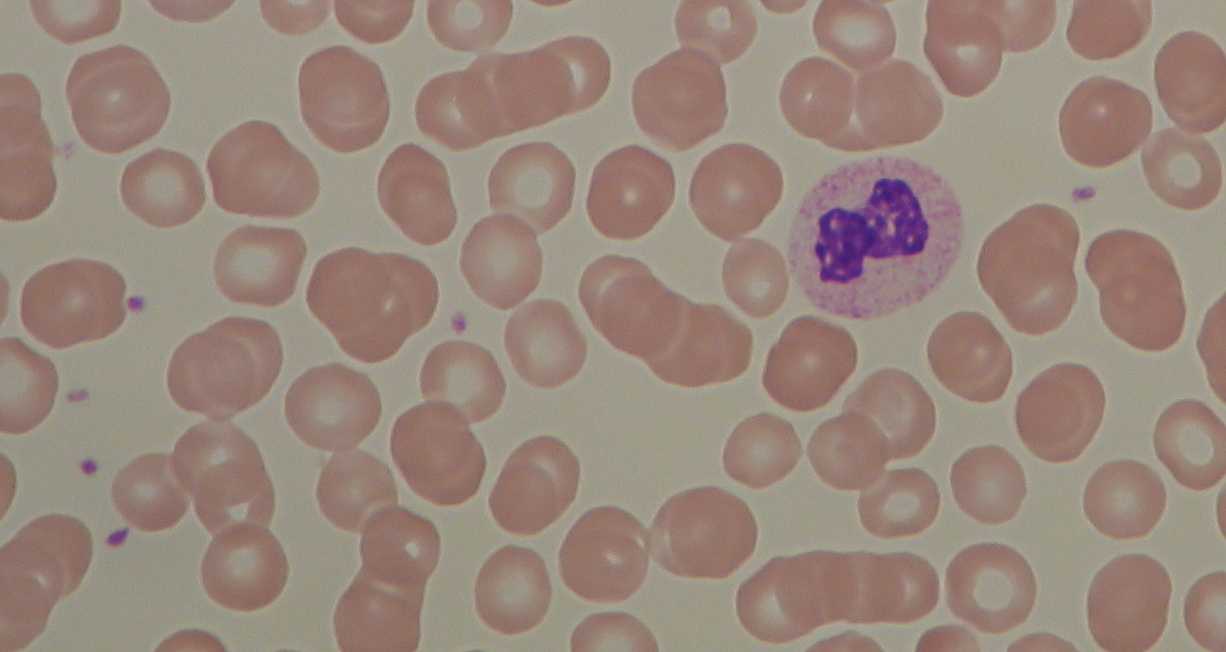
\includegraphics[width = 2.8in]{../images/originalCHT.jpg}}
  \subcaption{Original image}
\end{minipage}%
\begin{minipage}{.5\textwidth}
  \centering
  \fbox{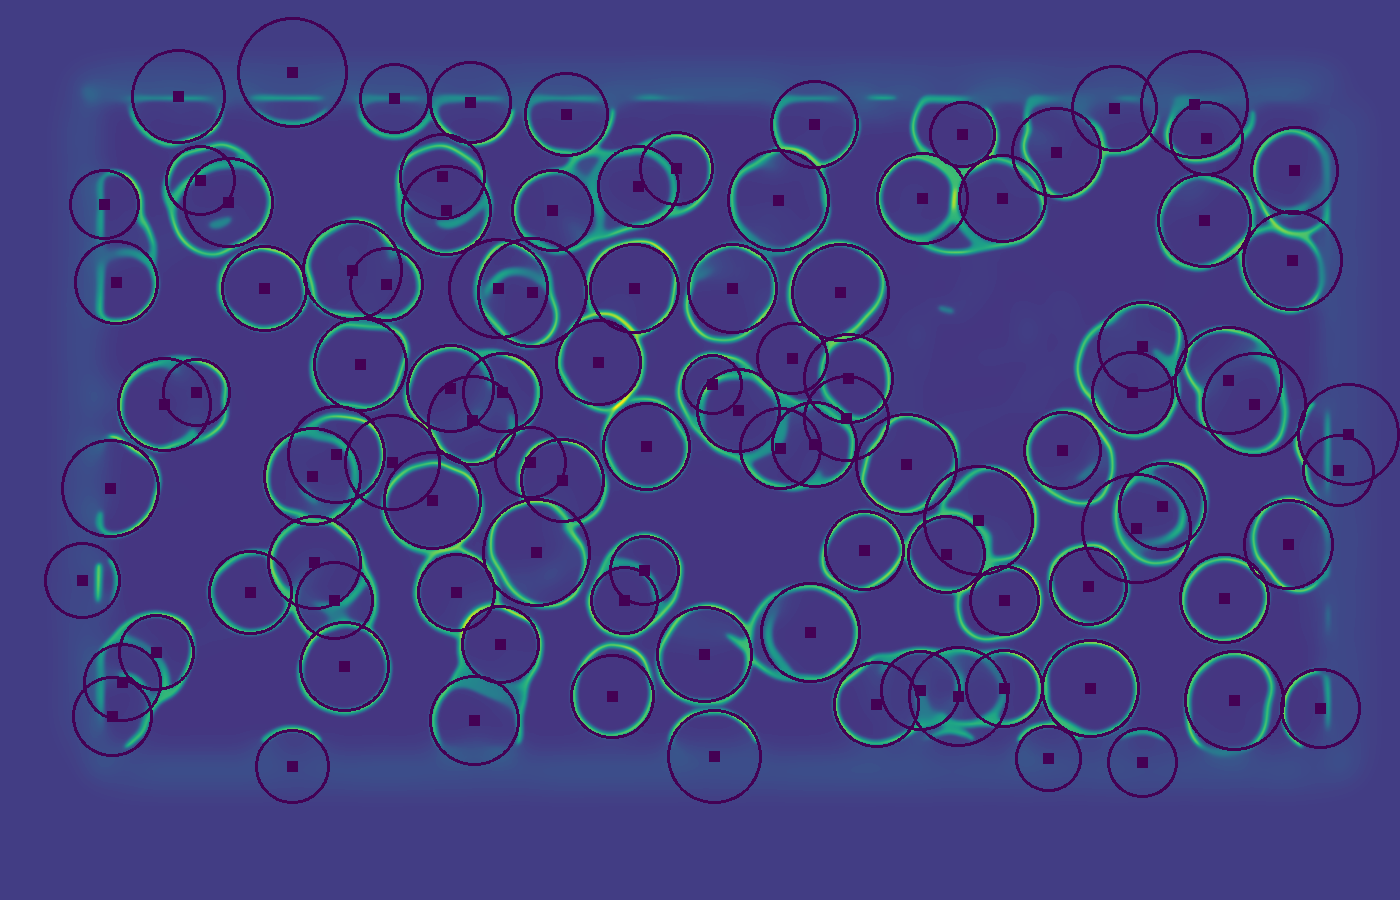
\includegraphics[width = 3.2in]{../images/cht.png}}
  \subcaption{Output CHT image}
\end{minipage}
  \caption{Circle Hough Transform applied to count red blood cells}
\end{figure}

\begin{figure}[H]
\centering
\begin{minipage}{.5\textwidth}
  \centering
  \fbox{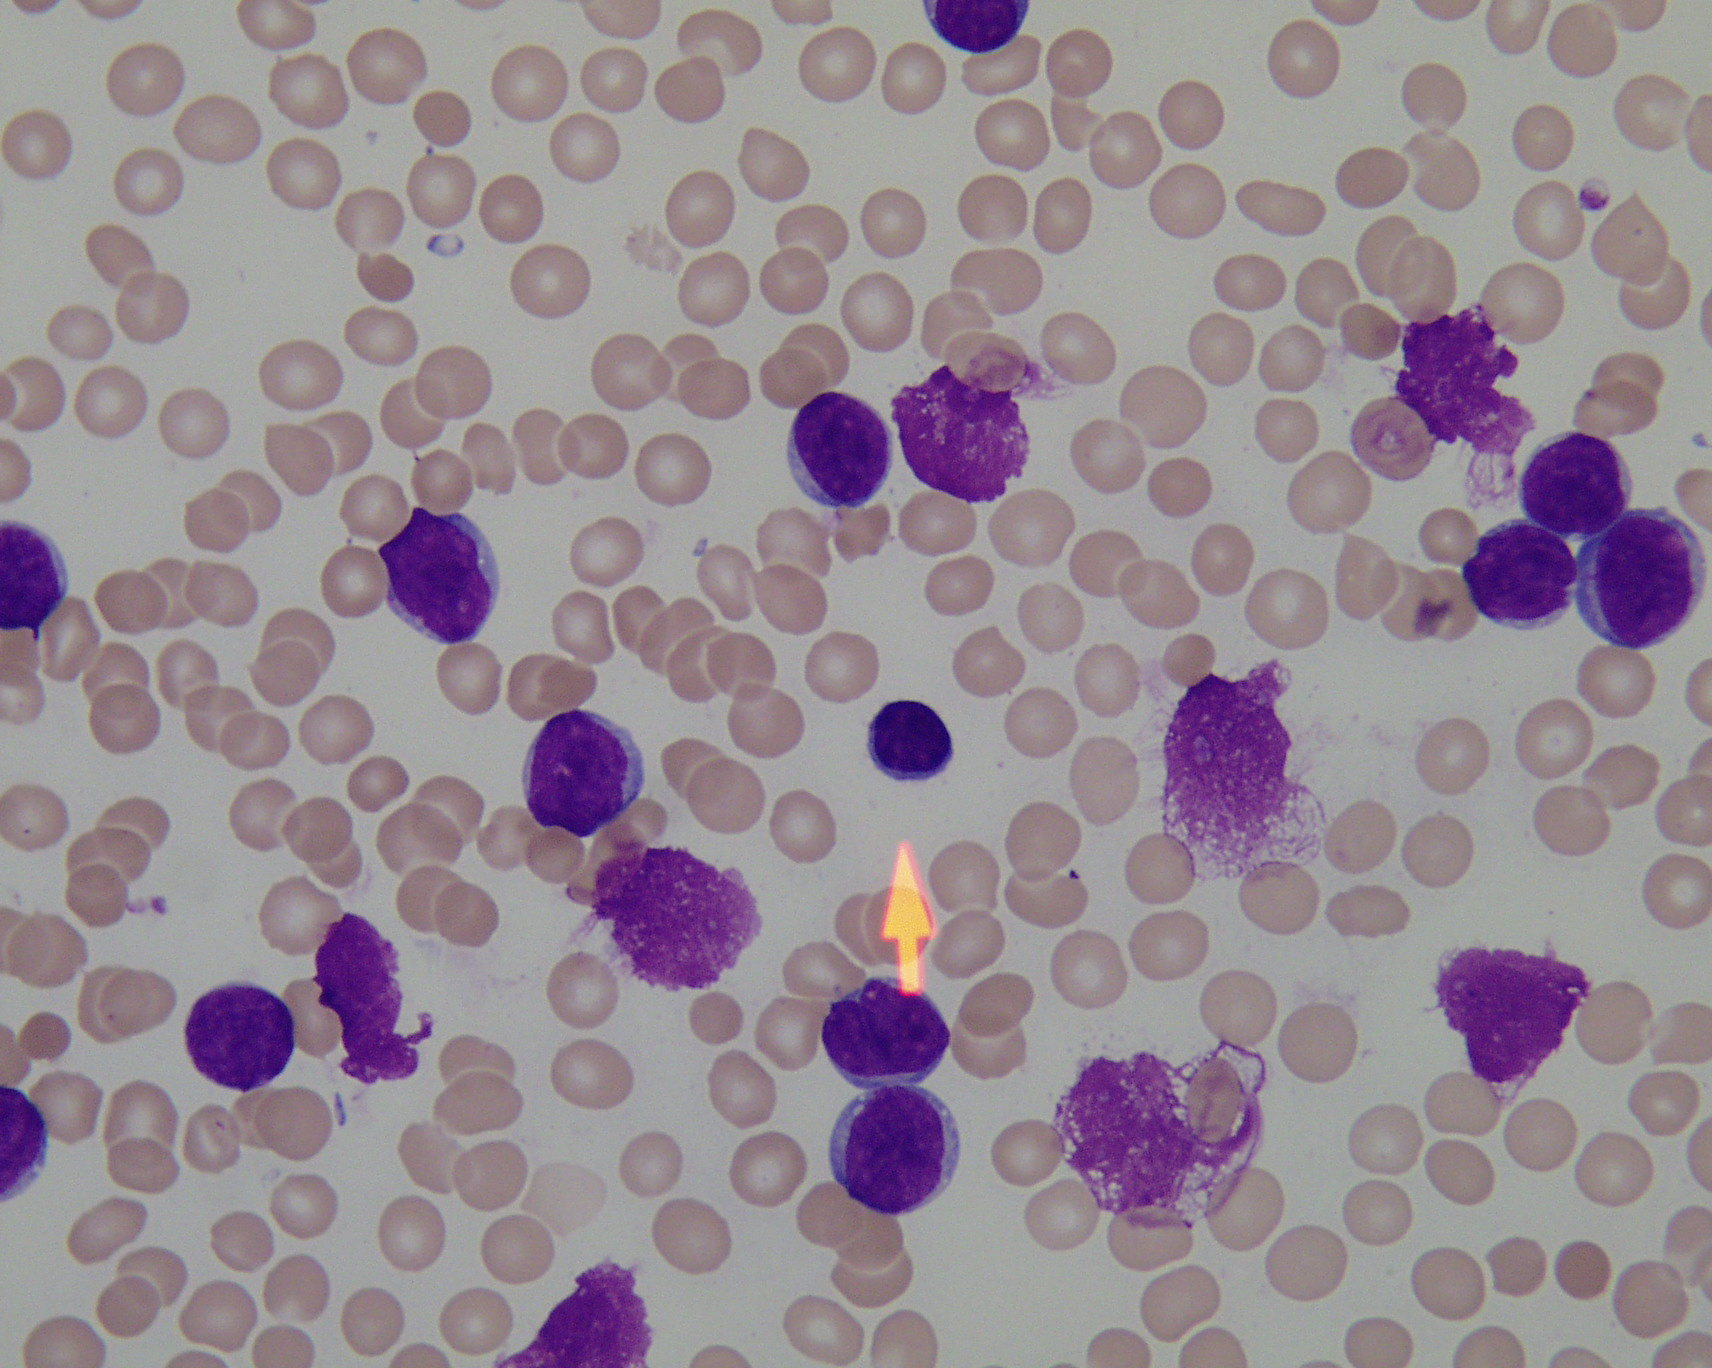
\includegraphics[width = 2.8in]{../images/originalWatershed.jpg}}
  \subcaption{Original image}
\end{minipage}%
\begin{minipage}{.5\textwidth}
  \centering
  \fbox{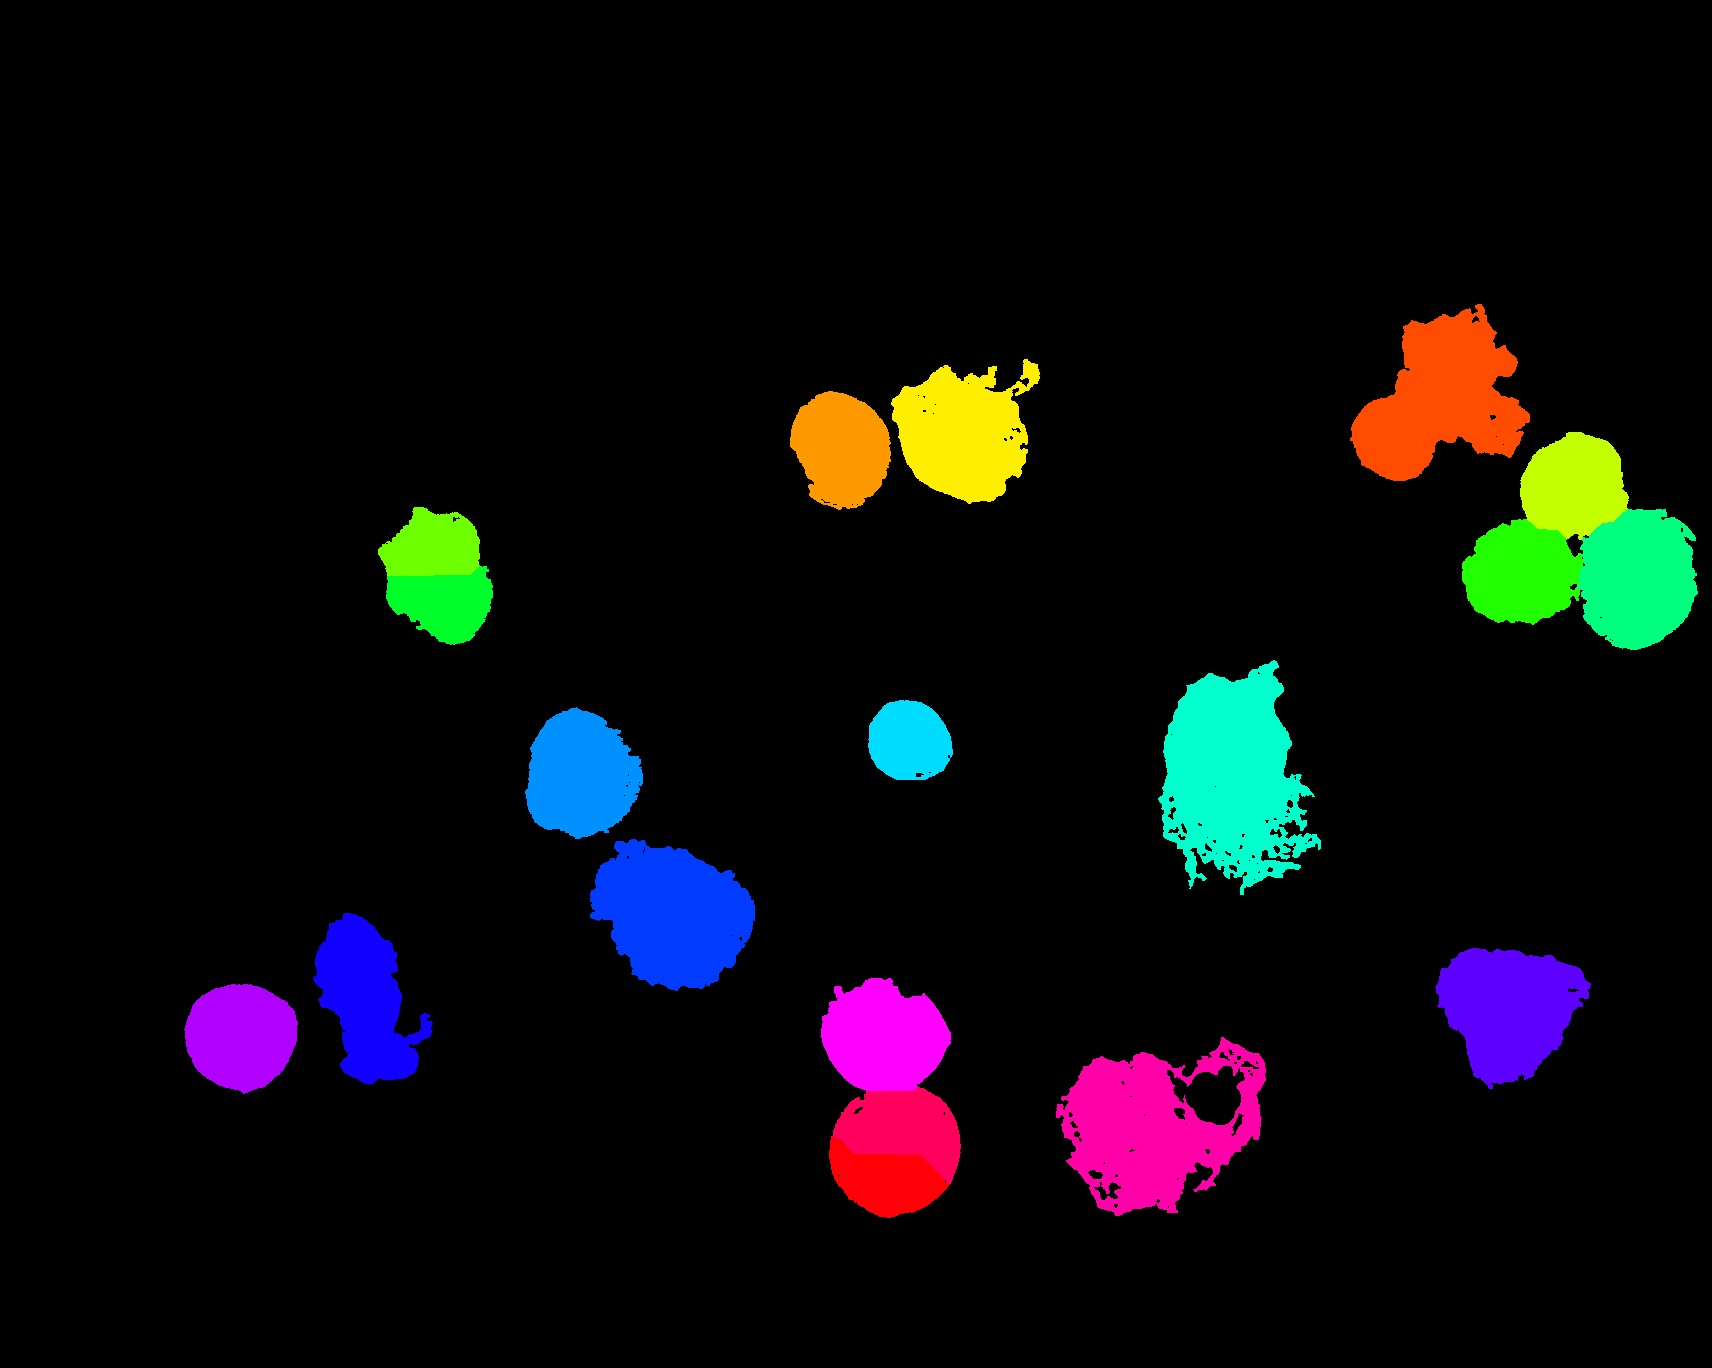
\includegraphics[width = 2.8in]{../images/watershed_color.jpg}}
  \subcaption{Output Watershed image}
\end{minipage}
  \caption{Watershed applied to count white blood cells}
\end{figure}

\begin{figure}[H]
\centering
\begin{minipage}{.5\textwidth}
  \centering
  \fbox{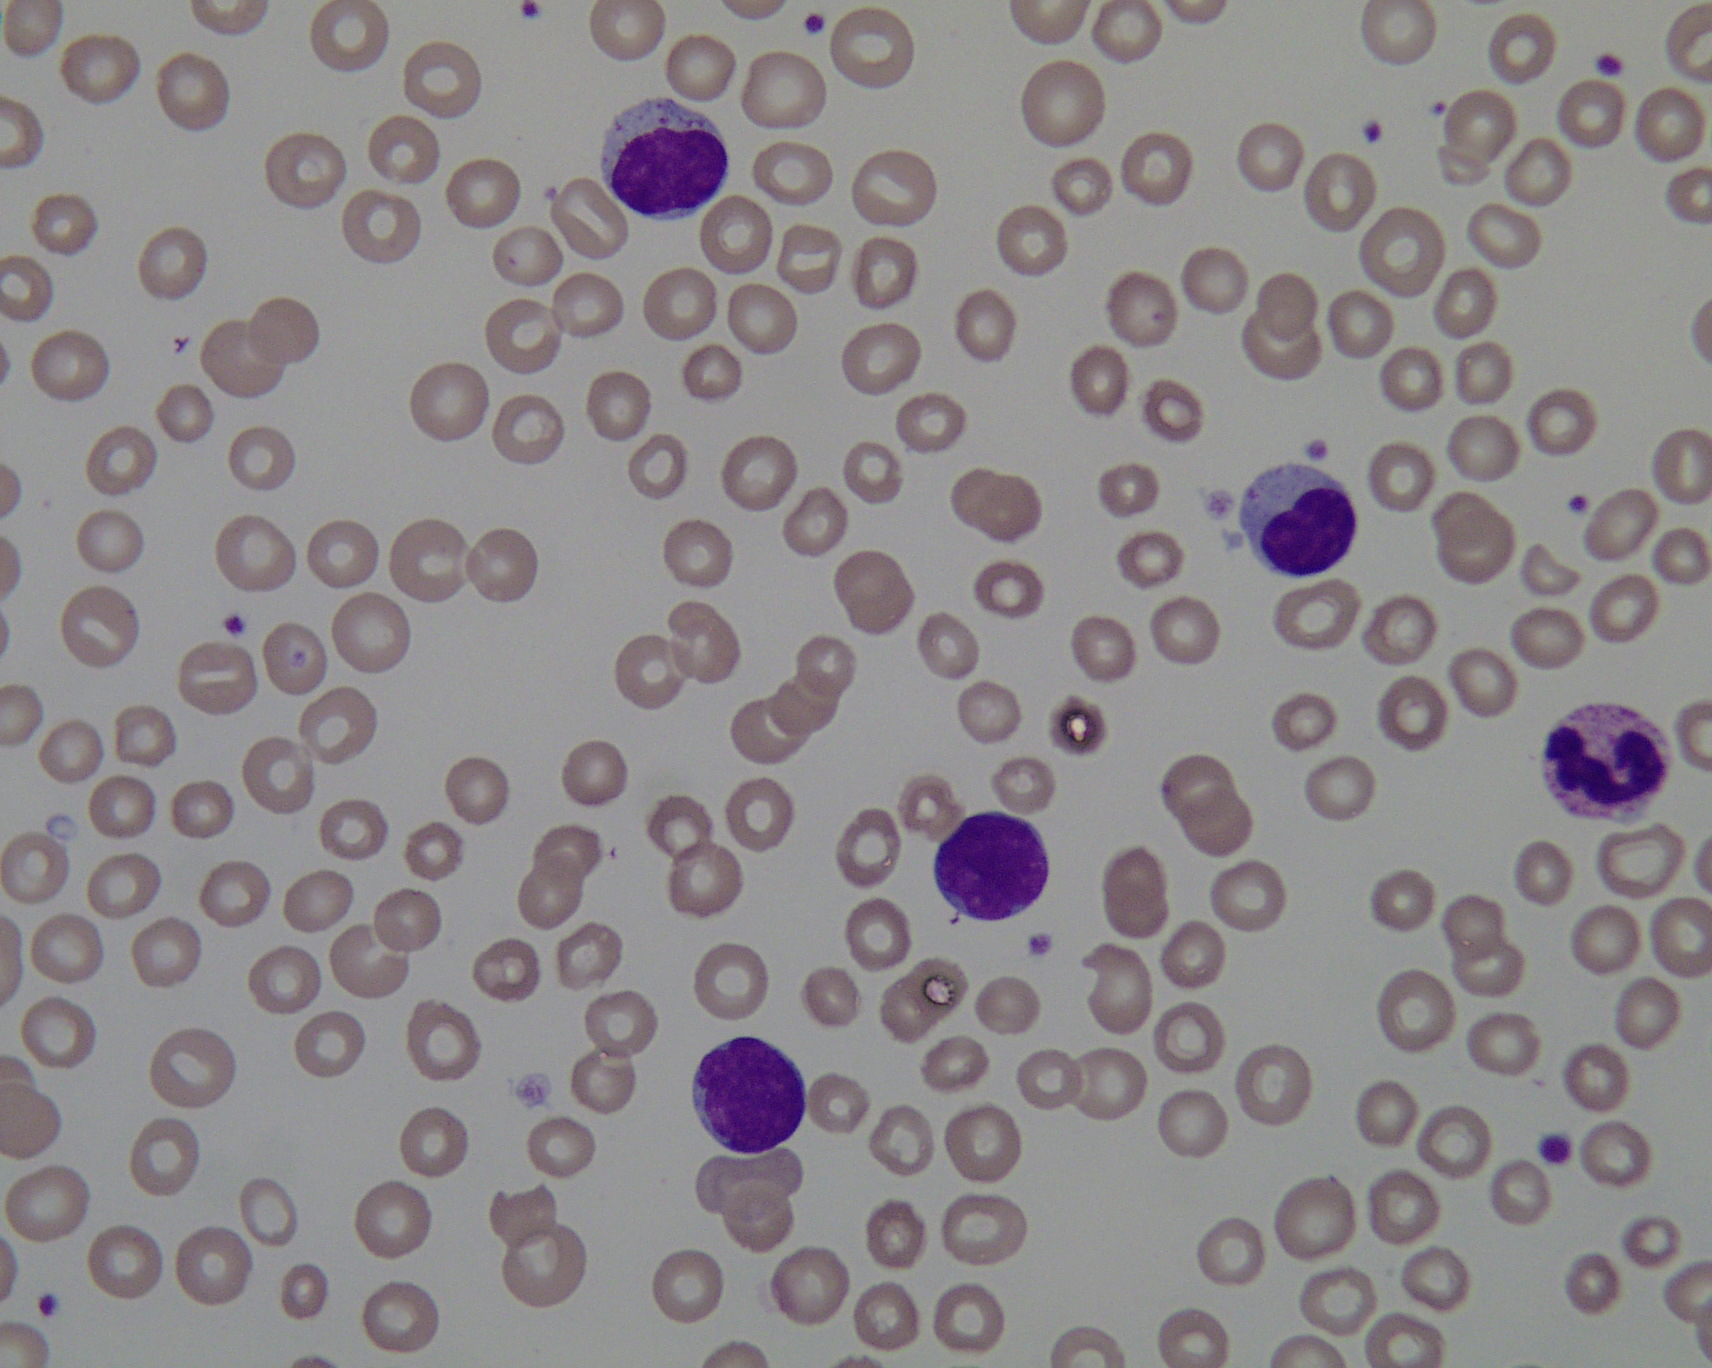
\includegraphics[width = 2.8in]{../images/originalCCL.jpg}}
  \subcaption{Original image}
\end{minipage}%
\begin{minipage}{.5\textwidth}
  \centering
  \fbox{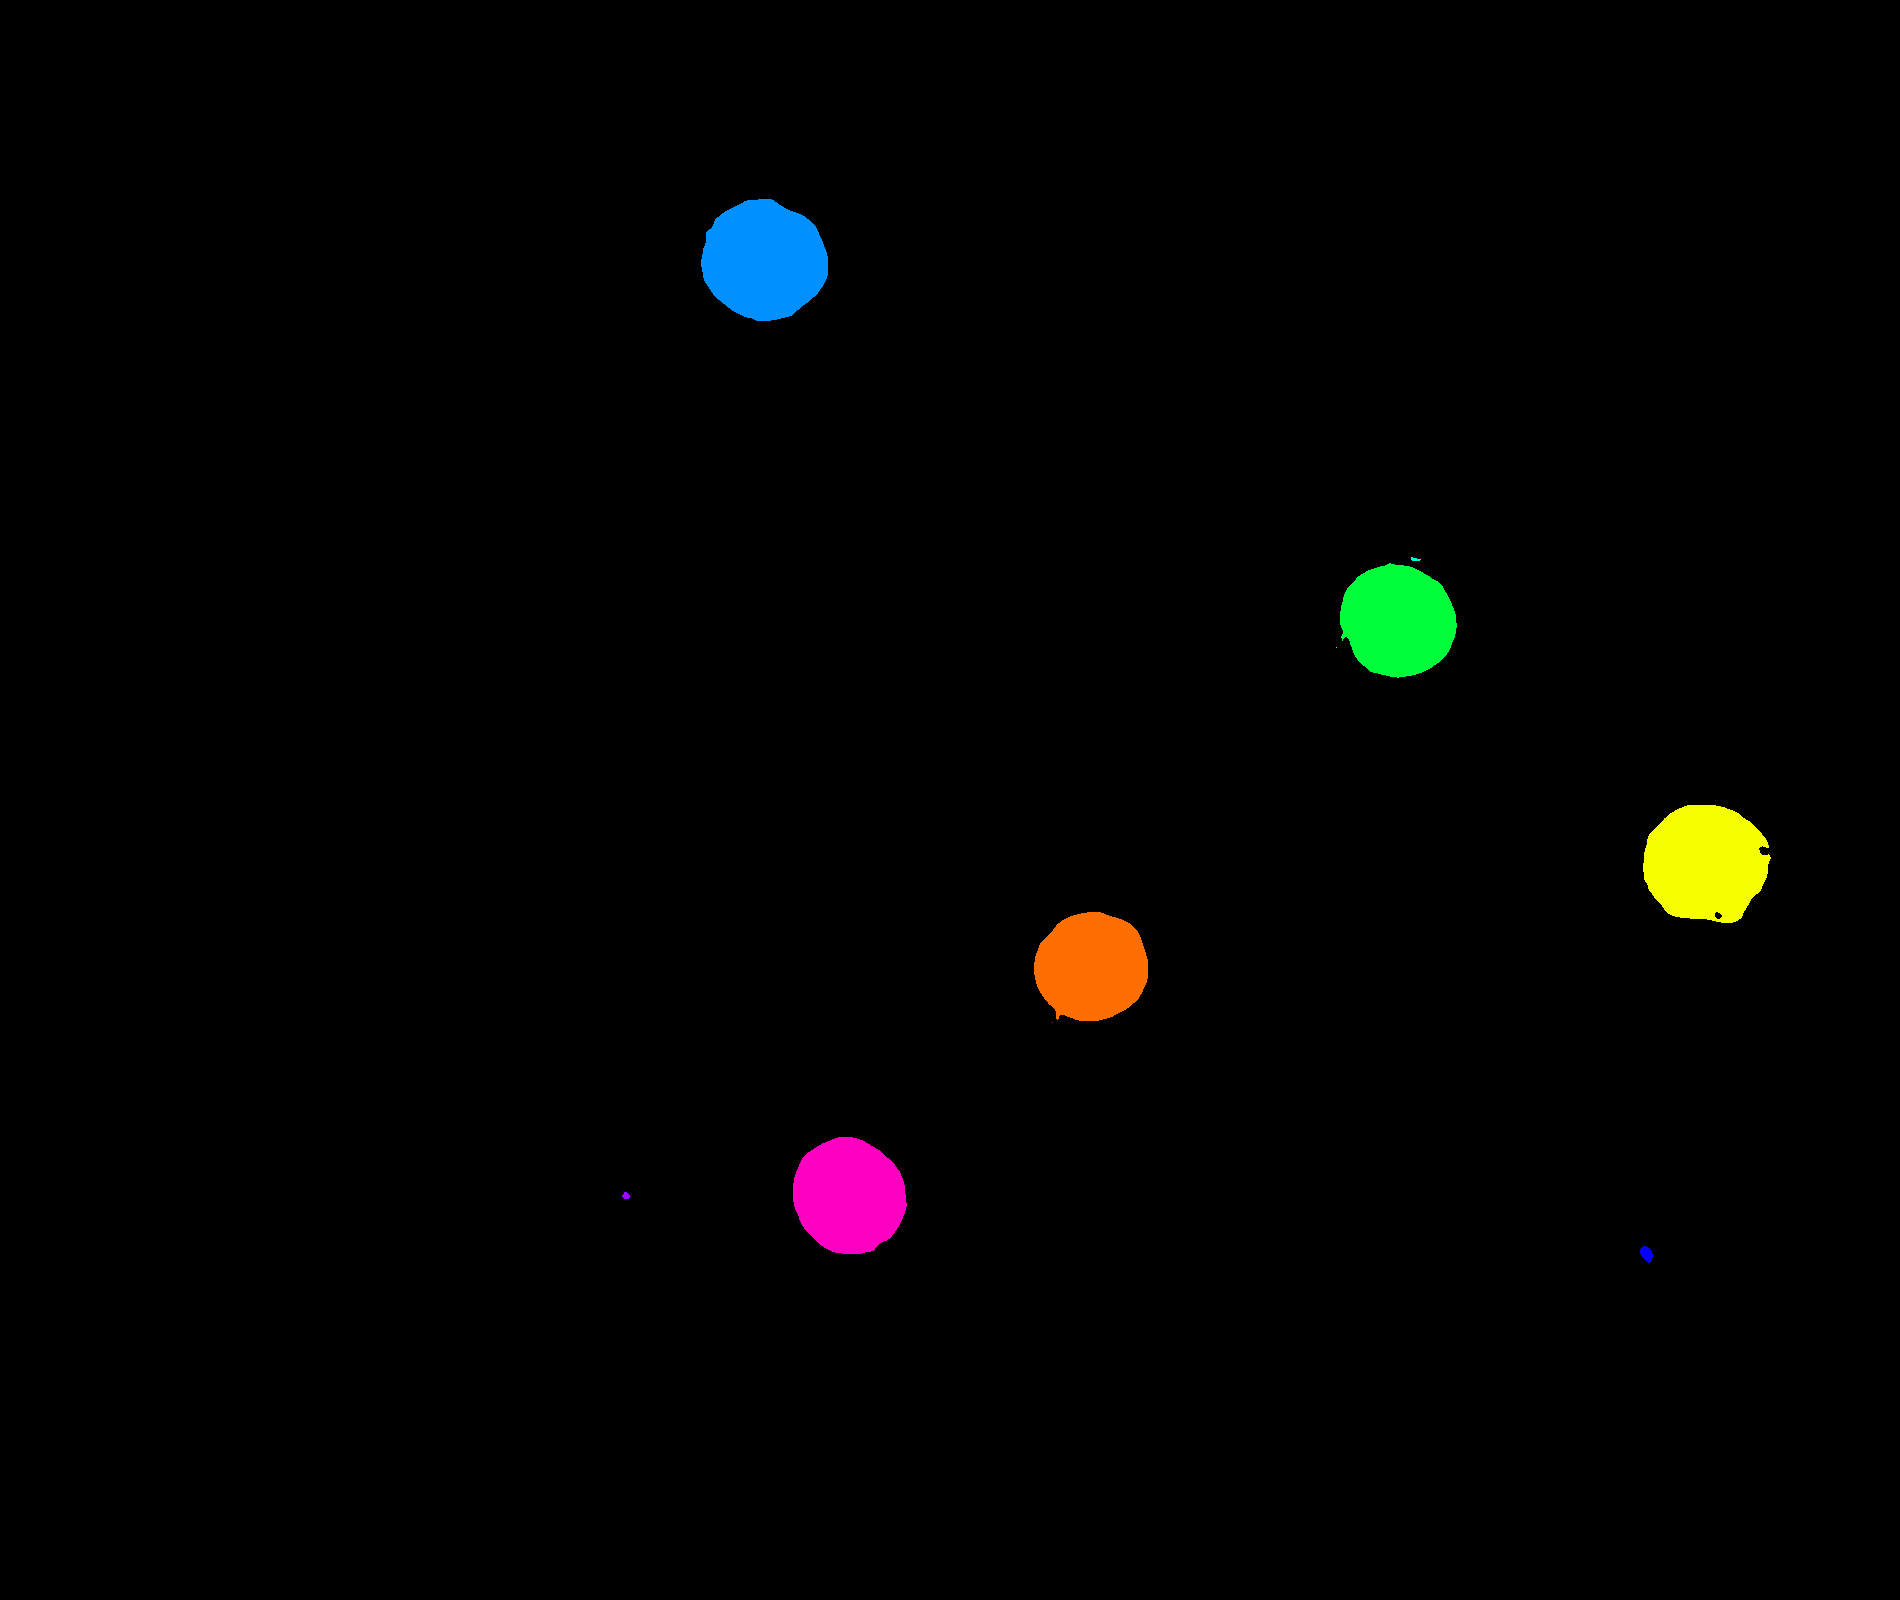
\includegraphics[width = 2.8in]{../images/ccl.png}}
  \subcaption{Output CCL image}
\end{minipage}
  \caption{Connected Component Labeling applied to count white blood cells}
\end{figure}

\section{Conclusion}
In conclusion, both models performed very well detecting and counting the blood cells, each one with its advantages and disadvateges.
But the do-UNet model outperformed SegNet because of the noise generating using segnet.

\newpage


\newpage

\vspace*{0.2in}

\begin{center}
    {\color{Black} \rule{4in}{1.4mm} }\\
    \vspace{0.1in}
    \scshape{\fontsize{34}{46}{\bfseries{\color{Black}{Conclusion}}}}
    \\
    \vspace{0.6in}
\end{center}
\cftaddtitleline{toc}{part}{\vspace{-0.12in}\color{Black}{Conclusion}}{}
\begin{changemargin}{0.9cm}{0.9cm}
\hspace*{0.16in}
\end{changemargin}

In the present work, we have mainly presented two different models of segmentation based on CNNs and three counting algorithms to perform a complete blood count.
We focused more on the segmentation task where  we tested two models U-Net and SegNet to get better masks. 

We can see that the U-Net gave better result with less noisy mask, but the two models has some weaknesses with the images color space, because both models takes rgb images therefore they depend a lot on the color features, for example if we slightly change the colors of the input image we get a big diffrence in the output mask.
In the counting task, we had a small time window where we couldn't tune the 3 three algorithm parameters to get the best results. but we got acceptable results in each blood cell type, especially with platelets.\\

As a future work, we can combine between the two models to benefit the strength points of both models, we can also find more combinations between edge and mask.\\
For the counting we can assign a weight for each  method to get a mean value from the 3 methods. And it would be interesting to develop a system which makes it possible to classify each blood cell depending on the shape and size and color to detect even more sophisticated abnormalities more accurate than the complete blood count.


\newpage

\bibliography{main}

\end{document}
